%%%%%%%%%%%%%%%%%%%%%%%%%%%%%%%%%%%%%%%%%%%%%%%%%%%%%%%%%%%%%%%%%%%%%%%
% Universidade Federal de Santa Catarina             
% Biblioteca Universitária                     
%                                                           
% (c)2010 Roberto Simoni (roberto.emc@gmail.com)
%         Carlos R Rocha (cticarlo@gmail.com)
%%%%%%%%%%%%%%%%%%%%%%%%%%%%%%%%%%%%%%%%%%%%%%%%%%%%%%%%%%%%%%%%%%%%%%%
\documentclass{ufscThesis}

%%%%%%%%%%%%%%%%%%%%%%%%%%%%%%%%%%%%%%%%%%%%%%%%%%%%%%%%%%%%%%%%%%%%%%%
% Pacotes usados especificamente para este documento
% Definidos pelo criador do documento
%%%%%%%%%%%%%%%%%%%%%%%%%%%%%%%%%%%%%%%%%%%%%%%%%%%%%%%%%%%%%%%%%%%%%%%
\usepackage{graphicx}
\usepackage{lscape}
\usepackage{multirow}
\usepackage{tabularx,calc}

%\renewcommand{\theequation}{\arabic{equation}} %se desejar tirar o capitulo

%\usepackage[labelsep=period]{caption} % O separador de legenda é um .
\usepackage[labelsep=endash]{caption} % O separador de legenda é um -

%%%%%%%%%%%%%%%%%%%%%%%%%%%%%%%%%%%%%%%%%%%%%%%%%%%%%%%%%%%%%%%%%%%%%%%
% Identificadores do trabalho
% Usados para preencher os elementos pré-textuais
%%%%%%%%%%%%%%%%%%%%%%%%%%%%%%%%%%%%%%%%%%%%%%%%%%%%%%%%%%%%%%%%%%%%%%%
\instituicao[a]{Universidade Federal de Santa Catarina} % Opcional
\departamento[a]{Programa de Pós-graduação em Ciência da Computação}
\curso[a]{Universidade Federal de Santa Catarina}
\documento[a]{Dissertação} % Opcional (Tese é o padrão)
\titulo{Modelagem de Aspectos por Múltiplos Pontos de Vista}
\autor{Pedro Ghilardi}
\data{14}{junho}{2013}   
\orientador[Orientador]{Ricardo Pereira e Silva, Prof. Dr.}
\coordenador[Coordenador]{Ronaldo dos Santos Mello, Prof. Dr.}                        

\numerodemembrosnabanca{5} % Isso decide se haverá uma folha adicional
%\orientadornabanca{sim} % Se faz parte da banca definir como sim
\bancaMembroA{Antônio Augusto Fröhlich, Prof. Dr.} %Nome do presidente da banca
\bancaMembroB{Marcello Thiry, Prof. Dr.} % Nome do membro da Banca
\bancaMembroC{Patrícia Vilain, Prof. Dr.} % Nome do membro da Banca

%%% Sobre a Banca
\dedicatoria{A minha família.}

\agradecimento{Ao meu orientador, Ricardo, pela sua orientação, compreensão e motivação. A minha namorada, Kaila, pela compreensão e auxílio nos
momentos que mais necessitei e a minha família que mesmo longe sempre me apoiou.}

\epigrafe{}{}

\textoResumo{A modelagem de sistemas orientados a aspectos tem como objetivo aumentar o nível de abstração de código para modelos. Esta dissertação
propõe a modelagem de sistemas orientados a aspectos usando UML, através de um perfil UML, abrangendo as características da programação orientada a
aspectos, e possibilitando a alternância de visões da dinâmica do sistema. O desenvolvedor pode criar diferentes composições de interesses núcleo e 
entrecortantes, visualizando os interesses núcleo, entrecortantes, ou uma composição com os interesses núcleos junto com os interesses entrecortantes. 
A visualização da dinâmica de aspectos pode ser atualizada dinamicamente, atualizando o modelo composto, sem esforço do desenvolvedor. Os interesses
são diferenciados no modelo composto através de diferentes cores. A solução proposta é implementada como uma ferramenta no ambiente SEA, 
a qual permite a geração automática de diagramas de sequência, resultantes da composição de aspectos. A abordagem de modelagem 
foi aplicada em um sistema de gerenciamento de hotel. Com a modelagem deste exemplo
conclui-se que a proposta permite representar de forma completa um sistema orientado a aspectos, como a especificação de wildcards, pontos de corte complexos
e todos os tipos de avisos da linguagem AspectJ. Realiza-se também uma comparação da abordagem proposta com outras abordagens da literatura. Nesta
comparação, a abordagem proposta destaca-se por permitir a alternância de visões e uma modelagem completa de aspectos.}
\palavrasChave {Modelagem Meta-Modelagem UML Aspectos Programação Orientada a Aspectos Interesses Perfil}

\textAbstract {The modeling of aspect-oriented systems has as one of its objectives to grow the abstraction level from code to models. This work
proposes an aspect-oriented modeling approach using the UML, through a UML profile, covering the features of the aspect-oriented programming,
enabling the intertwining of views of the system dynamics. The modeler may create different compositions of the core and crosscutting concerns,
viewing only the core concerns, the crosscutting ones, or a composition of both. The visualization of the aspect dynamic may be updated without
effort, updating the compound model. The concerns are differentiated in the compound model through different colors. The proposed solution is
implemented as a tool in the SEA environment, which allows the automatic generation of sequence diagramas, resulting from the aspect composition. The
modeling approach was applied in a hotel management system. This modeling example shows that the proposal allows to represent all the characteristics
of aspects, as the specification of wildcards, complex pointcuts and all the AspectJ advice types. In the related work comparison, this approach
highlights because it allows to enable the alternating of views and a full modeling of aspects.}
\keywords {Modeling Meta-Modeling UML Aspects Aspect-Oriented Programming Concerns Profile}


%%%%%%%%%%%%%%%%%%%%%%%%%%%%%%%%%%%%%%%%%%%%%%%%%%%%%%%%%%%%%%%%%%%%%%%
% Início do documento                                
%%%%%%%%%%%%%%%%%%%%%%%%%%%%%%%%%%%%%%%%%%%%%%%%%%%%%%%%%%%%%%%%%%%%%%%
\begin{document}

%--------------------------------------------------------
% Elementos pré-textuais
\capa  
\folhaderosto[comficha] 
\folhaaprovacao
\paginadedicatoria
\paginaagradecimento
\paginaresumo
\paginaabstract
\listadefiguras
\listadetabelas 
\listadeabreviaturas
\sumario

%-------------------------------------------------------------------------------
% Para listagens de algoritmos e de código, recomenda-se consultar os
% pacotes algorithms e lstlistings, que são usados para definir esses
% dois tipos de elementos de texto e possuem os comandos
% \listofalgorithms e \lstlistoflistings, respectivamente.
%-------------------------------------------------------------------------------

%--------------------------------------------------------
% Elementos textuaisf

\chapter{Introdu��o}

Este cap�tulo contextualiza o tema deste trabalho, apresentando motiva��es para o uso da programa��o orientada a aspectos e a necessidade de realizar
a modelagem de sistemas orientados a aspectos. Apresentam-se os objetivos, a metodologia da pesquisa e a justificativa para realiza��o do estudo. Ao
final, apresentam-se os resultados esperados, as limita��es e a organiza��o desta disserta��o.

\section{Contextualiza��o}

A Programa��o Orientada a Objetos (POO) \sigla{POO}{Programa��o Orientada a Objetos} � um paradigma de programa��o amplamente difundido e utilizado
para o desenvolvimento de aplica��es. Esse paradigma permite implementa��es em um maior n�vel de abstra��o e o reuso de comportamentos
\cite{Laddad:2003:AAP:993468}.

O desenvolvimento de um sistema utilizando POO geralmente � dividido em quatro fases: an�lise, projeto, implementa��o e testes
\cite{pressman:01}. Durante as fases de an�lise e projeto eliciam-se os requisitos e elabora-se a modelagem do sistema. Esta modelagem deve expressar 
caracter�sticas estruturais e din�micas. As caracter�sticas estruturais representam os interrelacionamentos entre os componentes do sistema:
as classes em um programa orientado a objetos. A parte din�mica representa as funcionalidades do sistema e como elas s�o realizadas em tempo de
execu��o. Ambas caracter�sticas devem ser modeladas em alto (modelos representando o dom�nio do problema) e baixo n�vel de abstra��o (modelos pr�ximos
ao n�vel de c�digo), obtendo assim uma vis�o do todo e da parte \cite{silva:00}.

Na fase de an�lise, primeiramente deve-se descobrir qual o problema do cliente e eliciar quais s�o os requisitos do sistema. Cada requisito
pode ser classificado como um interesse do cliente afim de atingir um objetivo final \cite{Laddad:2003:AAP:993468}. Ao final do desenvolvimento, ap�s
a modelagem nas fases de an�lise e projeto e o c�digo nas fases de implementa��o e testes, todos interesses do cliente devem estar resolvidos, tendo
como resultado um sistema completo e funcional. Os interesses podem ser separados em dois tipos \cite{Laddad:2003:AAP:993468}:

\begin{itemize}
  \item Interesses n�cleo: Capturam uma funcionalidade principal e impactam apenas uma parte do sistema.
  \item Interesses entrecortantes (\textit{Crosscutting concerns}): Capturam uma funcionalidade que impacta uma ou mais partes do sistema. 
\end{itemize}

A POO pode ser utilizada para implementa��o de ambos tipos de interesses. O problema � que para sistemas complexos, h� uma tend�ncia de misturar
interesses entrecortantes com interesses n�cleo, prejudicando a manutenabilidade e compreens�o do c�digo. Conclui-se que a POO tem limita��es para
implementar extens�es para comportamentos que impactam v�rias partes de um sistema: os interesses entrecortantes
\cite{Kiczales97aspect-orientedprogramming}. A Programa��o Orientada a Aspectos (POA) \sigla{POA}{Programa��o Orientada a Aspectos} � uma extens�o a
POO para permitir uma implementa��o mais elegante para interesses entrecortantes.

O objetivo da POA � a modulariza��o dos interesses entrecortantes para que os mesmos fiquem separados dos m�dulos que implementam os interesses
n�cleo da aplica��o \cite{Laddad:2003:AAP:993468}. Os interesses devem ser separados em m�dulos em todas as fases do desenvolvimento: an�lise,
projeto, implementa��o e testes. Assim, obt�m-se um mapeamento direto de um interesse, facilitando a manuten��o e compreens�o de um sistema
desenvolvido utilizando aspectos. A separa��o de interesses � uma excelente pr�tica para a constru��o de sistemas complexos, pois quanto maior o
n�mero de interesses, maior a complexidade para implement�-los. Com a separa��o de interesses, cada m�dulo representa um interesse, que pode ser
implementado separadamente, diminuindo a complexidade de implementa��o \cite{Jacobson:2004:ASD:1062430}.

\section{Defini��o do Problema}

Segundo \cite{silva:00}, na modelagem de programas orientados a objetos podem-se identificar quatro pontos de vista essenciais: estrutural e
comportamental de sistema e estrutural e comportamental de classe. Um sistema modelado pelos quatro pontos de vista permite a compreens�o e manuten��o
do sistema e contribui para a gera��o de c�digo em qualquer linguagem de programa��o, sendo considerada assim uma modelagem completa \cite{silva:07}.

Em rela��o a modelagem de sistemas orientados a aspectos, deve-se modelar a estrutura e a din�mica do sistema. Algumas abordagens j� foram propostas
para modelagem de sistemas orientados a aspectos com UML. Um grupo de propostas estende o meta-modelo da linguagem
\cite{Kienzle:2009:AMM:1509239.1509252} \cite{theme:04} \cite{Klein:2007:WMA:1805812.1805819} \cite{Jacobson:2004:ASD:1062430} \cite{france:06},
introduzindo novas constru��es para representar a estrutura e o comportamento de aplica��es orientadas a aspectos. Outro conjunto de propostas estende
a UML atrav�s de um perfil UML \cite{Evermann:2007:MSP:1229375.1229379} \cite{Cottenier06themotorola} \cite{Cui:2009:MIA:1529282.1529377}, as quais podem 
ser utilizadas em ferramentas CASE que suportem a importa��o de perfis. No entanto, n�o existe nenhuma abordagem para modelagem de aspectos que
represente a estrutura e a din�mica de um sistema e que forne�a subs�dios para visualiza��o do efeito dos aspectos no sistema, realizando a
composi��o de interesses automaticamente. Al�m disso, � importante que a modelagem permita representar as caracter�sticas inerentes � POA, como a
possibilidade de capturar m�ltiplos pontos de execu��o de um programa com apenas uma express�o regular. A maior parte das propostas se
limitam a modelar apenas parte destas caracter�sticas.

\section{Objetivos}

\subsection{Objetivo Geral}

Propor uma metodologia para modelar aspectos nas fases de an�lise e projeto com a segunda vers�o da UML. Esta modelagem deve representar a estrutura
e a din�mica de um sistema, automatizar parte do processo de modelagem, permitindo a altern�ncia de vis�es da din�mica do sistema (com e sem
explicita��o dos aspectos) e, com isso, facilitar a compreens�o e manuten��o dos modelos.

\subsection{Objetivos Espec�ficos}

\begin{itemize}
  \item Modelar as caracter�sticas inerentes a aspectos com a segunda vers�o da Unified Modeling Language (UML) \cite{uml:05} \sigla{UML}{Unified
  Modeling Language}.
  \item Permitir a altern�ncia de vis�es do comportamento din�mico de um sistema orientado a aspectos, visualizando o efeito de modelos de
  interesses entrecortantes (aspectos) em modelos n�cleo.
  \item Representar a estrutura e a din�mica de sistemas orientados a aspectos, fornecendo subs�dios para a composi��o de modelos e facilitando 
  a compreens�o e manuten��o do sistema.
\end{itemize}

\section{Hip�tese de Pesquisa}

� poss�vel modelar todas as caracter�sticas de programas orientados a aspectos com a segunda vers�o de UML, bem como � poss�vel manipular esta
modelagem em um procedimento algor�tmico capaz de explicitar e ocultar dinamicamente os aspectos da modelagem.

\section{Justificativa}

Tratando-se de POO, uma modelagem pode ser considerada completa se modelar os quatro pontos de vista fundamentais \cite{silva:00}. Em rela��o a
programas orientados a aspectos, definem-se dois requisitos importantes para se obter uma modelagem completa:

\begin{enumerate}
  \item Representa��o das caracter�sticas inerentes � programas, orientados a aspectos como \textit{wildcards}, pontos de corte, avisos e
  introdu��es. 
  \item Representa��o da estrutura e da din�mica do sistema para permitir a composi��o em n�vel de modelo de interesses n�cleo com interesses
  entrecortantes (aspectos).
\end{enumerate}

Sabendo que a modelagem estrutural e din�mica de um sistema facilita a compreens�o e manuten��o e tamb�m contribui para a composi��o de modelos,
conclui-se que este trabalho justifica-se pelo uso de artefatos que representem a estrutura e a din�mica de um sistema, automatizando parte do processo de modelagem. 
A compreens�o do fluxo de execu��o de programas orientados a aspectos � dif�cil, assim, justifica-se a implementa��o de um visualizador do efeito de
aspectos em modelos n�cleo. Sabe-se tamb�m que a segunda vers�o da UML � um padr�o e � amplamente utilizada na modelagem de aplica��es, sendo assim,
justifica-se que os modelos propostos estejam de acordo com a especifica��o proposta por esta linguagem, estendendo a linguagem atrav�s de um perfil UML. Em 
rela��o a aspectos, a modelagem de \textit{wildcards} � fundamental para possibilitar a captura dos pontos do sistema que ser�o modificados de maneira
pratic�vel. Logo, justifica-se a preocupa��o em modelar todas as caracter�sticas inerentes � POA.

\section{M�todo de Pesquisa}

A realiza��o deste trabalho � composta pelos seguintes passos:

\begin{enumerate}
  \item An�lise de trabalhos correlatos;
  \item Proposta para especifica��o de sistemas orientados a aspectos utilizando a segunda vers�o da UML;
  \item Implementar o suporte para modelagem proposta no ambiente SEA \cite{silva:00}, gerando um produto deste trabalho, que � o suporte a
  modelagem de programas orientados a aspectos no ambiente SEA, permitindo a altern�ncia de vis�es dos interesses modelados automaticamente;
  \item Realizar um estudo de caso com a proposta de modelagem, realizando a composi��o de aspectos em n�vel de modelo e utilizando o visualizador de
  interesses.
  \item Comparar a abordagem proposta por esta disserta��o com os trabalhos correlatos, explicitando os diferentes requisitos cumpridos por cada
  proposta.
\end{enumerate}

\section{Classifica��o da Pesquisa}

A classifica��o desta pesquisa foi realizada baseando-se nas informa��es sobre metodologia de pesquisa de \cite{silva-menezes:01}. Em rela��o a
natureza, classifica-se esta pesquisa como \textbf{aplicada}, pois ela tem como objetivo gerar conhecimentos para aplica��o pr�tica em cima de
problemas espec�ficos na �rea de modelagem de sistemas orientados a aspectos. A abordagem do problema utilizada nesta disserta��o �
\textbf{qualitativa}, com o pesquisador realizando a an�lise dos dados indutivamente, onde o processo e seu significado s�o os
focos principais da abordagem. Em rela��o aos objetivos, classifica-se esta pesquisa como \textbf{explorat�ria}, realizando a an�lise dos trabalhos
correlatos e identificando quais par�metros s�o implementados por cada proposta para modelagem de sistemas orientados a aspectos. Finalmente, em
rela��o aos procedimentos t�cnicos utilizados, classifica-se esta pesquisa como \textbf{pesquisa bibliogr�fica}, pois foi elaborada a partir de
material j� publicado sobre a modelagem de sistemas orientados a aspectos. Esta pesquisa tamb�m tem um car�ter \textbf{experimental} com a
implementa��o do prot�tipo para modelagem de aspectos no ambiente SEA.

\section{Resultados Esperados}

Com a conclus�o desse trabalho tem-se como resultados esperados:

\begin{itemize}
  \item Uma ferramenta que possibilite modelar um sistema orientado a aspectos, representando as caracter�sticas inerentes � POA, permitindo
  realizar a composi��o de aspectos e visualizar o efeito dos mesmos em modelos n�cleo. 
  \item Compara��o entre este trabalho e outros propostos na literatura, de acordo com alguns par�metros de compara��o.
\end{itemize}

\section{Limita��es desta Disserta��o}

Este trabalho foca na linguagem AspectJ, linguagem padr�o para o desenvolvimento de programas orientados a aspectos em Java. Esta � a linguagem mais
madura para o paradigma de POA, sendo a primeira linguagem originada a partir do trabalho pioneiro sobre POA \cite{Kiczales97aspect-orientedprogramming}. A ferramenta proposta
neste trabalho n�o permitir� a gera��o de c�digo na linguagem AspectJ, apenas a composi��o em n�vel de modelo.

\section{Organiza��o desta disserta��o}

Esta disserta��o est� organizada da seguinte maneira: o Cap�tulo {2} apresenta a fundamenta��o te�rica com conceitos de programa��o orientada a
aspectos e da linguagem AspectJ, conceitos de an�lise e projetos de sistemas e modelagem e meta-modelagem com a segunda vers�o da UML. O Cap�tulo {3}
apresenta uma an�lise acerca dos trabalhos correlatos. O Cap�tulo {4} apresenta apresenta a metodologia de modelagem para a especifica��o de sistemas orientados a aspectos.
O Cap�tulo {5} apresenta dois estudos de caso que verificam a aplicabilidade da abrodagem proposta. O Cap�tulo {6} apresenta uma compara��o
entre diferentes abordagens para modelagem de sistemas orientados a aspectos. Finalizando, O Cap�tulo {7} apresenta as conclus�es deste trabalho.

\chapter{Contextualização}

O objetivo deste capítulo é fornecer subsídios para a compreensão dos assuntos tratados nesta dissertação. Primeiramente, contextualiza-se o paradigma
de Programação Orientada a Aspectos (POA), apresentando a motivação para o uso de aspectos e as construções específicas da linguagem AspectJ, que devem ser representáveis 
na modelagem. A segunda parte discorre sobre a análise e projeto de sistemas utilizando a segunda versão da UML. Apresentam-se alguns conceitos sobre
análise e projeto e os diagramas da UML. O tópico final fala sobre meta-modelagem, que permite estender um modelo para representar elementos de um
domínio específico.

\section{Programação Orientada a Aspectos}

Esta seção discorre sobre a separação de um sistema em um conjunto de interesses e os problemas decorrentes da implementação de interesses com os
paradigmas tradicionais. Devido a estes problemas, surge a necessidade de um novo paradigma para realizar a separação de interesses: o paradigma de
Programação Orientada a Aspectos (POA). A seção é finalizada com a apresentação da principal linguagem para implementação de aspectos em Java: 
AspectJ.

\subsection{Abstração de Interesses}\label{sec:concerns_abstraction}

Ao iniciar a análise e projeto de um sistema, existe um conjunto de requisitos que devem ser implementados para satisfazer as necessidades do cliente.
Cada requisito pode ser considerado um interesse que deve ser realizado para finalizar o sistema como um todo. Assim, um sistema é composto por um
conjunto de interesses. Em um sistema para gerenciamento de hotel, por exemplo, é possível identificá-los como: reserva de quartos, \textit{check-in},
\textit{check-out}, acúmulo de pontos em um programa de fidelidade, controle de uma lista de espera, registro de mensagens, controle de acesso,
garantia de \textit{performance}, etc \cite{Jacobson:2004:ASD:1062430}.

\begin{figure}[!hb]
	\centering
	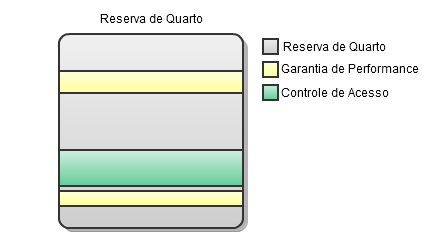
\includegraphics{img/context_aspect_concerns.png}
	\caption{Separação de interesses do módulo para reserva de quarto}\label{fig:context_aspect_concerns}
\end{figure}

No sistema de gerenciamento de hotel, é possível classificar reserva de quartos, \textit{check-in} e \textit{check-out} como interesses núcleo.
Os interesses de controle de acesso, acúmulo de pontos em um programa de fidelidade, controle de uma lista de espera, registro de mensagens e garantia
de \textit{performance} impactam diversas partes do sistema, por isso, são classificados como interesses entrecortantes. O interesse de controle de acesso deve 
verificar quais usuários podem acessar quais partes do sistema e, por isso, deve ser executado em todos os interesses núcleo. O interesse de
acúmulo de pontos em um programa de fidelidade impacta qualquer pagamento realizado. O interesse de controle de uma lista de espera impacta a
reserva de quartos. Já o registro de mensagens impacta grande parte dos interesses, pois as transações do sistema são registradas. Garantia de
\textit{performance} impacta todos os outros interesses, pois para garantir \textit{peformance} todo o sistema deve ser implementado com restrições
de segurança.

Utilizando os paradigmas convencionais para implementação de interesses, como a Programação Orientada a Objetos (POO), o módulo
para implementar o interesse de reserva de quartos seria composto  por código referente a reserva, e também a garantia de \textit{performance} e 
controle de acesso. A figura \ref{fig:context_aspect_concerns} mostra os interesses presentes no módulo de reserva de quartos. Observa-se a
implementação de vários interesses no mesmo módulo. Segundo Laddad\cite{Laddad:2003:AAP:993468}, essa situação é conhecida como \textbf{emaranhamento
de código} (\textit{code tangling}).

Outro sintoma de implementação deselegante de interesses é o \textbf{espalhamento de código} (\textit{code scattering}), quando o código 
referente a um mesmo interesse está disposto em diferentes módulos \cite{Laddad:2003:AAP:993468}. O espalhamento de código pode acontecer em duas
situações:

\begin{itemize}
  \item \textbf{Duplicação de código}: Diferentes módulos núcleo executam código
  referente a um mesmo interesse entrecortante.  
  
  Exemplo: Interesse para registro de informações (\textit{logging}) de um
  sistema; cada módulo núcleo contém chamadas a métodos da API
  de \textit{logging} para registrar informações.
  
  \item \textbf{Complementação de código}: Diferentes módulos executam código
  complementar para implementar um interesse entrecortante. 
  
  Exemplo: Interesse para autorização em um sistema; um módulo implementa o
  gerenciamento da sessão, outro módulo implementa o gerenciamento de
  permissões e controle de acesso e outro realiza a autenticação de usuários;
  cada módulo implementa uma parte do interesse de autorização.
\end{itemize}

O emaranhamento e espalhamento de código dificultam a manutenção de um sistema,
pois modificar um interesse impacta em modificar diferentes módulos. Além
disso, é complicado realizar um rastreamento entre interesses e módulos, pois o
código de um interesse está disposto em mais de um módulo. Outro problema é a
dificuldade de reuso de módulos devido a dependência de um módulo com vários
interesses \cite{Laddad:2003:AAP:993468}. 

\subsection{A necessidade de aspectos}

Os problemas destacados na sessão \ref{sec:concerns_abstraction} indicam a
necessidade de separação de interesses em diferentes módulos. A Programação Orientada a Aspectos 
(POA) \cite{Kiczales97aspect-orientedprogramming} é um paradigma de programação para representar
elegantemente os interesses de um sistema que impactam diversos módulos. 
Uma representação elegante de um interesse o separa em um único módulo e permite
o reuso entre diferentes aplicações. O objetivo da POA é a modularização dos interesses entrecortantes 
para que os mesmos fiquem separados dos módulos que implementam os interesses
núcleo da aplicação \cite{Laddad:2003:AAP:993468}.

É importante observar que, boa parte dos interesses de uma aplicação
são interesses núcleo e podem ser implementados elegantemente com a POO. Por
isso, a POA não pretende substituir a Programação Orientada a Objetos (POO), 
mas sim complementá-la com uma melhor representação para os interesses
entrecortantes.

\subsection{Metodologia de desenvolvimento}

Segundo \cite{Laddad:2003:AAP:993468}, para implementar um sistema utilizando aspectos
geralmente executam-se três fases:


\begin{enumerate}
  \item \textbf{Decomposição de Aspectos}: Identificação de quais requisitos são
  interesses núcleo e quais são interesses entrecortantes.
  \item \textbf{Implementação de Interesses}: Implementação de cada interesse
  separadamente.
  \item \textbf{Composição de Aspectos} (\textit{Weaving}): É a implementação de
  um aspecto para cada interesse entrecortante. O aspecto define o comportamento
  que será executado em determinados pontos de execução de um ou mais interesses. 
  Cada interesse entrecortante está contido em um único módulo: o aspecto. Após
  a implementação dos aspectos, se inicia o processo de composição \textit{weaving} 
  que insere o comportamento dos interesses entrecortantes nos interesses núcleo
  (nos pontos definidos nos aspectos). A figura \ref{fig:aspects_weaving} mostra
  o fluxo de desenvolvimento de uma aplicação orientada a aspectos.
\end{enumerate}

\begin{figure}[!hb]
	\centering
	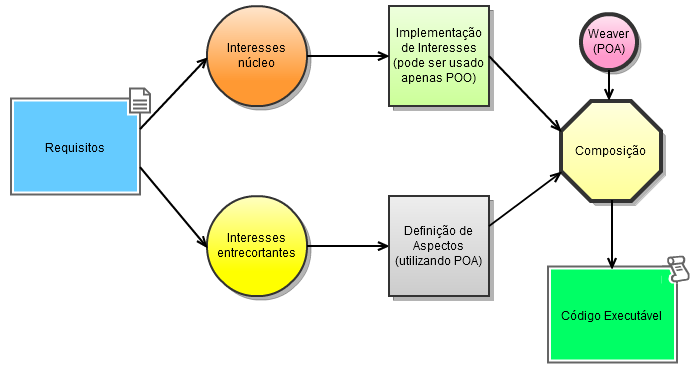
\includegraphics[scale=0.9]{img/aspects_weaving.png}
	\caption{Fluxo de desenvolvimento de uma aplicação com aspectos}\label{fig:aspects_weaving}
\end{figure}

\subsection{A linguagem AspectJ}

A linguagem AspectJ \cite{AspectJ11} é uma extensão da linguagem Java para programação orientada a aspectos. Qualquer programa implementado em Java
pode ser estendido utilizando AspectJ. A linguagem provê mecanismos para representar interesses entrecortantes e permite a composição dos mesmos com os interesses 
núcleo de um sistema. A linguagem oferece construções de extensão comportamentais e estáticas. As extensões comportamentais permitem que um novo
comportamento seja executado antes, durante ou depois de um determinado ponto de execução do sistema. As extensões estáticas permitem adicionar novos elementos na
estrutura das classes, por exemplo, a inserção de um novo método ou atributo. O conteúdo das próximas seções é baseado no guia de programação da
linguagem AspectJ \cite{aspectjguide} e no livro AspectJ: in Action \cite{Laddad:2003:AAP:993468}. Os exemplos, no entanto, são originais desta
dissertação.

\subsubsection{Construções Comportamentais}

Um dos principais conceitos comportamentais que devem ser compreendidos na linguagem é o de \textbf{ponto de junção}. Um ponto de junção é um
determinado ponto na execução de um programa. É importante observar que, um ponto de junção não é uma construção sintática de AspectJ, mas sim um conceito. 

A figura \ref{fig:aspects_join_point_model} descreve o fluxo de execução de um programa através da troca de mensagens entre diferentes objetos. Nesta
troca de mensagens existem diversos pontos de junção que podem ser capturados pela linguagem AspectJ. A seguir, será destacado cada ponto de junção
nesse fluxo de execução. No início da troca de mensagens, é chamado o método \textbf{umMetodo()} do \textbf{objetoA}. A chamada de um método em
AspectJ é representada pelo ponto de junção \textit{call}. Após a chamada do método, o código do mesmo será executado. A execução de um método é
representada pelo ponto de junção \textit{execution}. A duração de execução do método \textbf{umMetodo()} pode ser visualizada na ocorrência de
execução em azul. No início da execução de \textbf{umMetodo()}, realiza-se a chamada a \textbf{outroMetodo()}. A ocorrência de execução em verde
representa a duração da execução desse método. Dentro de \textbf{outroMetodo()} o método \textbf{metodoInterno()} é chamado. A ocorrência de execução em 
amarelo representa a duração de sua execução. Finalmente, instancia-se o \textbf{objetoC} através da chamada \textit{new}. A chamada de um construtor
também é um ponto de junção \textit{call} em AspectJ. A execução do mesmo pode ser capturada com o ponto de junção \textit{execution}. O tempo de
execução da instanciação desse construtor pode ser visualizado na ocorrência de execução em rosa. Os pontos de junção \textit{call} e
\textit{execution} são utilizados para capturar chamada e execução de métodos e construtores. 

\begin{figure}[!hb]
	\centering
	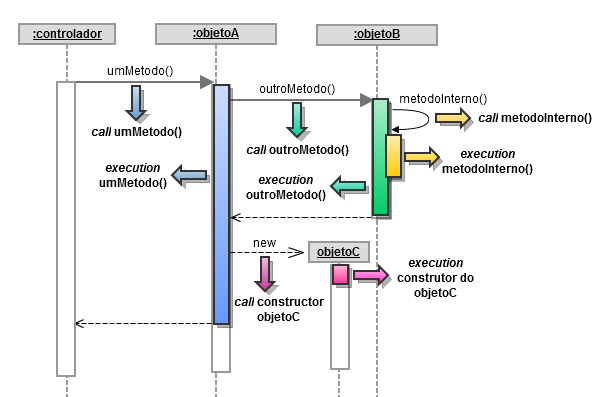
\includegraphics{img/aspects_join_point_model.png}
	\caption{Identificação de pontos de junção}\label{fig:aspects_join_point_model}
\end{figure}

É importante observar a diferença entre entre os pontos de junção de \textbf{chamada} (\textit{call}) e \textbf{execução} (\textit{execution}). Um
ponto de junção de chamada não está no código do método ou construtor sendo chamado, mas sim no código de quem está chamando o método ou construtor em
questão. Observe na figura \ref{fig:call_vs_execution} que a chamada (\textit{call}) ao método \textbf{umMetodo()} é realizada dentro do código
\textit{main} da aplicação. Já o ponto de junção de execução de um método ou construtor é disparado no corpo do método ou construtor em questão.
Observa-se na figura que a execução (\textit{execution}) do método \textbf{umMetodo()} refere-se à execução do código do próprio método.

\begin{figure}[!hb]
	\centering
	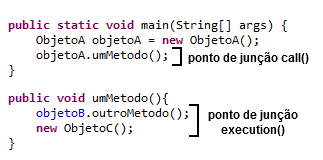
\includegraphics[scale=0.9]{img/call_vs_execution.png}
	\caption{Diferença entre os pontos de junção de chamada (call) e execução (execution)}\label{fig:call_vs_execution}
\end{figure}

O modelo de pontos de junção de AspectJ permite capturar também o tratamento de exceções, acesso e modificação de atributos (\textit{get} e
\textit{set}), inicialização e pré-inicialização de objetos, contexto de uma execução e execução de avisos. Estes pontos de junção também devem ser
representáveis em uma proposta para modelagem de programas orientados a aspectos.

Os pontos de junção em AspectJ definem quais são os pontos da execução de um programa possíveis de serem capturados. A linguagem deve disponibilizar
alguma construção sintática para selecionar pontos de junção. Para isso, AspectJ disponibiliza os \textbf{pontos de corte} (\textit{pointcuts}). Um
ponto de corte permite selecionar um conjunto de pontos de junção. 

Existem dois tipos de ponto de corte:

\begin{itemize}
  \item \textbf{Com nome}: Tem um nome e pode ser referenciado dentro de um
  aspecto.
  \item \textbf{Anônimo}: Não tem um nome e não pode ser referenciado dentro de
  um aspecto. Geralmente é definido dentro de um ponto de corte nomeado.
\end{itemize}

\begin{figure}[!hb]
	\centering
	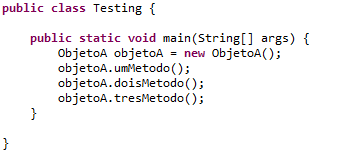
\includegraphics{img/pointcut_code.png}
	\caption{Exemplo de código em Java}\label{fig:pointcut_code}
\end{figure}

O código da figura \ref{fig:pointcut_code} mostra o exemplo de um simples código
em Java. É possível capturar pontos específicos da execução deste código
com pontos de corte. O ponto de corte \textbf{exemploDePontoDeCorte()} foi
definido para capturar chamadas ao método \textbf{umMetodo()} de objetos do tipo \textbf{ObjetoA}. 
Este ponto de corte é composto por dois pontos de corte anônimos e pode ser 
visualizado na figura \ref{fig:pointcut_vs_joinpoint}. O primeiro ponto de corte
anônimo seleciona um ponto de junção, capturando as chamadas ao método \textbf{umMetodo()} de 
objetos do tipo \textbf{ObjetoA}. O segundo ponto de corte anônimo seleciona vários
pontos de junção, pois captura qualquer chamada a membros (atributos, métodos,
construtores, etc) de objetos do tipo \textbf{ObjetoA}. 
É importante observar que, o segundo ponto de corte anônimo seleciona vários
pontos de junção em uma única definição. Entre os dois pontos de corte anônimos 
encontra-se o operador binário \textbf{\&\&}. Este operador especifica que o ponto de corte
\textbf{exemploDePontoDeCorte()} somente será satisfeito se \textbf{os dois
pontos de corte anônimos forem satisfeitos}. Assim, o ponto de corte
\textbf{exemploDePontoDeCorte()} seleciona apenas um ponto de junção: execução da
chamada ao método \textbf{umMetodo()} com o método membro de um objeto do
tipo \textbf{ObjetoA}. A captura de um único método pode ser visualizada no
código na parte inferior da figura \ref{fig:pointcut_vs_joinpoint}
(método selecionado está destacado com uma flecha laranja).

\begin{figure}
	\centering
	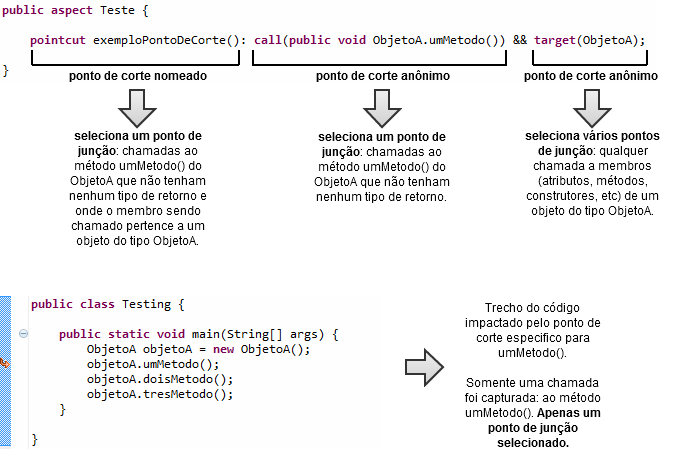
\includegraphics{img/pointcut_vs_joinpoint.png}
	\caption{Exemplo de ponto de corte}\label{fig:pointcut_vs_joinpoint}
\end{figure}

Para possibilitar a captura de vários pontos de junção em um mesmo ponto de
corte de maneira praticável, AspectJ disponibiliza os \textbf{wildcards}. 
Um \textit{wildcard} é semelhante a uma expressão regular. As seguintes notações
estão disponíveis na definição de \textit{wildcards}:

\begin{itemize}
  \item * representa qualquer número de caracteres, exceto pontos.
  \item .. representa um ou mais caracteres, incluindo qualquer número de
  pontos.
  \item + representa uma subclasse ou sub-interface de um dado tipo.
\end{itemize}

Utilizando \textit{wildcards} é possível modificar o ponto de corte especificado na figura \ref{fig:pointcut_vs_joinpoint} para que capture chamadas
para qualquer método pertencente a objetos do tipo \textbf{ObjetoA}. Para isso, modifica-se o primeiro ponto de corte anônimo, substituindo
\textbf{umMetodo()} pela notação \textbf{*}, capturando agora todos os métodos do ObjetoA, independente do nome. Além disso, adiciona-se a 
notação \textbf{..}, capturando métodos com qualquer número de parâmetros. 

\begin{figure}
	\centering
	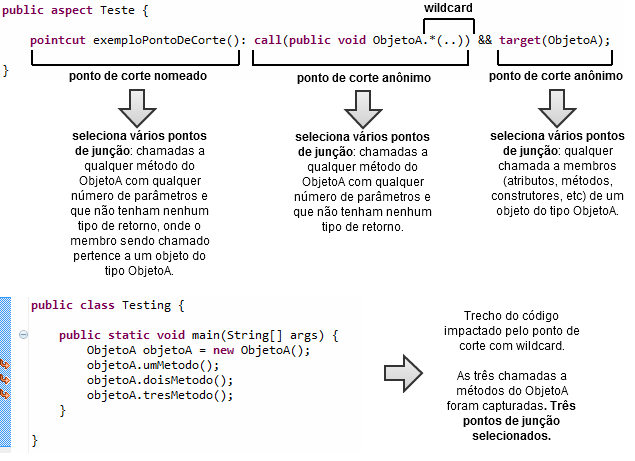
\includegraphics{img/pointcut_vs_joinpoint_wildcard.png}
	\caption{Exemplo de ponto de corte utilizando wildcards}\label{fig:pointcut_vs_joinpoint_wildcard}
\end{figure}

A figura \ref{fig:pointcut_vs_joinpoint_wildcard} mostra o ponto de corte redefinido, utilizando \textit{wildcards}. 
O novo ponto de corte captura a chamada de qualquer método, com qualquer número
de parâmetros e qualquer tipo de retorno de um objeto do tipo \textbf{ObjetoA}.
A captura de todos os métodos pode ser visualizada no código da parte inferior
da figura \ref{fig:pointcut_vs_joinpoint} (métodos selecionados estão destacados
com flechas laranjas). O ponto de corte da figura \ref{fig:pointcut_vs_joinpoint_wildcard} captura três pontos de junção.

Os pontos de corte das figuras \ref{fig:pointcut_vs_joinpoint} e \ref{fig:pointcut_vs_joinpoint_wildcard} foram definidos utilizando \textbf{padrões
de assinatura} (\textit{signature patterns}). Um padrão de assinatura é utilizado para especificar quais assinaturas de um programa em Java serão capturadas. No
exemplo de ponte de corte da figura \ref{fig:pointcut_vs_joinpoint}, a assinatura \textbf{public void ObjetoA.umMetodo()} permite capturar as chamadas
ao método \textbf{umMetodo()} do \textbf{ObjetoA} sem retornar nenhum objeto. Já a assinatura \textbf{public void ObjetoA.*(..)} da 
figura \ref{fig:pointcut_vs_joinpoint_wildcard} permite capturar as chamadas a qualquer método, com qualquer número de parâmetros e sem nenhum
tipo de retorno do \textbf{ObjetoA}. AspectJ disponibiliza padrões de assinatura para especificar pontos de corte para capturar métodos, construtores,
tipos, exceções, atribuições, etc. Os seguintes padrões de assinatura estão disponíveis:

\begin{itemize}
  \item \textbf{Assinaturas de Tipo} (\textit{AssinaturaDeTipo}): Permite
  capturar definições de classes e interfaces. É possível especificar o pacote e o nome
  do tipo a ser capturado.
  \item \textbf{Assinaturas de Método e Construtores}
  (\textit{AssinaturaDeMetodo} e \textit{AssinaturaDeConstrutor}): Permite
  capturar métodos e construtores. É possível especificar escopo, tipo de retorno, localização e nome do método
  ou construtor e tipos de argumentos.
  \item \textbf{Assinaturas de Atributos} (\textit{AssinaturaDeAtributo}):
  Permite capturar definições de atributos de classes. É possível especificar o escopo, tipo do
  atributo, localização e nome do atributo.
\end{itemize}

A figura \ref{fig:signatures} mostra exemplos de padrões de assinatura na captura de pontos de junção. O primeiro exemplo mostra o uso de um padrão de
método para capturar chamadas ao método \textbf{umMetodo()} de objetos do tipo \textbf{ObjetoA} que não tenha retorno e com escopo público. O segundo
exemplo mostra o padrão de tipo para capturar objetos do tipo \textbf{ObjetoA}. O terceiro mostra o padrão de atributo para capturar atribuições ao
atributo \textbf{name} de objetos do tipo \textbf{ObjetoB}, em qualquer o escopo. O último exemplo apresenta o padrão de construtor para capturar a
inicialização de objetos do tipo \textbf{ObjetoA} sem nenhum parâmetro. Além do operador \textbf{\&\&}, que tem a semântica do operador lógico do tipo
AND, AspectJ disponibiliza outros operadores binários. O operador \textbf{||} tem a mesma semântica de um operador lógico do tipo OR e o operador
\textbf{!} possui a mesma semântica do operador lógico do tipo NOT.

\begin{figure}[!hb]
	\centering
	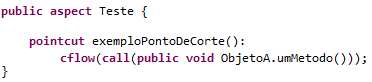
\includegraphics{img/flow_p1.png}
	\caption{Ponto de corte para captura do fluxo de execução inclusivo: cflow()}\label{fig:flow_p1}
\end{figure}

\begin{figure}[!hb]
	\centering
	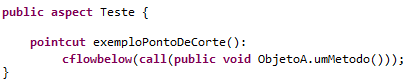
\includegraphics{img/flow_p2.png}
	\caption{Ponto de corte para captura do fluxo de execução exclusivo: cflowbelow()}\label{fig:flow_p2}
\end{figure}
 
Além dos pontos de corte para captura de execução, chamada, tratamento de exceção e atribuição, existem pontos de corte mais complexos relativos ao
fluxo de execução de um programa. Os \textbf{pontos de corte para captura do fluxo de execução} capturam todos os pontos de junção a partir de um outro ponto de
corte. Existem dois tipos: \textit{cflow(PontoDeCorte)} e \textit{cflowbelow(PontoDeCorte)}. O ponto de corte da figura \ref{fig:flow_p1}
é do tipo \textit{cflow()} e captura todos os pontos de junção disparados a partir do ponto de corte \textbf{call(public void ObjetoA.umMetodo())},
inclusive a chamada ao próprio método. O ponto de corte da figura \ref{fig:flow_p2} é do tipo \textit{cflowbelow()} e captura os mesmos pontos de
junção do anterior, exceto a chamada ao próprio método.

\begin{figure}[!htb]
	\centering
	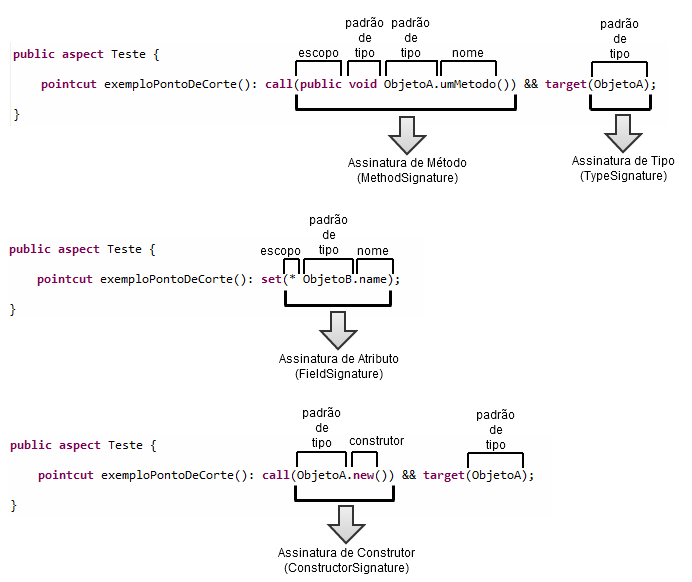
\includegraphics[scale=0.9]{img/signatures.png}
	\caption{Exemplo de assinaturas em AspectJ}\label{fig:signatures}
\end{figure}

Existem também \textbf{pontos de corte baseados na estrutura léxica do código}. Estes pontos de corte capturam pontos de junção que ocorrem dentro de
um determinado trecho de código. Existem dois tipos: \textit{within(AssinaturaDeTipo)} e \textit{withincode(AssinaturaDeConstrutor ou
AssinaturaDeMétodo)}. O primeiro tipo captura os pontos de junção que ocorrerem dentro de classes, aspectos ou classes aninhadas de um determinado
tipo (\textit{AssinaturaDeTipo}. O segundo tipo captura os pontos de junção que estiverem dentro do código de um dado método ou construtor
(\textit{AssinaturaDeConstrutor ou AssinaturaDeMetodo}). 

Outros tipos de \textbf{ponto de corte permitem capturar o contexto de uma
execução}. O ponto de corte \textit{this(TipoDoObjeto)} permite capturar todos
os pontos de junção onde o objeto que está executando é do tipo
\textit{TipoDoObjeto}. Já o ponto de corte \textit{target(TipoDoObjeto)} permite
capturas os pontos de junção onde o objeto que está sendo chamado é do tipo
\textit{TipoDoObjeto}. Estes pontos de corte permitem passar o contexto de uma execução, isto é, instâncias de objetos, para um aviso,
o que será abordado ainda neste capítulo. 

Existem também os \textbf{pontos de corte para argumentos}.
Estes pontos de corte tem a seguinte sintaxe: \textit{args(AssinaturaDeTipo, 
\ldots , AssinaturaDeTipo)}. Eles permitem capturar pontos de junção
baseados nos argumentos recebidos. Por exemplo, capturar os métodos 
que recebam três atributos do tipo \textit{String}.

Após identificar quais pontos de junção serão capturados através de pontos de
corte, deve-se especificar qual o comportamento que será executado antes, 
durante ou depois dos locais selecionados. Para isso, AspectJ propõe uma
construção denominada \textbf{aviso}. Um aviso é uma construção parecida com um método
em Java. Ele define um comportamento para ser executado. Existem três tipos de
avisos:

\begin{itemize}
  \item \textbf{Antes} (before): Executa antes do ponto de junção capturado.
  \item \textbf{Depois} (after): Executa depois do ponto de junção capturado.
  Existe uma variação ao aviso \textit{after} que executará apenas se o ponto de
  junção capturado não lançar nenhuma exceção, isto é, só será executado se a execução
  do ponto de junção tiver sucesso. Esse tipo de aviso é denominado
  \textit{after returning}.
  \item \textbf{Durante} (around): É o tipo de aviso mais poderoso, pois
  pode executar no lugar do ponto de junção capturado, continuar a execução
  original ou alterar o contexto de execução.
\end{itemize}

A figura \ref{fig:advice_code} mostra um exemplo de um aviso que executa
\textbf{depois}(\textit{after}) do ponto de corte
\textbf{exemploDePontoDeCorte()}. Este aviso recebe o contexto da execução
como parâmetro (um objeto do tipo \textbf{ObjetoA}) e imprime uma
mensagem com a representação textual deste objeto. O corpo deste aviso é o
trecho de código que realiza a impressão da representação do objeto. Em AspectJ,
o corpo de um aviso pode conter qualquer código Java. Observa-se também que o
objeto passado no contexto de execução é referenciado no corpo do aviso. Os
pontos de corte \textit{target()} e \textit{this()} são muito utilizados, pois
permitem passar o contexto de execução para um aviso.

\begin{figure}[!hb]
	\centering
	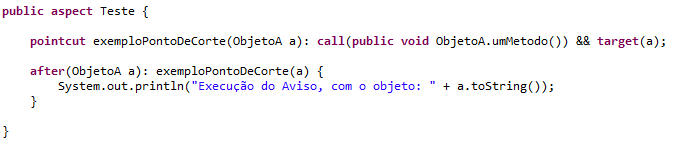
\includegraphics[scale=0.9]{img/advice_code.png}
	\caption{Exemplo de aviso com contexto de execução}\label{fig:advice_code}
\end{figure}

\subsubsection{Construções Estáticas}

Uma das construções estáticas propostas por AspectJ é a \textbf{introdução}, que
permite alterar a estrutura de classes, aspectos e interfaces adicionando novos
métodos e atributos. A figura \ref{fig:introduction} mostra um aspecto que
introduz o método \textbf{metodoIntroduzido()} e os atributos
\textbf{atributoUm} e \textbf{atributoDois} na classe do tipo \textbf{ObjetoA}.
Os dois atributos introduzidos são utilizados no próprio método
\textbf{metodoIntroduzido()}. Isto é possível, pois
o compilador AspectJ sabe que o método introduzido pertence ao \textbf{ObjetoA}
e o objeto que executará este método será um objeto do tipo \textbf{ObjetoA}.

\begin{figure}
	\centering
	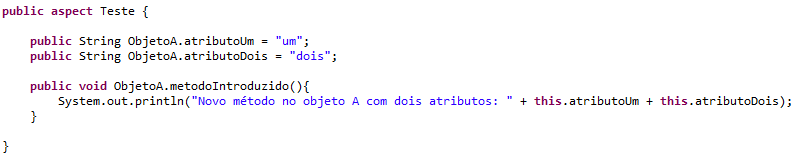
\includegraphics[scale=0.9]{img/introduction.png}
	\caption{Introdução de métodos e atributos}\label{fig:introduction}
\end{figure}

Outra funcionalidade disponível na linguagem é a \textbf{modificação da hierarquia de classes}, permitindo a definição de
relacionamentos de herança, implementação de interfaces, dentre outras
alterações \cite{Laddad:2003:AAP:993468}. O exemplo da figura
\ref{fig:introduction_interface} mostra a introdução de um relacionamento de
herança entre as classes \textbf{ObjetoA} e \textbf{ObjetoB}.

\begin{figure}
	\centering
	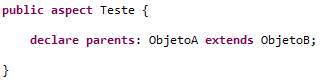
\includegraphics{img/introduction_interface.png}
	\caption{Introdução de relacionamentos de herança}\label{fig:introduction_interface}
\end{figure}

\subsubsection{Aspecto}

Resumidamente, para estender um sistema utilizando Java com AspectJ, deve-se
identificar os pontos de junção que serão selecionados por um ponto de corte e
implementar o aviso que introduzirá o novo comportamento antes, durante ou
depois do ponto de corte. O elemento da linguagem que agrupa todas essas
construções é o \textbf{aspecto}. Um aspecto é uma unidade de modularização 
semelhante a uma classe, mas com diferenças em relação ao ciclo de vida, pois
não pode ser instancializado e não pode especializar de um outro aspecto concreto.
No entanto, um aspecto pode ser declarado como abstrato e aspectos concretos
podem estendê-lo para implementar suas declarações abstratas.

\subsubsection{Exemplo de Aspecto}

O objetivo deste exemplo é utilizar a linguagem AspectJ para implementar de maneira elegante o padrão de projeto \textbf{Observador}
\cite{Gamma:1995:DPE:186897}. Este padrão permite que um ou mais objetos se cadastrem para escutar mudanças de um outro objeto. A implementação do padrão está 
presente nos exemplos da IDE para desenvolvimento com aspectos: AspectJ Development Tools (AJDT) \cite{AspectJ11}.

Um dos requisitos deste padrão é que um ou mais objetos (observadores) possam
escutar mudanças de um outro objeto (sujeito) e serem atualizados. Assim,
identificam-se duas interfaces: \textit{Subject} e \textit{Observer}. A interface \textit{Subject}
deve armazenar seus observadores e prover métodos para adicionar, remover e obter
os mesmos. A interface \textit{Observer} deve prover métodos para associar e
obter o sujeito observado. Esses requisitos são implementados no aspecto como
introduções de métodos e atributos. O trecho de código da figura \ref{fig:aspects_observer_1} apresenta as introduções realizadas. Observa-se a
introdução do atributo \textit{observers} e dos métodos \textit{addObserver()},
\textit{removeObserver()} e \textit{getObservers()} na interface
\textit{Subject}. Na interface \textit{Observer} foram introduzidos os métodos
\textit{setSubject()} e \textit{getSubject()} e o atributo
\textit{subject}.

Além de introduzir os métodos e atributos para permitir a associação entre
sujeitos e observadores, deve-se implementar a lógica que capture mudanças nos
sujeitos e avise os observadores. Essa lógica pode ser implementada com o uso de
pontos de corte e avisos. O ponto de corte \textit{stateChanges()} é
responsável por escutar mudanças em um sujeito e após (\textit{after}) cada
mudança, um aviso é executado para atualizar os observadores. O ponto de corte
\textit{stateChanges()} deve ser abstrato, pois este ponto de corte será
diferente para cada sujeito a ser observado. O trecho de código que implementa o
ponto de corte e o aviso também pode ser visualizado na figura \ref{fig:aspects_observer_1}.

Com esses requisitos implementados, é possível juntar os dois trechos de código
em um aspecto abstrato que implementa o padrão \textbf{Observador}. Este aspecto
é abstrato, pois tem o ponto de corte abstrato \textit{stateChanges()}, que deve
ser definido por um aspecto concreto, selecionando quais pontos de junção serão
capturados para definir que uma mudança ocorreu. O aspecto abstrato recebe o
nome de \textit{SubjectObserverProtocol} e pode ser visualizado na figura
\ref{fig:aspects_observer_1}. Um desenvolvedor que deseja utilizar o padrão de projeto
observador pode reusar o aspecto abstrato \textit{SubjectObserverProtocol}, 
estendendo-o com a implementação de um aspecto concreto. Este aspecto concreto
deve especificar qual classe faz o papel de sujeito, isto é, qual classe
implementa a interface \textit{Subject} e qual classe faz o papel de
observador, isto é, qual classe implementa a interface \textit{Observer}.
Além disso, deve definir o ponto de corte \textit{stateChanges()}, para
especificar em quais pontos de junção serão detectadas mudanças. 

\begin{figure}
	\centering
	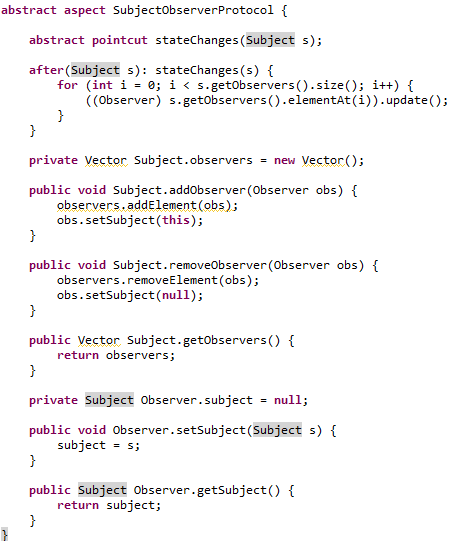
\includegraphics{img/aspects_observer_1.png}
	\caption{Aspecto abstrato para implementação do padrão de projeto Observador}\label{fig:aspects_observer_1}
\end{figure}

Considerando como exemplo um sistema de interface gráfica com um botão e um
texto com cor variável. Define-se como requisito que a cor deste texto deve modificar toda vez
que o botão foi clicado. Este requisito pode ser implementado utilizando o
aspecto abstrato. O pequeno sistema de interface gráfica contém a classe
\textit{Button} representando o botão e a classe \textit{ColorLabel}
representando o texto com cor. A classe \textit{Button} é o sujeito observado,
por isso implementa a interface \textit{Subject}. O observador é a classe
\textit{ColorLabel} que implementa a interface \textit{Observer}. Além disso,
introduz-se o método \textit{update()} na classe \textit{ColorLabel} para
atualizar a cor do texto quando houver alguma mudança no botão. O que está
faltando definir é quais pontos na execução do programa geram mudanças no botão.
Estes pontos são definidos ao implementar o ponto de corte abstrato
\textit{stateChanges()}. Define-se que serão capturadas as chamadas ao método
\textit{click()} da classe \textit{Button}, onde o objeto alvo é do tipo
\textit{Subject} (neste caso é da classe \textit{Button}, pois esta classe
implementa \textit{Subject}. O código do aspecto concreto para implementar o
padrão observador pode ser visualizado na figura \ref{fig:aspects_observer_2}. 
Este aspecto captura cliques em um botão, atualizando a cor de um texto.

\begin{figure}
	\centering
	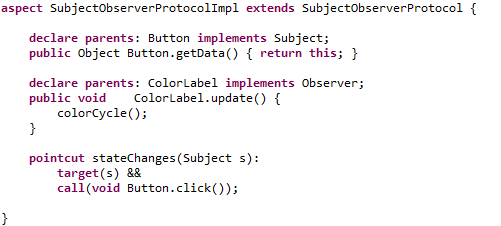
\includegraphics{img/aspects_observer_2.png}
	\caption{Aspecto concreto implementando o padrão de projeto Observador em um sistema de
	interface gráfica}\label{fig:aspects_observer_2}
\end{figure}

\section{Análise e Projeto com UML}

A análise e projeto de sistemas orientados a objetos é uma abordagem utiliza no desenvolvimento de aplicações complexas. 
Aplicações complexas necessitam de um planejamento antes da implementação. Usualmente divide-se o desenvolvimento de
um sistema em quatro fases: análise, projeto, implementação e testes
\cite{pressman:01}. As fases de análise e projeto são as fases aonde realiza-se 
a maior parte do planejamento de um desenvolvimento. Já as fases de
implementação e testes são responsáveis pela codificação com o objetivo de obter
um programa executável e que cumpra os requisitos do cliente. 

Nas fases de análise e projeto utilizam-se modelos que permitem representar o
sistema em diferentes níveis de abstração, facilitando a compreensão e reduzindo
a complexidade. A fase de análise tem como objetivo compreender os principais conceitos
do domínio do problema, evitando o uso de termos computacionais. Já a fase de
projeto foca na solução que será desenvolvida para produzir um sistema a partir
da compreensão do problema. 

\subsection{Múltiplos pontos de vista de um sistema}

Segundo \cite{silva:07}, um sistema orientado a objetos pode ser visualizado por
diferentes pontos de vista:

\begin{itemize}
  \item Estrutural de sistema: Essa visão contém o conjunto de elementos de um
  sistema orientado a objetos e seus relacionamentos.
  \item Estrutural de classe: Essa visão contém o detalhamento da estrutura de
  cada um dos elementos de um sistema.
  \item Comportamental de sistema: Essa visão permite compreender o
  conjunto de funcionalidades do sistema e como os elementos iteragem em tempo
  de execução.
  \item Comportamental de classe: Essa visão permite compreender o comportamento
  de um elemento isoladamente. Geralmente compreende-se a variação de estados
  desse elemento.
\end{itemize}
  
Uma modelagem que permita representar esses quatro pontos de vista pode ser considerada completa. Uma \textbf{modelagem completa} fornece subsídios
para a geração de código e facilita a compreensão e manutenção de um sistema. 

\section{UML: Segunda Versão}

A segunda versão da UML \cite{uml:05} permite representar o comportamento e a estrutura de um sistema nas fases de análise e projeto
através de diagramas estruturais e comportamentais. Esta linguagem é um padrão da \textit{Object Management Group} (OMG)\sigla{OMG}{Object Management
Group}, por isso é compreendida e utilizada por grande parte dos desenvolvedores e analistas para realizar a modelagem de sistemas. Os
diagramas da segunda versão da UML permitem a representação dos quatro pontos de vista essenciais para programas  orientados a objetos. As seções que tratam dos diagramas estruturais e
comportamentais da UML são baseadas no conteúdo do livro UML 2 em Modelagem Orientada a Objetos \cite{uml2ricardo:03} e no Tutorial de UML da Sparx
Systems \cite{sparx_tutorial}.

\subsection{Diagramas Estruturais}

A segunda versão da UML disponibiliza sete diagramas estruturais: diagrama de classes, componentes, estrutura composta, instalação, objetos,
pacotes e perfil. Os diagramas estruturais utilizados nesta dissertação são os diagramas de classe e o diagrama de perfil. Este último foi
introduzido na versão 2.2 da linguagem e é utilizado para a extensão da linguagem para um domínio específico.

\subsubsection{Diagrama de Classes}

O diagrama de classes permite representar a estrutura e os relacionamentos dos elementos de um sistema. Este diagrama permite visualizar o sistema
como um todo, visualizando os relacionamentos entre os elementos e também permite visualizar a estrutura de cada elemento, com seus atributos e
métodos. Os principais componentes deste diagrama são as classes, associações, atributos, métodos e pacotes.

\subsubsection{Diagrama de Perfil}

O diagrama de perfil permite estender o modelo da linguagem para representar conceitos de um determinado domínio de aplicações. Um perfil é composto
por \textbf{estereótipos}, \textbf{restrições} e \textbf{valores rotulados}. 

Um \textbf{estereótipo} adiciona uma semântica adicional a um elemento da UML. Geralmente adiciona-se um estereótipo para diferenciar os papéis dos
elementos de um modelo. Por exemplo, a classe \textit{RoomManager} da figura \ref{fig:stereotype_1} foi associada ao estereótipo \textit{Controller} 
para representar que esta classe tem o papel de controlador. É possível adicionar mais de um estereótipo a mesma classe. A classe
\textit{ReservationManager} é associada aos estereótipos \textit{Controller} e \textit{Client} para representar que esta classe é
um controlador e que encontra-se do lado do cliente. Os estereótipos \textit{Client} e \textit{Controller} estendem o elemento do 
meta-modelo da UML \textit{Class}, podendo assim ser aplicados a qualquer classe.  É importante observar que um estereótipo pode ser associado a
qualquer elemento do meta-modelo da UML. O atributo \textit{id} da classe \textit{Room} está associado ao estereótipo \textit{key} para representar
que este atributo define unicamente uma sala. O estereótipo \textit{key} está estendendo o meta-modelo da UML \textit{Attribute}.

\begin{figure}
	\centering
	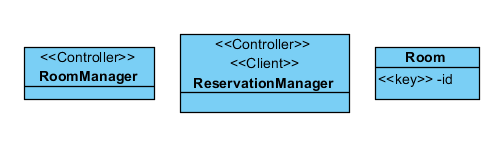
\includegraphics{img/stereotype_1.png}
	\caption{Uso de estereótipos em um diagrama de classes}\label{fig:stereotype_1}
\end{figure}

Um estereótipo adiciona um papel a um elemento do modelo. Para adicionar mais informações a um elemento, podem-se definir \textbf{valores rotulados}.
A linguagem permite associar zero ou mais valores rotulados a um estereótipo. Um valor rotulado pode ser um elemento do modelo, um número, um texto, um booleano ou uma 
enumeração definida pelo usuário. Ao utilizar um estereótipo em um modelo, deve-se definir os valores rotulados associados ao mesmo. Os valores
rotulados adicionam uma semântica ao estereótipo. O exemplo da figura \ref{fig:tagged_values_1} contém duas classes que representam sistemas
operacionais: \textit{Fedora64} e \textit{WindowsXP}. Estas classes são marcadas com o estereótipo \textit{Operating System}. Este estereótipo 
exige a definição do valor rotulado \textit{platfom}, que define qual a plataforma do sistema operacional. Este valor rotulado é um enumerado com dois
tipos: x86 e x64. No exemplo, a classe \textit{Fedora64} associa o valor x64 ao valor rotulado \textit{platform}, pois é um sistema de 64 bits. Já a classe
\textit{WindowsXP} associa o valor x86 ao mesmo valor rotulado, pois é um sistema de 32 bits. Finalmente, \textbf{restrições} podem ser
introduzidas ao modelo para garantir a consistência no próprio modelo e nos seus relacionamentos.

\begin{figure}
	\centering
	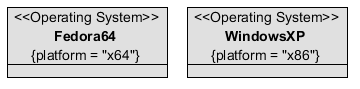
\includegraphics{img/tagged_values_1.png}
	\caption{Uso de valores rotulados em um diagrama de classes}\label{fig:tagged_values_1}
\end{figure}

A figura \ref{fig:profile_diagram} mostra a definição de um perfil UML para modelagem de sistemas que desejam representar veículos
\cite{VisualParadigm11}. Foram definidos sete estereótipos que estendem o elemento do meta-modelo \textit{Class}. Observa-se a generalização entre os
estereótipos \textit{Vehicle}, \textit{Mini}, \textit{Pickup Truck} e \textit{Convertible}. O estereótipo \textit{Pickup Truck} especializa o
estereótipo \textit{Vehicle}. O relacionamento de composição entre os estereótipos \textit{Interior} e \textit{Seat} define que o interior de um
veículo deve ter no mínimo um assento. Observa-se também a presença de dois valores rotulados do tipo texto no estereótipo \textit{Seat}:
\textit{texture} e \textit{pattern}. Existem outros valores rotulados neste perfil como: o limite de passageiros (\textit{passenger-limit}) no
estereótipo \textit{Vehicle}, que é do tipo inteiro; o limite de velocidade (\textit{speed-limit}) também no estereótipo \textit{Vehicle}, que é do
tipo ponto flutuante, dentre outros. Este perfil pode ser exportado no formato \textit{XML Metadata Interchange} (XMI)\sigla{XMI}{XML Metadata Interchange} \cite{xmi:11} 
e utilizado por outras ferramentas do tipo \textit{Computer Aided Software Engineering} (CASE)\sigla{CASE}{Computer Aided Software Engineering}. Assim, 
é possível intercambiar perfis entre diferentes ferramentas CASE. A vantagem do intercâmbio de perfis é o reuso de
especificações já prontas sobre um determinado domínio de aplicação. Um exemplo de perfil que pode ser reusado por outros desenvolvedores é um perfil
que especifique sistemas orientados a aspectos.

\begin{figure}
	\centering
	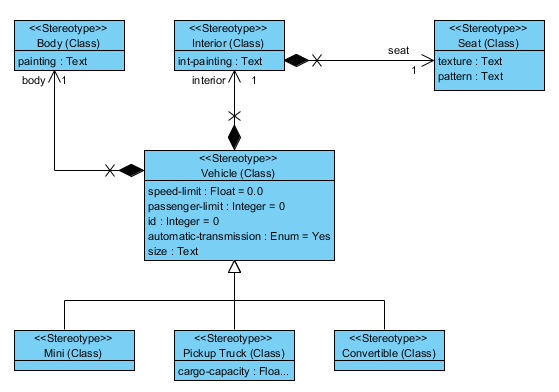
\includegraphics{img/profile_diagram.png}
	\caption{Diagrama de Perfil para representar veículos}\label{fig:profile_diagram}
\end{figure}

\subsection{Diagramas Comportamentais}

A segunda versão da UML possui sete diagramas comportamentais: diagrama de atividades, máquina de estados, casos de uso, comunicação, visão geral de 
interação, sequência e de tempo. Neste trabalho serão utilizados os diagramas de máquina de estados e de sequência.

\subsubsection{Diagrama de Máquina de Estados}

O diagrama de máquina de estados representa os estados e o comportamento de um objeto, especificando a sequência de eventos que um objeto recebe
durante sua existência. Os principais componentes deste diagrama são os estados e as transições. Um diagrama de máquina de estados também pode
representar concorrência utilizando nodos \textit{fork} e \textit{join} com regiões concorrentes. Este mecanismo permite realizar a sincronização
entre diferentes estados. Na POO utiliza-se o diagrama de máquina de estados para especificar os diferentes estados de uma classe.
Neste caso, cada estado representa uma configuração dos atributos da classe. As transições são as execuções de métodos, que modificam valores de
atributos, evoluindo a classe para um novo estado.

\subsubsection{Diagrama de Sequência}

O diagrama de sequência representa as trocas de mensagens entre objetos. Este diagrama permite compreender a interação entre objetos com
foco no tempo e na ordem das mensagens durante uma execução. Os principais componentes do diagrama de sequência são as linhas de vida de objetos, as
mensagens e os fragmentos combinados. Um fragmento combinado permite adicionar condições e iterações em uma troca de mensagens. Outro componente
utilizado nesta dissertação é a invariante de estado, que permite estabelecer uma condição para que um conjunto de mensagens seja executado. Este conjunto de mensagens somente será executado quando o sistema atingir o estado associado com a invariante de estado. O comportamento
de cada caso de uso pode ser refinado com um diagrama de sequência.

\section{Model-Driven Engineering}

O aumento da complexidade das plataformas mais utilizadas no desenvolvimento de software (CORBA, J2EE, .NET) gera um grande esforço para
desenvolvedores portarem código de aplicação para estas plataformas \cite{Schmidt:2006:GEI:1115688.1115706}. A manutenção do código das aplicações e
das plataformas ainda é realizada utilizando linguagens de programação tradicionais, como Java e C++. A complexidade destas plataformas implementadas
com linguagens tradicionais dificulta a obtenção de uma visão unificada, que facilite a compreensão do impacto de uma mudança no sistema.

Model-Driven Engineering (MDE) \sigla{MDE}{Model-Driven Engineering} é uma metodologia de desenvolvimento de software focada na representação de
elementos de um domínio de problema em nível de modelo. Esta metodologia surgiu com o objetivo de permitir uma melhor representação destas plataformas
complexas. A técnica de MDE utiliza meta-modelagem para representar o domínio de uma aplicação, definindo os relacionamentos entre os conceitos do
sistema. Através da meta-modelagem, define-se uma linguagem específica para um determinado domínio, que pode ser reusada. A partir desta linguagem,
independente de plataforma, é possível utilizar um transformador que transforma os modelos em uma linguagem alvo.

A metodologia de MDE tem um futuro promissor, pois permite diminuir a complexidade na representação de conceitos de um domínio de aplicação
ou de uma plataforma. A linha de aprendizado de um sistema modelado com a técnica de MDE é menor do que com modelagem tradicional (somente UML) ou com
linguagens tradicionais. A manutenabilidade do sistema também é facilitada utilizando MDE.

\section{Meta-modelagem}

Uma linguagem geralmente é definida através de uma gramática na forma \textit{Backus Naur Form} (BNF) \sigla{BNF}{Backus Naur Form}. Uma linguagem
bem definida pode ser interpretada de forma automatizada por um computador. Este método de definição de linguagens é utilizado até hoje para
representar linguagens baseadas em texto. Para facilitar a definição de linguagens para modelagem pode-se utilizar um outro mecanismo. Este mecanismo
é denominado \textbf{meta-modelagem}, que permite a descrição de uma linguagem na forma de um modelo \cite{mda:03}. Um meta-modelo de uma linguagem define os 
elementos que podem ser utilizados na criação de modelos utilizando esta linguagem. Considerando a UML como exemplo, o meta-modelo da linguagem define
elementos como Classe, Estado, Pacote, Operação, etc. Assim, um modelo definido utilizando UML pode definir instâncias de classes, estados, pacotes, operações, etc. 
A OMG define uma arquitetura em quatro camadas para representar os modelos padrões para definição de modelos. Esta arquitetura pode ser visualizada
na figura \ref{fig:omg_meta_model}. 

Na arquitetura da figura \ref{fig:omg_meta_model}, o modelo M3 define elementos que podem ser utilizados para representar conceitos no modelo M2. O
modelo M3 é considerado o meta-meta-modelo da OMG. O \textit{Meta-Object Facility} (MOF) \sigla{MOF}{Meta-Object Facility}) é um padrão da OMG que define a linguagem que
deve ser utilizada para definir linguagens para modelagem \cite{mof:11}. O MOF está no nível M3. O modelo M2 especifica os elementos que podem ser
utilizados no modelo M1. Um modelo no nível M2 é denominado um meta-modelo. Linguagens geralmente são definidas neste nível de modelo. Observa-se na
figura \ref{fig:omg_meta_model} a definição de uma classe (\textit{UML Class}) e de um atributo (\textit{UML Attribute}) no nível M2. Estes elementos
fazem parte da definição do meta-modelo da UML. O modelo M1 contém instâncias de elementos definidos no modelo M2. Este modelo é o que é definido
pelo analista ao realizar a modelagem de um determinado sistema com UML. Na figura \ref{fig:omg_meta_model} observa-se a definição de duas classes:
\textit{Customer} e \textit{Order} no nível M1. Além disso, definem-se os atributos \textit{title}, \textit{name} e \textit{number} nessas classes. As
classes são instâncias da meta-classe \textit{UML Class}. Os atributos são instâncias da meta-classe \textit{UML Attribute}. Finalmente, o modelo M0
representa as instâncias de um sistema representadas em um modelo. Um exemplo de instância é um cliente do tipo \textit{Customer} com o nome
\textit{Joe Nobody}.

\begin{figure}
	\centering
	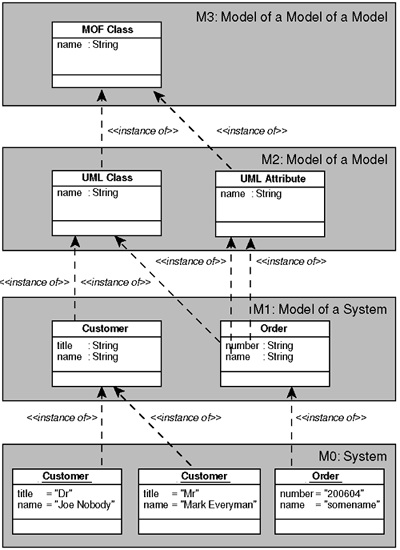
\includegraphics{img/omg_meta_model.png}
	\caption{Meta-modelo da Object Management Group (OMG)}\label{fig:omg_meta_model}
\end{figure}

O meta-modelo da UML é definido no nível M2 a partir do MOF. Este meta-modelo é uma instância do MOF. Uma parte do meta-modelo pode ser visualizada na
figura \ref{fig:uml_meta_model}. Esta parte do modelo define os componenentes para representar classes, atributos, operações, etc.

\begin{figure}
	\centering
	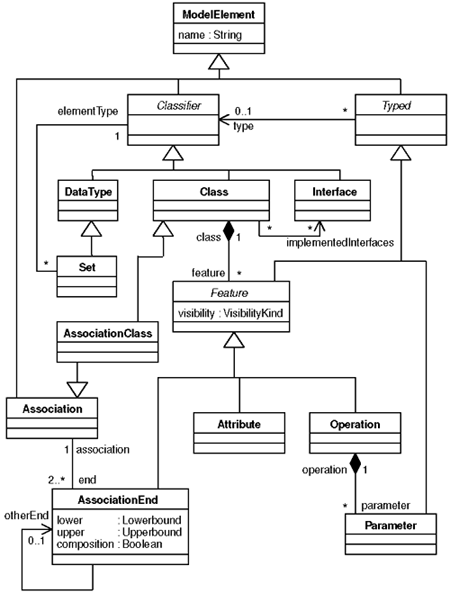
\includegraphics{img/uml_meta_model.png}
	\caption{Meta-modelo da UML}\label{fig:uml_meta_model}
\end{figure}

É importante observar no modelo da figura \ref{fig:uml_meta_model} que qualquer elemento de um modelo da UML deve derivar de \textit{ModelElement} e
por isso deve ter um nome. Nota-se também a presença de Classe (\textit{Class}), Atributo (\textit{Attribute}) e Operação (\textit{Operation}). Estes
são alguns dos elementos que podem ser utilizados na criação de uma modelagem utilizando UML. Os relacionamentos entre os elementos do meta-modelo
podem introduzir restrições. Um exemplo de restrição é que uma operação pode ter zero ou mais parâmetros. Qualquer modelo da UML deve respeitar estas
restrições e a estrutura definida no meta-modelo da OMG.

\subsection{Extensões a UML}

É possível estender a UML de duas formas: criação de um Perfil UML para representar os conceitos de um dado domínio de aplicação ou através da
definição de um novo meta-modelo para este domínio de aplicação.

\subsubsection{Extensão pela Definição de um Perfil UML}

A UML pode ser estendida com a definição de diferentes perfis para determinados domínios de aplicação. É importante observar que, o mecanismo de
perfis não é um mecanismo de extensão de primeira classe, o que significa que um perfil não pode modificar um meta-modelo (removendo restrições da
UML, por exemplo), apenas adaptá-lo com construções específicas do domínio tratado. O mecanismo de extensão por perfis é considerado uma mecanismo
leve para extensão da linguagem.

A grande vantagem de estender a UML através de perfis é que qualquer ferramenta que suporte a importação de perfis pode utilizar os conceitos
estendidos pelo perfil UML. Como o diagrama de perfil é um padrão da UML, a maior parte das ferramentas CASE já está suportando a definição e
importação de perfis. Outra vantagem deste mecanismo é que é possível aplicar mais de um perfil em um mesmo modelo. Além disso um Perfil UML pode ser
facilmente modificado, com a introdução de novos estereótipos, valores rotulados e restrições. Esta modificação pode ser realizada em qualquer ferramenta 
CASE que suporte a importação e definição de perfis.

\subsubsection{Extensão pela Definição de um Meta-modelo}

Com meta-modelagem, o objetivo é estender o meta-modelo da UML no nível M2 com a adição de novos conceitos relacionados a um domínio de aplicação. Uma
extensão neste nível modifica o meta-modelo, podendo adicionar e remover restrições, adicionar e remover meta-classes do modelo, adicionar e
modificar relacionamentos, etc. 

Este tipo de extensão não permite o reuso dos conceitos em qualquer ferramenta de modelagem, pois as ferramentas CASE suportam apenas a definição de
modelos dentro do meta-modelo padrão da OMG ou modelos definidos com o uso de de perfis. Assim, a extensão será específica para uma determinada
ferramenta. A extensão através de meta-modelagem pode ser utilizada quando uma extensão tem uma baixa probabilidade de ser modificada no futuro e não
existe a necessidade de combinar esta extensão com outras extensões.


\chapter{Trabalhos Relacionados}
\label{sec:trabalhos_relacionados}

A POA tem elementos que não podem ser representados com o meta-modelo padrão da segunda versão da UML. Esta limitação faz com que seja necessário
estender a linguagem para modelagem de sistemas orientados a aspectos. Esta extensão pode ser obtida com a definição de perfis UML ou através da
definição de um novo meta-modelo. Propostas que estendem a UML através de um perfil podem ser reusadas diretamente em ferramentas CASE que suportem a
importação de perfis. Os trabalhos que trabalham em nível de meta-modelagem podem ser utilizados em outras ferramentas CASE apenas através de
transformações nos modelos, pois as ferramentas CASE suportam apenas o meta-modelo padrão da UML ou a extensão através de perfis. 

\section{Perfil UML Proposto por Evermann}

A proposta de Evermann \cite{Evermann:2007:MSP:1229375.1229379} propõe um Perfil UML para modelagem das construções da linguagem AspectJ. O foco do
trabalho é o desenvolvimento de um perfil que estenda a UML através da introdução de estereótipos, valores rotulados e restrições que permitam representar 
programas orientados a aspectos. Este perfil não remove restrições do meta-modelo padrão da linguagem e também não adiciona novas meta-classes em nível de
meta-modelo, apenas estende meta-classes através de estereótipos. Assim, é possível utilizar esse meta-modelo como um perfil UML em qualquer ferramenta que 
suporte a importação de perfis.

Na proposta de Evermann, os aspectos são agrupados em um interesse entrecortante. Para tal introduz-se o estereótipo \textit{CrossCutingConcern} que
estende a meta-classe \textit{Package}. Um aspecto (\textit{Aspect} é representado estendendo a meta-classe \textit{Class}. Este pode conter características
estruturais e dinâmicas. Um aviso representa comportamento e estende a meta-classe \textit{BehavioralFeature}, significando que este aviso pode
incluir colaborações e máquinas de estado. Os pontos de corte são características estruturais e são representados estendendo a classe do meta-modelo
\textit{StructuralFeature}. Para representar os possíveis tipos de ponto de corte estende-se a meta-classe abstrata \textit{PointCut} em diversas
sub-classes. Um aviso pode ter um ou mais pontos de corte associados. Os pontos de junção capturados por um ponto de corte devem ser elementos do
modelo, como operações, atributos, etc. Um aspecto pode conter também declarações inter-tipos (\textit{StaticCrossCutingFeatures}), uma construção que
possibilita a introdução de novos membros e relacionamentos em classes existentes. 

A figura \ref{fig:p21_meta_class} mostra o exemplo de um estereótipo que estende um elemento do meta-modelo da UML: o estereótipo \textit{Aspect}
estendendo a meta-classe \textit{Class}. O nome do estereótipo está representado em negrito e a meta-classe a qual ele estende está representada entre
colchetes. Um estereótipo pode ter relacionamentos com outros estereótipos, como composições, agregações e associações.

\begin{figure}[h]
	\centering
	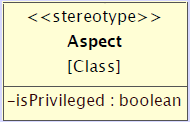
\includegraphics[width=100px]{img/p21_meta_class.png}
	\caption{Exemplo de estereótipo estendendo uma meta-classe em um diagrama de Perfil UML.}\label{fig:p21_meta_class}
\end{figure}

O Perfil UML completo proposto por Evermann pode ser visualizado na figura \ref{fig:p21_aspectj_profile}. Como todas as construções são definidas em
linguagem de meta-modelo, pode-se realizar a geração de código em AspectJ. É de responsabilidade do desenvolvedor elaborar uma modelagem que esteja de acordo 
com as construções da linguagem alvo para geração do código. 

\begin{landscape}
\begin{figure}
	\centering
	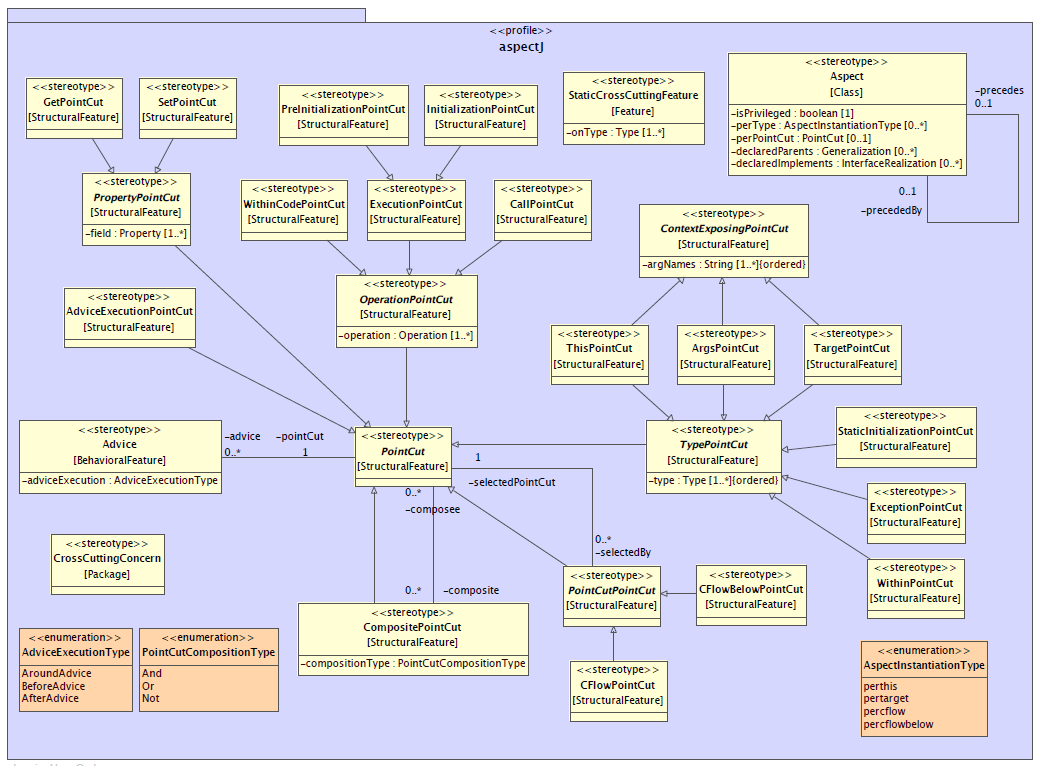
\includegraphics[width=650px]{img/p21_aspectj_profile.png}
	\caption{Perfil UML para modelagem de aspectos \cite{Evermann:2007:MSP:1229375.1229379}}\label{fig:p21_aspectj_profile}
\end{figure}
\end{landscape}

Para exemplificar o uso deste Perfil UML em uma modelagem, Evermann implementou o padrão de projeto Observador \cite{Gamma:1995:DPE:186897} em um
sistema para desenho de interface gráfica. O diagrama de classes do interesse núcleo pode ser visualizado na figura \ref{fig:p21_base_model}. 

\begin{figure}
	\centering
	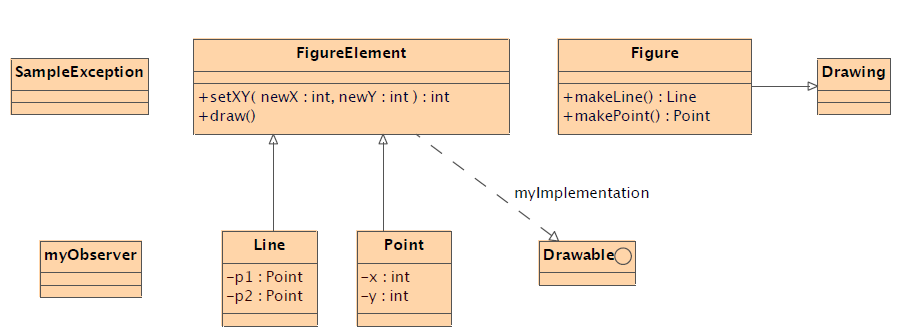
\includegraphics[width=400px]{img/p21_base_model.png}
	\caption{Interesse núcleo para desenho de interface gráfica}\label{fig:p21_base_model}
\end{figure}

\begin{figure}
	\centering
	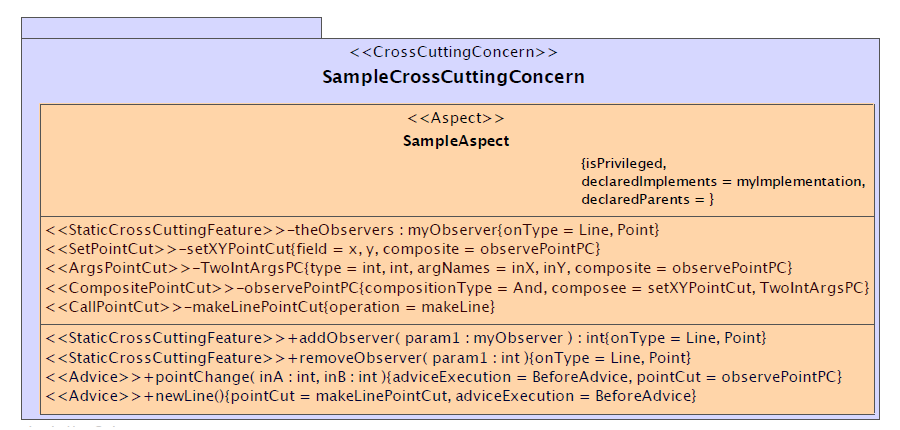
\includegraphics[width=400px]{img/p21_extension_model.png}
	\caption{Interesse entrecortante para implementação do padrão de projeto Observador}\label{fig:p21_extension_model}
\end{figure}

O interesse entrecortante é o padrão de projeto Observador e a sua modelagem  pode ser visualizada na figura \ref{fig:p21_extension_model}. 
O modelo do interesse entrecortante contém um aspecto que especifica quatro pontos de corte, três introduções e dois avisos. O ponto de corte
\textit{setXYPointCut} captura modificações nos atributos x e y da classe \textit{Point}. O ponto de corte  \textit{twoIntArgsPC} captura chamadas e
execuções com dois argumentos do tipo inteiro. O ponto de corte \textit{observePointPC} compõe os dois pontos de cortes anteriores com o operador \textit{And},
capturando modificações nos atributos x e y da classe \textit{Point} com dois argumentos do tipo inteiro. Finalmente, define-se o ponto de corte 
\textit{makeLinePointCut} que captura chamadas ao método \textit{makeLine()}. As introduções adicionadas são os métodos \textit{addObserver()} e
\textit{removeObserver()} e o atributo \textit{theObservers} nas classes \textit{Line} e \textit{Point}. Estes membros permitem adicionar, remover e
armazenar os observadores. Para introduzir os novos comportamentos, especifica-se o aviso \textit{pointChange} que é executado antes do ponto de
corte \textit{observePointPC} e o aviso \textit{newLine} que é executado antes do ponto de corte \textit{makeLinePointCut}. A composição do interesse
entrecortante no interesse núcleo pode ser visualizada na figura \ref{fig:p21_code}. A composição é realizada em nível de código.

\begin{figure}
	\centering
	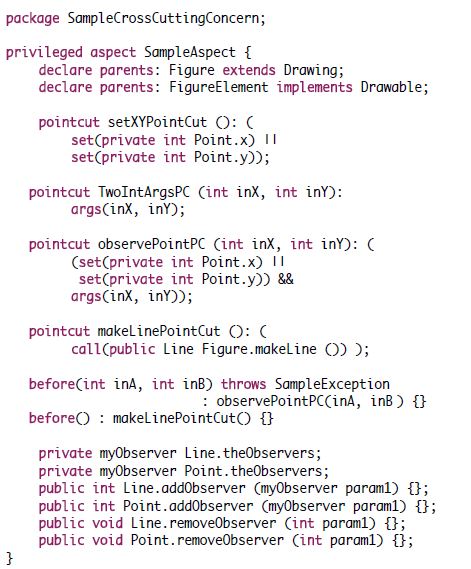
\includegraphics[width=300px]{img/p21_code.png}
	\caption{Composição do padrão observador no sistema de interface gráfica (em nível de código)}\label{fig:p21_code}
\end{figure}

A principal contribuição deste trabalho é a especificação do meta-modelo apenas em termos da UML, sem a necessidade de descrições textuais e de
ferramentas adicionais para interpretação ou geração de código a partir do modelo. Além disso, o meta-modelo pode ser utilizado como um perfil UML em
ferramentas que suportem a importação de perfis. Com a representação de elementos apenas em termos de meta-modelo, perde-se a possibilidade de
representar padrões para captura de pontos de junção: os \textit{wildcards}. A especificação por padrões é uma importante
funcionalidade da programação por aspectos, pois simplifica a forma de capturar pontos de junção, sem a necessidade de explicitar cada elemento que
será capturado. Assim, é importante que a extensão à UML permita representar essas características de uma maneira simples e praticável, para que seja
possível expressar todas as características da POA na modelagem.

O trabalho de \cite{Evermann:2007:MSP:1229375.1229379} permite representar a estrutura de um programa orientado a aspectos através das meta-classes
\textit{CrossCutingConcern}, \textit{Aspect}, \textit{PointCut} e \textit{StaticCrossCutingFeatures}. É importante observar que apenas a parte
estrutural é especificada por esta proposta. Em relação às características comportamentais, como a meta-classe \textit{Advice} estende a meta-classe
\textit{BehavioralFeature}, é possível representá-las com colaborações e diagramas de máquinas de estados, mas o trabalho não demonstra como realizar
a modelagem de colaborações e nem permite a composição automatizada entre modelos que representam aspectos dinâmicos do sistema. Assim, conclui-se que
o foco do trabalho é a representação da estrutura de um sistema orientado a aspectos. A parte dinâmica deve ser implementada manualmente no código
gerado, que é uma limitação da abordagem, pois o desenvolvedor não pode especificar e visualizar a dinâmica de aspectos nos modelos que
representam o sistema.

\section{Modelos de Aspectos Reusáveis (RAM) Proposto por Kienzle}

Uma modelagem por múltiplos pontos de vista é proposta por Kienzle \cite{Kienzle:2009:AMM:1509239.1509252} \cite{Kienzle2010}. Propõe-se RAM
(\textit{Reusable Aspects Models}), uma abordagem para especificar aspectos com dois diagramas dinâmicos (diagrama de máquina de estados e de sequência) e um diagrama estrutural (diagrama de
classes). O objetivo deste trabalho é a melhora da escalabilidade de um sistema, mantendo a consistência entre as diferentes visões de um interesse
entrecortante. RAM define modelos base para representar interesses núcleo e de aspectos para representar interesses entrecortantes.

Duas ferramentas são utilizadas para a composição dos modelos. \textit{Kompose} \cite{kompose:07} é utilizado para composição da parte estrutural
(diagramas de classe). Para composição, os elementos do modelo devem ser instâncias da mesma classe do meta-modelo. A composição é realizada
comparando a assinatura de tipo dos elementos. Cada elemento do modelo deve possuir uma assinatura de tipo que o representa unicamente na modelagem.
Dois elementos que tiverem a mesma assinatura podem ser compostos. A composição de diagramas de sequência e de estado é realizada utilizando uma outra
ferramenta denominada GeKo \cite{geko:08}. Com essa ferramenta, para inserção de um novo comportamento em um modelo núcleo deve-se definir um modelo 
entrecortante (aspecto). Esse modelo de aspecto é composto por um diagrama refinando o ponto de corte e outro diagrama refinando o aviso. A composição
acontece em duas fases: primeiramente são detectados os elementos do modelo núcleo que são impactados pelo ponto de corte do modelo do aspecto. Com os 
elementos capturados executa-se um mecanismo de composição que gera o modelo composto com o comportamento (aviso)
do modelo do aspecto inserido no modelo núcleo (antes, durante ou depois). Essas duas ferramentas permitem representar aspectos e a composição entre
um modelo núcleo e um modelo de aspecto.

Um interesse em RAM é modelado através de um pacote UML. Este pacote contém três visões: estrutural, de estado e de mensagens e é denominado modelo de
um aspecto, podendo ser reusado em diferentes aplicações. A visão estrutural é composta por diagrama de classes. Nesta visão, as classes não precisam
ser completamente especificadas, pois só precisam expressar o que é relevante para o interesse em questão. A visão de estado descreve o protocolo de
uso de uma classe. Para classes completas, utiliza-se o diagrama de máquina de estados da UML. Classes incompletas são modeladas com um diagrama de
máquina de estados para aspectos, composto por uma parte representando o ponto de corte e outra representando o aviso. O ponto de corte determina
quais estados devem existir para o aviso ser executado. A visão de troca de mensagens utiliza o diagrama de sequência, onde cada método público das
classes modeladas deve ser representando. Aqui também pode-se especificar o comportamento de aspectos através de dois diagramas de sequência:
um para o ponto de corte e outro para o aviso. O ponto de corte determina a sequência de mensagens que deve ocorrer pra ativar o aviso. O aviso
descreve a sequência de mensagens que substituem o ponto de corte em uma execução. Nas três visões, alguns elementos podem estar incompletos, o que
significa que eles não são especificados no modelo de aspecto e deverão ser especificados por algum outro modelo na composição de modelos. Esses
elementos são denominados \textbf{parâmetros de instanciação mandatória}, identificados pelo prefixo | e modelados como parâmetros de
\textit{template} UML.

RAM permite estabelecer dependências entre aspectos, com o objetivo de possibilitar o reuso de modelos. Se um aspecto A depende de um aspecto B, A
deve instanciar todos os parâmetros de instanciação mandatória de B através de \textbf{diretivas de instancialização}. Por exemplo, para uma
classe incompleta em B, A deve especificar uma classe que possa completá-la com os métodos e atributos faltantes. Esta regra vale também para as visões de
estado e de mensagens. Além disso, A pode definir \textbf{diretivas de ligação} que mapeiam entidades incompletas de A em entidades completas de B.
Nesse caso, as entidades incompletas de A não podem ser parâmetros de instanciação mandatória. É importante observar que diretivas de ligação e
parâmetros de instanciação mandatória podem ser definidos com \textit{wildcards}, permitindo a captura de padrões, uma funcionalidade
importante da programação por aspectos.

A proposta de Kienzle também realiza a verificação de consistências entre as diferentes visões e modelos de aspectos. São realizadas verificações em
diferentes níveis:

\begin{itemize}
  \item \textbf{No modelo de aspecto}: Pode-se verificar se existe um diagrama de máquina de estados para cada classe na visão estrutural.
  \item \textbf{Entre modelos de aspectos}: Pode-se verificar que um aspecto A que depende de B deve inicializar todos os parâmetros de instanciação
  mandatórios de B.
  \item \textbf{No modelo final}: Pode-se comparar a sequência de mensagens na visão de mensagens com o diagrama de máquina de estados. As mensagens
  devem obedecer o protocolo do diagrama de máquina de estados.
\end{itemize}

Um estudo de caso foi realizado para avaliar a modelagem por múltiplos pontos de vista. No estudo adiciona-se a funcionalidade de garantia de
atomicidade em um modelo de transações. O modelo de transações bancárias (modelo núcleo) pode ser visualizado na figura \ref{fig:p87_base_model}. Para
garantir a atomicidade de transações utiliza-se o aspecto \textit{Recovering} que tem dependência com nove aspectos. Este aspecto pode ser visualizado 
na figura \ref{fig:p87_recovering_aspect.png}. Uma das dependências indiretas é o aspecto \textit{Checkpointable} (\textit{Recovering} depende de
\textit{Checkpointing} que depende de \textit{Checkpointable}). Este aspecto permite estabelecer pontos de verificação de um objeto, armazenando o seu estado e permitindo a restauração do mesmo. O aspecto \textit{Checkpointable} depende 
de um outro aspecto denominado \textit{Copyable} e ele deve instancializar os elementos incompletos de \textit{Copyable}. Um exemplo de
instancialização pode ser visualizado na visão de mensagens do aspecto \textit{Checkpointable}. A diretiva de instancialização \textit{clone.ICaller-ICheckpointable} 
indica que o objeto \textit{ICaller} da visão de mensagens do método \textit{clone} em \textit{Copyable} está sendo instancializado com o objeto
\textit{ICheckpointable} de \textit{Checkpointable}. O aspecto \textit{Recovering} também contém diretivas de instancialização para os elementos 
incompletos dos aspectos os quais depende.

\begin{figure}[!hb]
	\centering
	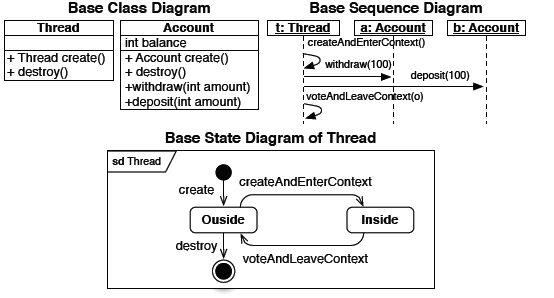
\includegraphics[width=375px]{img/p87_base_model.png}
	\caption{Modelo núcleo para transações}\label{fig:p87_base_model}
\end{figure}

Com o aspecto para garantia de atomicidade definido, deve-se realizar a composição com o modelo núcleo. O modelo final após a composição pode ser
visualizado nas figuras \ref{fig:p87_class_final_model} (visão estrutural), \ref{fig:p87_state_final_model} (visão de estados) e \ref{fig:p87_sequence_final_model} (visão de mensagens). 
Observa-se a presença de alguns elementos referentes ao aspecto \textit{Checkpointable} no modelo final como a classe \textit{Stack} e a inserção dos métodos \textit{establish(),
restore()} e \textit{discard()} na visão de mensagens. Na visão de troca de mensagens, as mensagens referentes ao aspecto \textit{Checkpointable}
também estão destacadas. Nesta visão, as mensagens de cada aspecto dependente estão destacadas. Assim, o modelo final contém uma parte de cada
aspecto, compostas com o modelo núcleo, resultando em um modelo que representa o comportamento desejado para garantia de atomicidade de transações.

\begin{landscape}
\begin{figure}
	\centering
	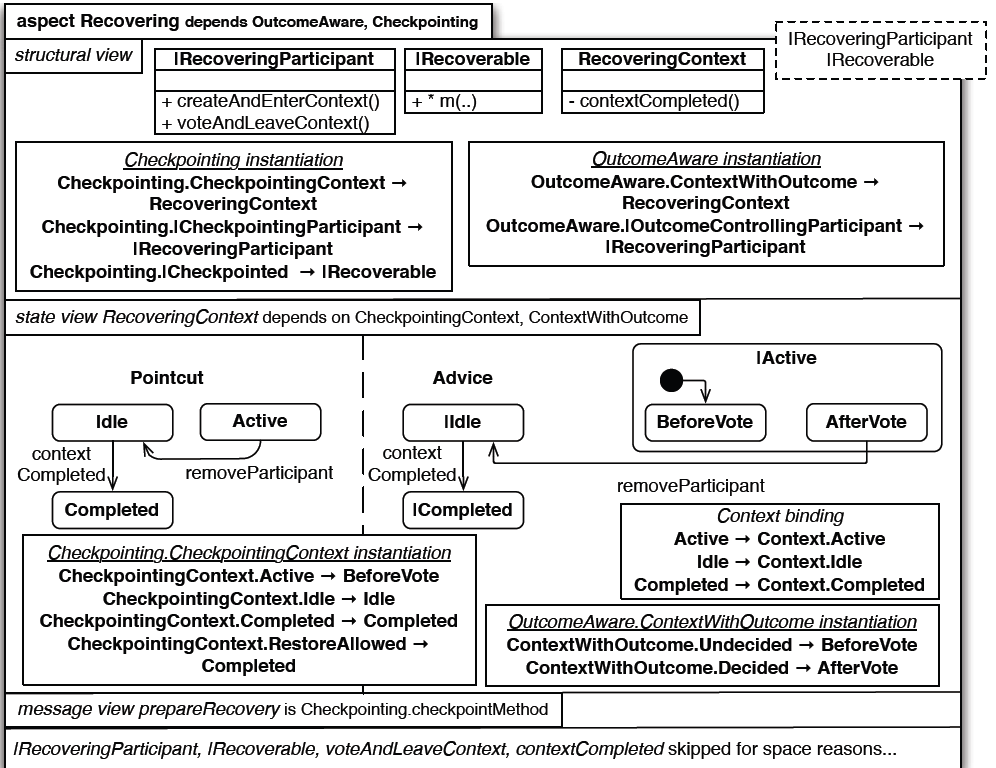
\includegraphics[width=450px]{img/p87_recovering_aspect.png}
	\caption{Aspecto para recuperação de dados (garantia de atomicidade)}\label{fig:p87_recovering_aspect.png}
\end{figure}
\end{landscape}

\begin{landscape}
\begin{figure}
	\centering
	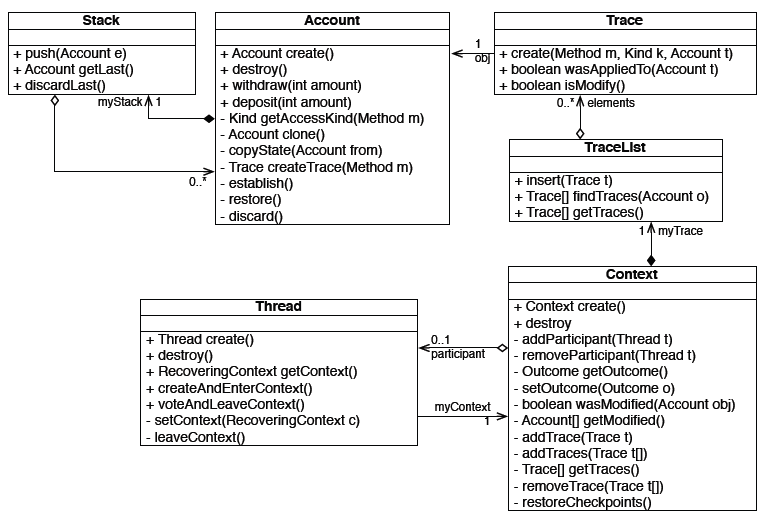
\includegraphics[width=500px]{img/p87_class_final_model.png}
	\caption{Visão estrutural do modelo final para garantia de atomicidade de transações}\label{fig:p87_class_final_model}
\end{figure}
\end{landscape}

\begin{landscape}
\begin{figure}
	\centering
	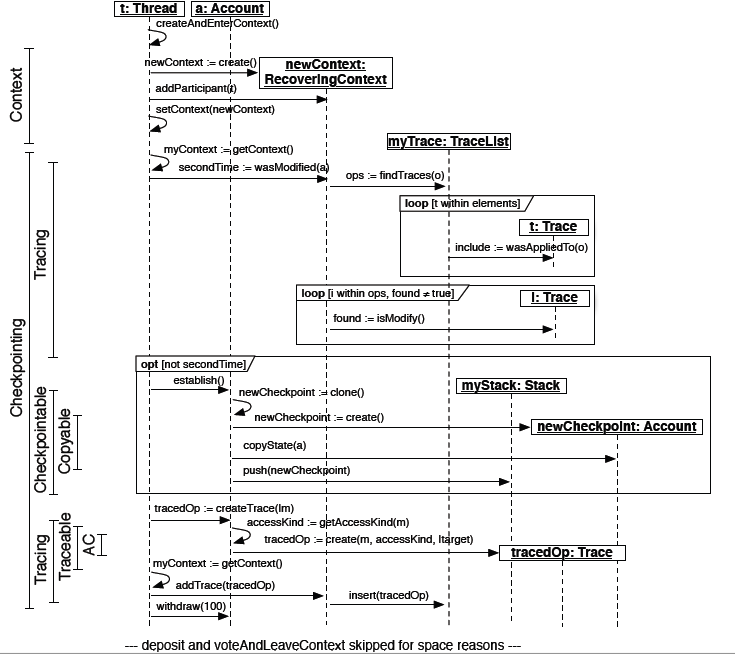
\includegraphics[width=500px]{img/p87_sequence_final_model.png}
	\caption{Visão de mensagens do modelo final para garantia de atomicidade de transações}\label{fig:p87_sequence_final_model}
\end{figure}
\end{landscape}

\begin{landscape}
\begin{figure}
	\centering
	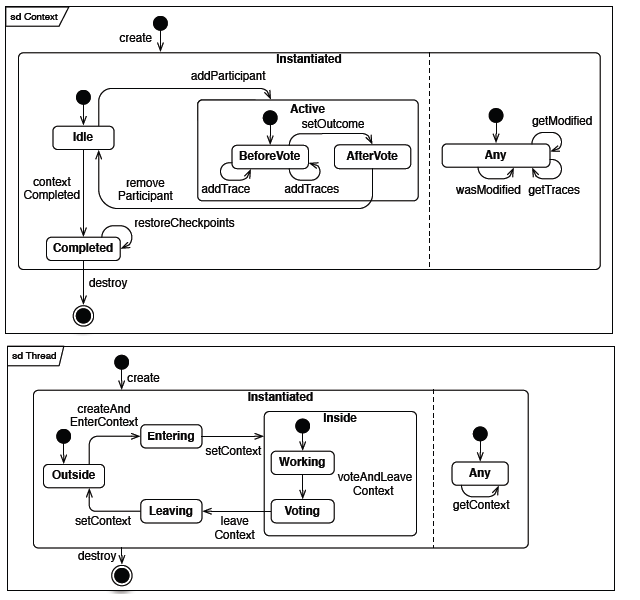
\includegraphics[width=400px]{img/p87_state_final_model.png}
	\caption{Visão de estados do modelo final para garantia de atomicidade de transações}\label{fig:p87_state_final_model}
\end{figure}
\end{landscape}

A abordagem RAM permite representar a estrutura de ums sistema através da visão estrutural e a dinâmica do sistema através das visões de estado
e de troca de mensagens. A maior contribuição deste trabalho é o foco na representação das caracaterísticas dinâmicas de um sistema, utilizando
diagramas de máquinas de estado para representar o protocolo de um aspecto e diagramas de sequência para representar as possíveis interações entre
objetos. A especificação de pontos de corte com padrões (\textit{wildcards}) também é suportada pela ferramenta, permitindo assim o uso de uma 
importante funcionalidade da programação orientada a aspectos. Outra característica importante de RAM é a garantia de consistência entre as
diferentes visões e a orientação ao reuso de aspectos através da definição de dependências. 

Uma limitação da proposta é que nem todos os diagramas podem ser elaborados apenas estendendo a UML, pois a abordagem realiza modificações no
meta-modelo da UML, introduzindo novos conceitos que não estão presentes na versão padrão da OMG. Exemplos são as diretivas de instancialização e as diretivas de ligação. 
A complexidade do modelo composto também pode ser considerada uma limitação da abordagem, pois o modelo gerado é extenso, o que dificulta a
compreensão, já que existem muitas dependências indiretas entre aspectos e muitos elementos sintáticos na modelagem. Segundo \cite{seventwo:11},
quando uma pessoa entra em contato com novas informações, o limite de sua memória de trabalho é entre três ou quatro elementos de informação. A
modelagem proposta por Kienzle é difícil de ser compreendida, pois o modelo final (composto) contém muitos
elementos de informação. No exemplo de composição de aspectos, o modelo final contém elementos que vieram de nove diferentes aspectos. Além disso, contém elementos
que não são padrões na modelagem de sistemas com UML, como as diretivas de instancialização e de ligação. Para facilitar a compreensão do
comportamento dinâmico de uma modelagem, este trabalho poderia disponibilizar um visualizador de aspectos, que permitisse habilitar e desabilitar
modelos de aspectos dinamicamente em um modelo núcleo, diferenciando os aspectos no modelo final.

\section{Modelagem de Aspectos com Atividades Proposto por Cui}

O trabalho de Cui, \cite{Cui:2009:MIA:1529282.1529377} modela a dinâmica de um sistema com diagramas de atividades da segunda versão da UML. Os
interesses núcleo são modelados com a versão padrão da UML. No caso dos interesses entrecortantes, é proposta uma extensão ao diagrama de atividades com
estereótipos e valores rotulados. Um interesse entrecortante é representado por dois modelos: um para o ponto de corte e outro para o aviso.
Adiciona-se o estereótipo \textit{Pointcut} para indicar que um diagrama de atividades representa um \textbf{modelo de ponto de corte}. O estereótipo
\textit{Pointcut} tem um valor rotulado denominado \textit{advice} que aponta para o nome do modelo de aviso associado a este ponto de corte. Para
representar os pontos de execução de um programa que serão capturados adiciona-se o estereótipo \textit{Joinpoint}. Esta abordagem permite a seleção
de pontos de junção com o uso de \textit{wildcards}. Um elemento no modelo de ponto de corte estereotipado com \textit{Argument} define os argumentos
que serão passados para o modelo de aviso. O estereótipo \textit{Argument} tem um valor rotulado denominado \textit{parameter} que define o nome dos
parâmetros que serão preenchidos no modelo de aviso. O estereótipo \textit{Advice} é adicionado para especificar que um diagrama de atividades
representa um \textbf{modelo de aviso}. O valor rotulado \textit{type} está associado com este estereótipo indicando o tipo de aviso: antes ou depois.
O estereótipo \textit{Parameter} é adicionado para representar os parâmetros que são aceitos pelo modelo de aviso. Estes parâmetros são utilizados
para possibilitar o reuso de avisos, apenas modificando os parâmetros passados na inicialização. Finalmente, adicionam-se dois estereótipos
\textit{Entry} e \textit{Exit} para especificar o início e o fim de uma execução de um modelo de aviso.
 
\begin{figure}
	\centering
	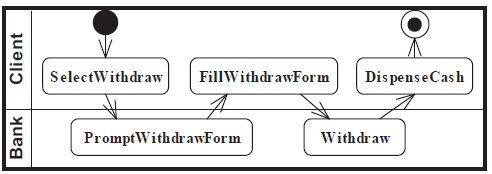
\includegraphics[width=300px]{img/withdraw_base.png}
	\caption{Modelo núcleo para realizar a transação de saque}\label{fig:withdraw_base}
\end{figure}

 A figura \ref{fig:withdraw_base} mostra o modelo núcleo de um caso de uso para realizar a transação bancária de saque. Este modelo é estendido
 utilizando a abordagem proposta por Cui, com a definição de dois pontos de corte e dois avisos. Os modelos do primeiro ponto de corte e do
 primeiro aviso podem ser visualizados na figura \ref{fig:withdraw_1}. O ponto de corte \textit{Pointcut1} seleciona os elementos no modelo núcleo
 aonde o aviso de autorização deve ser aplicado. O aviso \textit{Advice1} representa o comportamento de autorização. A figura \ref{fig:withdraw_2}
 mostra o ponto de corte \textit{Pointcut2} que pretende capturar os elementos no modelo núcleo aonde o aviso de envio de e-mail será
 aplicado. O aviso \textit{Advice2} representa o comportamento de enviar um e-mail. Observa-se uma diferença no comportamento dos dois avisos: a
 autorização é realizada antes (aviso do tipo \textit{before}) da execução dos pontos de junção selecionados pelo primeiro ponto de corte. No entanto,
 o envio de e-mail é realizado depois (aviso do tipo \textit{after}) dos pontos de junção selecionados pelo segundo ponto de corte, e, o envio de
 e-mail é realizado paralelamente ao comportamento dos pontos de junção. 

\begin{figure}
	\centering
	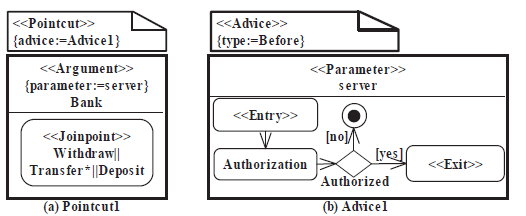
\includegraphics[width=300px]{img/withdraw_1.png}
	\caption{Ponto de corte e aviso para capturar pontos
	de junção que necessitam de autorização antes de
	serem executados}\label{fig:withdraw_1}
\end{figure}

Após a definição do modelo núcleo e dos modelos para os interesses entrecortantes, deve-se realizar a composição entre os modelos. Esta composição
consiste em três passos:

\begin{itemize}
  \item \textbf{Captura}: Encontrar os pontos de junção no modelo núcleo.
  \item \textbf{Inicialização}: Inicializar os modelos de aspectos com os parâmetros obtidos do modelo núcleo.
  \item \textbf{Composição}: Realizar a composição entre os modelos de aspectos e o modelo núcleo.
\end{itemize}

Após a composição, obtém-se o modelo final com os interesses entrecortantes introduzidos. O modelo final pode ser visualizado na figura
\ref{fig:withdraw_final}.

\begin{figure}[!t]
	\centering
	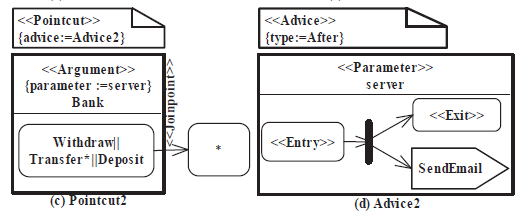
\includegraphics[width=300px]{img/withdraw_2.png}
	\caption{Ponto de corte para capturar pontos de junção onde é necessário
	enviar um e-mail após a execução dos mesmos}\label{fig:withdraw_2}
\end{figure}

A proposta de Cui é uma extensão à segunda versão da UML, estendendo apenas o diagrama de atividades com a adição de novos estereótipos e valores
rotulados para representar interesses entrecortantes. A extensão segue o padrão do meta-modelo definido pela OMG para a segunda versão da UML e 
pode ser utilizada em qualquer ferramenta que suporte a definição de perfis. É possível realizar a composição entre modelos de interesses núcleo e
modelos de interesses entrecortantes e a mesma é realizada em nível de modelo.

\begin{figure}
	\centering
	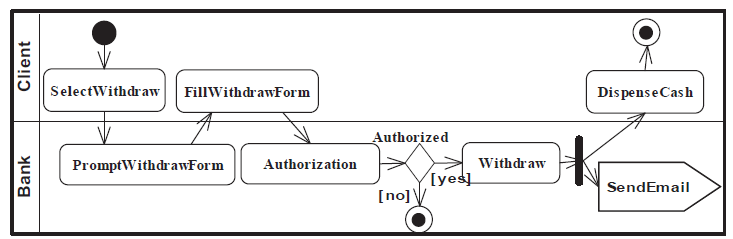
\includegraphics[width=400px]{img/withdraw_final.png}
	\caption{Modelo composto para transação bancária de
	saque com autorização e envio de e-mail}\label{fig:withdraw_final}
\end{figure}

Em relação a POA, a abordagem não permite representar as principais características do paradigma. Não é possível adicionar introduções a classes e
interfaces nos modelos de interesses núcleo. Também não é possível representar todos os tipos de ponto de junção e nem adicionar avisos do tipo \textit{around}, que permite
substituir a execução de um ponto de junção ou modificar o comportamento de execução do mesmo. Em relação as visões representadas pela modelagem, a
parte estrutural não pode ser representada apenas com diagrama de atividades e a abordagem não utiliza nenhum diagrama estrutural para representar o
sistema. Assim, esta proposta representa apenas a parte dinâmica de um sistema orientado a aspectos. A principal contribuição desta proposta é uma
extensão leve e simples aos diagramas de atividades da UML para representação da dinâmica de aspectos em alto nível de abstração.

\section{Modelagem de Aspectos com Casos de Uso Proposto por Jacobson}

O trabalho de Jacobson \cite{Jacobson:2004:ASD:1062430} utiliza casos de uso para representação de interesses entrecortantes. São identificados dois
tipos de caso de uso:

\begin{itemize}
  \item \textit{Peer Use Cases}: São casos de uso que não tem relacionamentos com outros casos de uso, mas sua implementação impacta mais de uma
  classe. São os interesses núcleo de um sistema.
  \item \textit{Extension Use Cases}: São casos de uso que estendem o comportamento de um caso de uso base. Tem relacionamentos com outros casos de
  uso e sua implementação pode impactar mais de uma classe. São os interesses entrecortantes de um sistema.
\end{itemize}

Propõe-se uma construção denominada \textbf{fatia de caso de uso} (\textit{use-case slice}) que deve modelar apenas as especificidades de um 
caso de uso. Para tal adiciona-se o estereótipo \textit{use-case slice} ao meta-modelo da UML. Uma fatia de caso de uso contém: definições de novas
classes necessárias para realizar o caso de uso, extensões a classes existentes (apenas a extensão será representada na fatia do caso de uso) e
colaborações para representar a realização do caso de uso. O gráfico da figura \ref{fig:jacobson_slices} mostra o impacto dos casos de uso nas classes
de um sistema de gerenciamento de hotel. Observa-se que os casos de uso \textit{Reserve Room}, \textit{Check In Customer} e \textit{Check Out
Customer} modificam a mesma classe \textit{Room}. Cada fatia de caso de uso define uma parte desta classe. A classe completa é obtida realizando a
composição das fatias de caso de uso. A classe \textit{StaffScreen} é modificada pelos casos de uso \textit{CheckOutCustomer} e
\textit{CheckInCustomer}. Já a classe \textit{Reservation} é modificada pelos casos de uso \textit{ReserveRoom} e \textit{CheckInCustomer}. As outras
classes são modificadas por apenas um caso de uso.

\begin{figure}
	\centering
	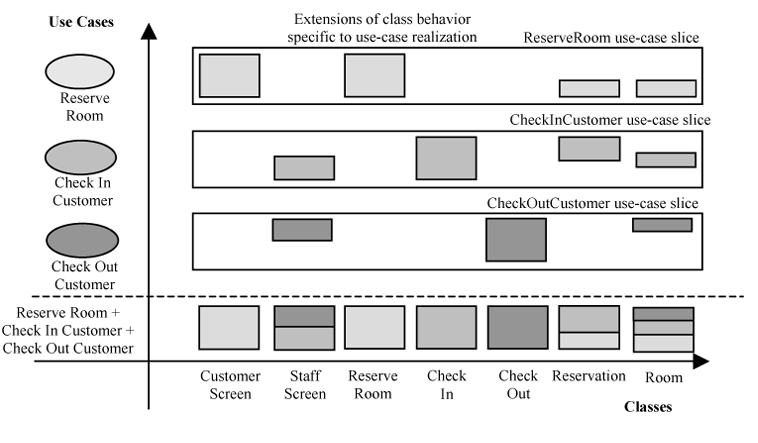
\includegraphics[width=400px]{img/jacobson_slices.png}
	\caption{Fatias de casos de uso em um sistema de
	gerenciamento de hotel}\label{fig:jacobson_slices}
\end{figure}

A figura \ref{fig:jacobson_reserve_room_slice} mostra a fatia do caso de uso \textit{Reserve Room}. As classes pertencentes a este interesse
estão dentro de um pacote estereotipado como \textit{use case slice}. Observa-se nesta figura o aspecto \textit{ReserveRoom} marcado com o estereótipo
\textit{aspect}. Dentro deste aspecto definem-se extensões à três classes do modelo: \textit{CustomerMainForm}, \textit{Reservation} e \textit{Room}.
A representação de extensões à classes é equivalente às introduções da linguagem AspectJ. Esta fatia de caso de uso define também
duas novas classes: \textit{ReserveRoomForm} e \textit{ReserveRoomHandler}. Este caso de uso é do tipo \textit{peer} (\textit{Peer Use Case}), pois
ele não estende nenhum caso de uso, apenas define novas classes e introduz métodos em classes já existentes.

\begin{figure}
	\centering
	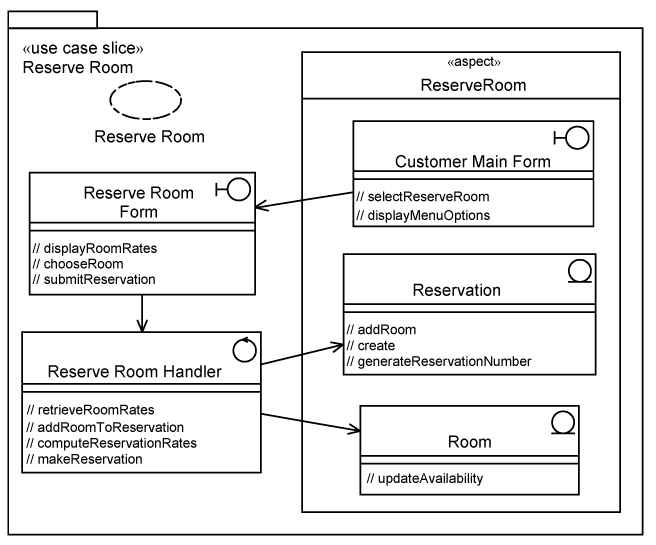
\includegraphics[width=450px]{img/jacobson_reserve_room_slice.png}
	\caption{Fatia de caso de uso para o
	caso de uso \textit{Reserve Room}}\label{fig:jacobson_reserve_room_slice}
\end{figure}

Os casos de uso de extensão (\textit{Extension Use Cases}) estendem o comportamento de um caso de uso base. A figura
\ref{fig:jacobson_use_case_extension} mostra o caso de uso \textit{Handle Waiting List} que estende o caso de uso \textit{Reserve Room}. Um caso de
uso base define um conjunto de \textbf{pontos de extensão} representando os pontos que podem ser estendidos por outros casos de uso. Um caso de uso de
extensão define \textbf{pontos de corte de extensão} para representar quais pontos de extensão do caso de uso base serão estendidos. 

\begin{figure}
	\centering
	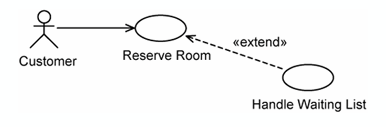
\includegraphics[width=300px]{img/jacobson_use_case_extension.png}
	\caption{Caso de uso de extensão
	\textit{Handle Waiting List}}\label{fig:jacobson_use_case_extension}
\end{figure}

A fatia de caso de uso da figura \ref{fig:jacobson_handle_waiting_list_slice} mostra a modelagem do caso de uso de extensão \textit{Handle Waiting
List}, que adiciona o cliente em uma lista de espera se não for possível reservar um quarto. Para tal, o caso de uso de extensão define o ponto de
corte \textit{updatingRoomAvailability} para capturar as chamadas ao método \textit{UpdateAvailability()} da classe \textit{Room}. Dentro do aspecto
define-se uma extensão à classe \textit{ReserveRoomHandler}, adicionando o método \textit{makeReservation()}. Este método será executado depois
do ponto de corte \textit{updatingRoomAvailability} quando forem lançadas as exceções \textit{NoRoomAvailable} ou \textit{QueueForRooms}. Além disso,
são introduzidos dois novos métodos à classe \textit{Reservation} relativos a reserva de quartos. Esta fatia de caso de uso cria duas novas classes:
\textit{WaitingListHandler} e \textit{WaitingList}.

\begin{figure}
	\centering
	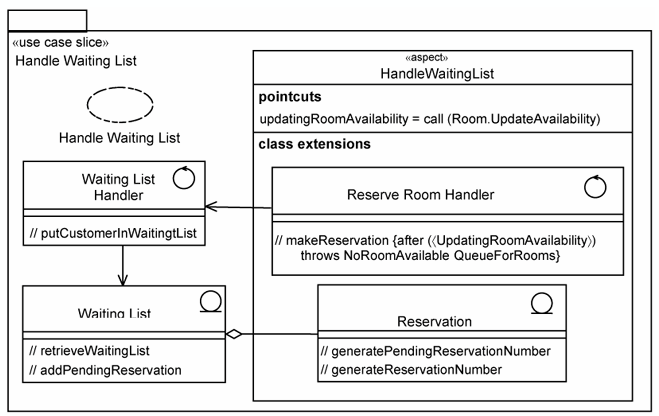
\includegraphics[width=450px]{img/jacobson_handle_waiting_list_slice.png}
	\caption{Fatia do caso de uso de extensão \textit{Handle Waiting List}}\label{fig:jacobson_handle_waiting_list_slice}
\end{figure}

A proposta de Jacobson propõe a definição de \textbf{modelos de caso de uso} para agrupar as fatias de caso de uso em
diferentes níveis de abstração. Define-se o estereótipo \textit{use-case module} no meta-modelo. São propostos quatro níveis de modelo: caso de uso,
análise, projeto e implementação. A fatia de caso de uso será refinada de acordo com o nível de abstração. Esta proposta consegue obter o rastreamento
completo do requisito para o código que o implementa, passando pelos modelos de caso de uso, análise e projeto, como pode ser visualizado 
na figura \ref{fig:jacobson_use_case_modules}. 

\begin{figure}
	\centering
	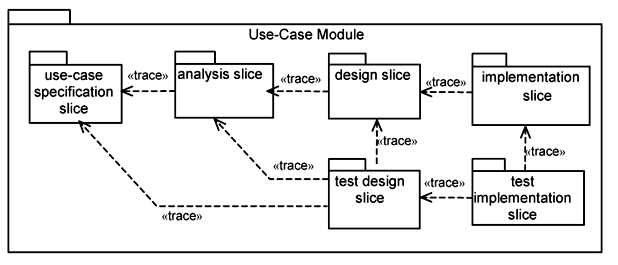
\includegraphics[width=450px]{img/jacobson_use_case_modules.png}
	\caption{Rastreamento completo de um requisito por todos modelos}\label{fig:jacobson_use_case_modules}
\end{figure}

Após a definição das fatias de caso de uso em diferentes níveis de abstração, deve-se compor os modelos de caso de uso para se obter um sistema
completo com o comportamento de cada caso de uso inserido nas respectivas classes. A figura \ref{fig:jacobson_use_case_merge} mostra a composição de
três modelos de casos de uso (cada modelo representado como um pacote UML) para gerar uma construção válida do sistema. Para tal utiliza-se o
estereótipo \textit{merge} que representa dependência entre pacotes.

\begin{figure}
	\centering
	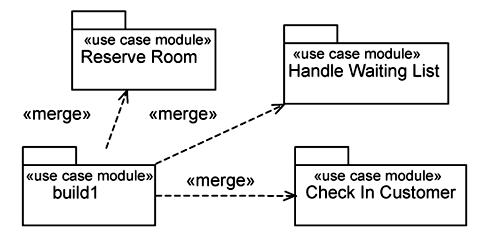
\includegraphics[width=350px]{img/jacobson_use_case_merge.png}
	\caption{Composição entre modelos de caso de uso}\label{fig:jacobson_use_case_merge}
\end{figure}

A proposta de Jacobson permite representar \textit{wildcards} na definição de pontos de corte dentro de uma fatia de caso de uso. Uma contribuição
importante deste trabalho é a possibilidade de obter o rastreamento completo de um requisito até o código que o implementa. Segundo \cite{wimmer:2011:SUA:1978802.1978807}, 
o mapeamento de requisitos entre as diferentes fases do desenvolvimento é importante na modelagem de sistemas orientados a aspectos, como para
sistemas desenvolvidos em outros paradigmas como programação orientada a objetos. Em relação as diferentes visões representadas por uma modelagem, os
modelos propostos por este trabalho permitem representar a estrutura de um sistema com fatias de caso de uso e diagramas de classes. A dinâmica do sistema 
é representada através de colaborações que são associadas às fatias de caso de uso. Colaborações podem ser utilizadas para descrever a dinâmica de
casos de uso e avisos. Outro ponto importante a ser destacado é a representatividade do exemplo utilizado para realizar uma modelagem com a proposta. 
O sistema de gerenciamento de hotel é complexo e contém interesses entrecortantes de diversos tipos, possibilitando a representação de boa parte das
características inerentes a programas orientados a aspectos.

Em relação as limitações do trabalho de Jacobson, a principal delas é a forma de extensão à UML, com a definição de um meta-modelo, que não pode ser utilizado 
em qualquer ferramenta CASE. Este meta-modelo tem construções específicas, como fatias de caso de uso, que não são suportadas por ferramentas CASE que
obedecem os padrões da segunda versão da UML. Destaca-se também a falta de ferramental para composição dos modelos, o que é
importante para que seja possível visualizar o impacto dos interesses entrecortantes nos interesses núcleo do sistema. Não é possível realizar a
composição de pontos de corte entre modelos e visualizar a conexão entre os pontos de corte e os avisos nos modelos. Assim, a abordagem proposta por
Jacobson não permite visualizar completamente o efeito dos aspectos nos modelos núcleo do sistema. A geração automática de modelos também diminui o
tempo necessário para realização de uma modelagem, diminuindo o tempo de entrega ao cliente. Nesta proposta, a composição entre interesses núcleos e
interesses entrecortantes deve ser realizada manualmente, com o uso de diagramas de sequência, o que demanda um esforço adicional de modelagem.

\section{Motorola WEAVR Proposto por Cottenier}

Uma das unidades de negócio mais importantes da Motorola também está focada no desenvolvimento de soluções para modelagem de programas orientados a
aspectos. O trabalho de Cottenier \cite{Cottenier06themotorola} \cite{Cottenier:2007:SAC:1229375.1229377} foi desenvolvido na unidade de negócios empresariais e de redes da
Motorola. O projeto é denominado de \textbf{Motorola WEAVR} e é focado na especificação de sistemas de telecomunicações, que são sistemas reativos
discretos e orientados a eventos. Um sistema reativo é um sistema que recebe uma entrada e deve emitir uma reação a este estímulo. Já um sistema discreto é um sistema cuja
interação ocorre em eventos discretos no tempo. A motivação para este trabalho foi a percepção de que existem muitas mudanças nos requisitos de 
sistemas de telecomunicação ao longo do desenvolvimento. A modularização de interesses facilita a manutenabilidade e a inserção de novos requisitos ao
longo do ciclo de vida desse tipo de sistema. 

Motorola WEAVR permite a composição de aspectos que são modelados \textbf{com diagramas de máquina de estados focadas em transições}. Este tipo de
máquina de estado é uma extensão à máquina de estados da UML focada em estados, com o objetivo de prover um maior nível de detalhe na dinâmica das
transições. Segundo Bjorkander \cite{Bjorkander:2000:GPU:619058.621607}, o diagrama de máquina de estados focado em estados da UML não dá a atenção
que as transições merecem. Estas máquinas de estado ignoram as ações que ocorrem durante uma transição. A linguagem Specification and Description Language
(SDL) \sigla{SDL}{Specification and Description Language} \cite{sdl:00} foca nas ações que acontecem durante uma transição. Esta linguagem é
amplamente utilizada para especificar sistemas orientados a eventos na área de telecomunicações. Assim, a extensão proposta foca nas ações que ocorrem
durante uma transição e estende o diagrama de máquina de estados da UML com novas construções que permitem representar as ações de uma transição. O
diagrama de máquina de estados focado em transições permite diminuir o nível de abstração de uma modelagem, aproximando-o ao código
e permitindo a geração de código em uma linguagem alvo. A modelagem de ações que ocorrem durante transições já está disponível na especificação
do diagrama de máquina de estados da segunda versão da UML através deu um perfil UML \cite{uml:05}.

Esta abordagem também utiliza diagramas de estrutura composta da segunda versã da UML para especificar as interfaces do sistema e os componentes em
termo de sinais necessários e realizados. Este tipo de diagrama raramente é modificado durante o ciclo de vida de um sistema, por isso não são
utilizados na modelagem de programas orientados a aspectos. O diagrama da figura \ref{fig:weavr_composite_structure} mostra um diagrama de estrutura
composta para representar a estrutura de um servidor de recursos. Um servidor de recursos é composto por um despachante \textit{Dispatcher} e por um
ou mais tratadores de requisições \textit{RequestHandler}. O despachante tem a responsabilidade de passar requisições externas para um dos tratadores
de requisições. Um tratador de requisições é responsável por controlar o acesso a recursos, permitindo o acesso apenas se todos os recursos
necessários estiverem disponíveis. Esse tipo de controle pode ser implementado com o protocolo \textit{Two Phase Commit} \sigla{2PC}{Two Phase
Commit}.

\begin{figure}
	\centering
	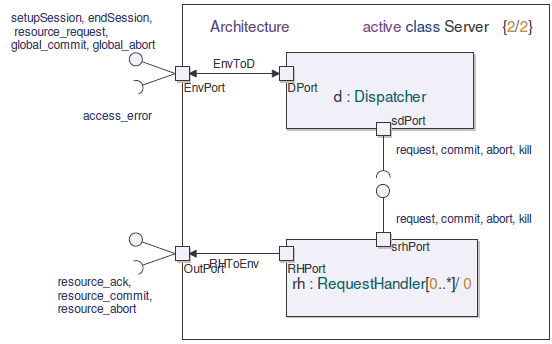
\includegraphics[width=350px]{img/weavr_composite_structure.png}
	\caption{Diagrama de Estrutura Composta
	representando um servidor de recursos}\label{fig:weavr_composite_structure}
\end{figure}

Após modelar a estrutura do sistema, deve-se modelar a dinâmica de cada um dos componentes do servidor. Para tal, utilizam-se os diagramas de
máquina de estado focados em transições. Estes diagramas são utilizados para representar o comportamento de um componente em detalhes (sem
ambiguidades). Um diagrama deste tipo destaca o fluxo de controle e as ações executadas durante as transições entre os diferentes estados. A figura
\ref{fig:weavr_state_machine_base} representa a modelagem do comportamento de um tratador de requisições.

\begin{figure}
	\centering
	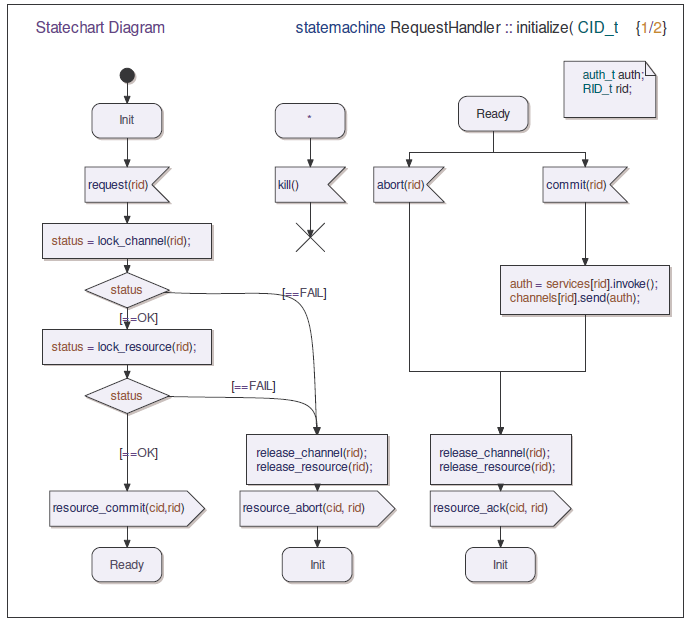
\includegraphics[width=450px]{img/weavr_state_machine_base.png}
	\caption{Diagrama de máquina de estados focado em transições
	para um tratador de requisições}\label{fig:weavr_state_machine_base}
\end{figure}

Observando o primeiro diagrama de máquina de estados, verifica-se a presença de um conjunto de ações entre os estados \textit{Init} e \textit{Ready}. 
A primeira ação \textit{request(rid)} indica o recebimento de um sinal para iniciar uma requisição. A segunda ação dentro de um retângulo tenta
adquirir o canal e armazena o resultado na variável \textit{status}. Após estas ações está presente um nodo decisão para verificar a variável
\textit{status}. Se o resultado for um \textit{OK}, significa que o canal foi adquirido com sucesso e executa-se uma nova ação para adquirir o recurso
desejado, armazenando o resultado na variável \textit{status}. Se o valor da variável \textit{status} no nodo decisão for \textit{OK}, executa-se a
ação \textit{resource\_commit(cid,rid)} que indica o envio de um sinal. Este sinal indica que o recurso foi adquirido. Finalmente, atinge-se o estado
\textit{Ready}. Se em algum momento a variável \textit{status} retornar uma falha, o canal e o recurso serão liberados, abortando a acquisição do
recurso. Todas estas ações ocorrem durante o disparo de uma transição. 

No ambiente distribuído da Motorola existem vários sistemas que utilizam o protocolo 2PC no tratamento de requisições. Cada sistema implementa uma
variação deste protocolo. A implementação do protocolo apenas com POO é possível, mas gera um código emarranhado e de difícil manutenção, pois o
código do protocolo fica misturado com o código da aplicação. A POA permite implementar de maneira modular o protocolo 2PC. Esta foi uma das
motivações para criação da ferramenta \textbf{Motorola WEAVR}. 

Esta ferramenta define um perfil UML para modelagem de aspectos. A extensão proposta por Cottenier pode ser reutilizada em outras
ferramentas de modelagem. O perfil adiciona o estereótipo \textit{Aspect} que estende o elemento \textit{Class} do meta-modelo da UML. Um aspecto pode 
conter conectores e pontos de corte. Um conector é o equivalente a um aviso na terminologia de aspectos. O estereótipo
\textit{Connector} foi criado para representar um conector. Para representar pontos de corte utiliza-se o estereótipo \textit{Pointcut}. Estes
estereótipos estendem o elemento do meta-modelo \textit{Operation}. Conectores são associados a pontos de corte através do relacionamento de
dependência \textit{Binds}. A ordem de precedência de conectores é definida pelo relacionamento de dependência \textit{Follows}. O estereótipo
\textit{Crosscuts} define o escopo de aplicação de um aspecto. Se nenhum escopo for definido, indica que o aspecto é aplicado a todo o sistema.

A figura \ref{fig:weavr_timeout} mostra a implementação de um aspecto de controle de tempo (\textit{timeout}) para o protocolo 2PC. A motivação para
implementação deste aspecto é que o tratador de requisições da figura \ref{fig:weavr_state_machine_base} tem um problema: se uma instância entrar no
estado \textit{Ready}, mas não receber nenhum sinal do tipo \textit{Commit} ou \textit{Abort}, ela nunca terminará e não poderá receber
novas requisições. Para solucionar este problema, adiciona-se um tempo máximo para que esta instância receba um sinal. Ao final deste tempo, a
instância será destruída. Este comportamento é introduzido através do aspecto \textit{2PCTimeoutAspect} que pode ser visualizado na figura
\ref{fig:weavr_timeout}. 

\begin{figure}
	\centering
	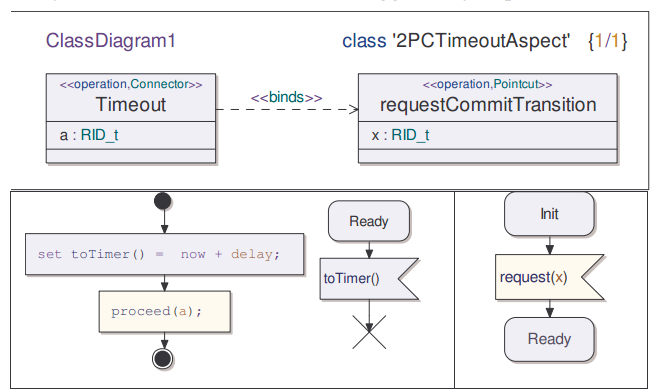
\includegraphics[width=350px]{img/weavr_timeout.png}
	\caption{Aspecto para controle de tempo ao protocolo 2PC}\label{fig:weavr_timeout}
\end{figure}

Um dos elemenos definidos neste aspecto é o ponto de corte \textit{requestCommitTransition}. A ferramenta WEAVR permite definir pontos de 
corte com o uso do diagrama de máquina de estados. Existem duas categorias de pontos de junção que que foram identificados nos diagramas de máquinas
de estado:

\begin{itemize}
  \item \textbf{Pontos de junção de ação}: Englobam as chamadas de operações, ações temporais e chamadas de construtores. 
  \item \textbf{Pontos de junção de transição}: Compreendem o conjunto de caminhos de execução dentro de uma máquina de estados.
\end{itemize}

O ponto de corte \textit{requestCommitTransition} captura pontos de junção de transição, pois captura execuções ao método \textit{request(x)} enquanto
uma instância estiver entre os estados \textit{Init} e \textit{Ready}, capturando um conjunto de caminhos de execução. Quando o ponto de corte for
disparado, executa-se o comportamento descrito no conector \textit{Timeout}. A ferramenta WEAVR representa a dinâmica de conectores através de
diagrama de máquina de estados. Este conector é refinado em duas máquinas de estado. A primeira máquina de estado representa a reinicialização do
contador de tempo antes das transições capturadas pelo ponto de corte. A segunda representa a destruição da instância ao atingir o tempo máximo sem
receber nenhum sinal.

Para visualizar o impacto de aspectos em um modelo núcleo, a ferramenta WEAVR disponibiliza um \textbf{visualizador do efeito de aspectos}. O
visualizador é uma importante contribuição deste trabalho, pois permite visualizar em quais pontos do modelo núcleo serão inseridos novos
comportamentos. Por exemplo, ao aplicar o aspecto \textit{2PCTimeoutAspect} (figura \ref{fig:weavr_timeout}) no tratador de requisições \textit{RequestHandler} 
(figura \ref{fig:weavr_state_machine_base}), o visualizador de aspectos gera a máquina de estados que pode ser visualizada na figura
\ref{fig:weavr_composed}. Esta máquina de estado mostra os locais da máquina de estado que são impactados pelo aspecto de controle de tempo. 
Os pontos de junção de ação são marcados com a cor roxo, enquanto os pontos de junção de transição são marcados com uma marca horizontal verde ao
longo das transições. O usuário pode clicar em um determinado ponto de junção para visualizar a máquina de estado do conector (aviso) que será executada 
naquele ponto. Observa-se na máquina de estados 15.a que a transição capturada é a transição que ocorre após o a variável \textit{status} retornar OK
até o estado \textit{Ready} (dois marcadores horizontais verdes). O conector que será disparado pode ser visualizado na máquina de estados 15.b e 
uma representação da transição capturada pode ser visualizada na máquina de estados 15.c.

\begin{figure}
	\centering
	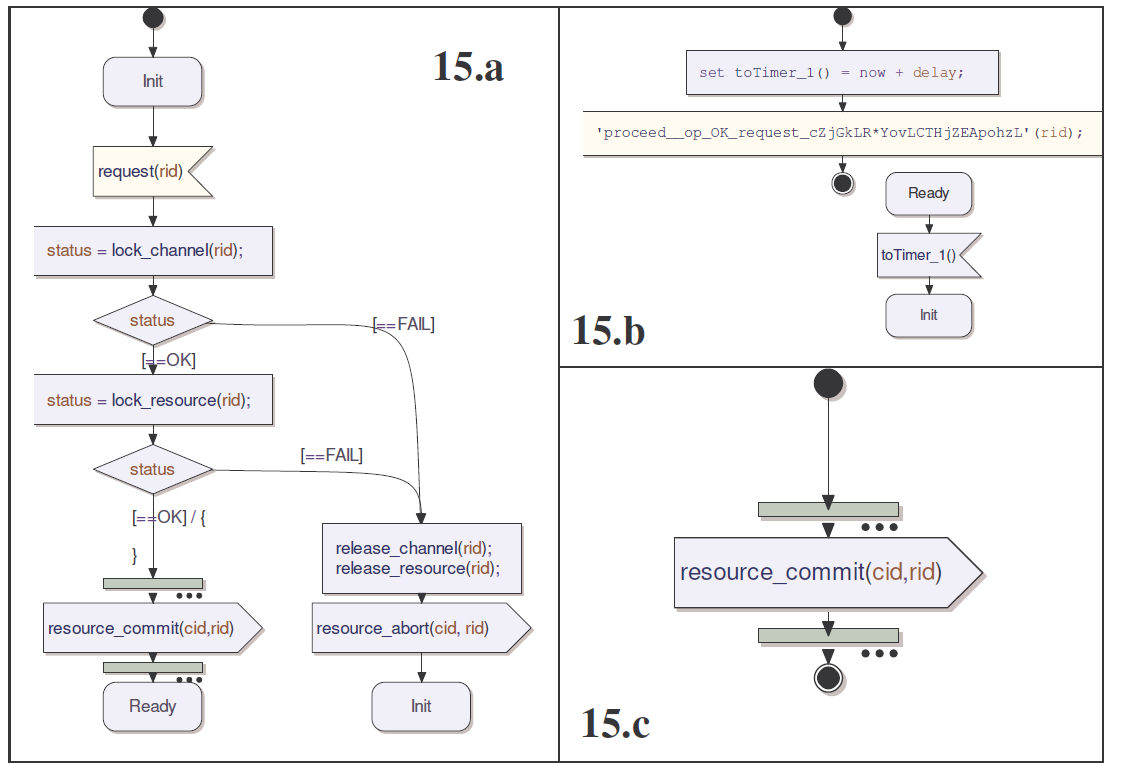
\includegraphics[width=475px]{img/weavr_composed.png}
	\caption{Visualização da composição do aspecto
	para controle de tempo no tratador de requisições.}\label{fig:weavr_composed}
\end{figure}

Motorola WEAVR também disponibiliza uma ferramenta para executar modelos de aspectos. Ao encontrar um conector, a ferramenta executa a máquina de
estado referente ao mesmo e retorna o controle a máquina de estado base. A possibilidade de executar um modelo de aspectos facilita a compreensão do
fluxo de execução de um programa orientado a aspectos. O trabalho de Cottenier estende a segunda versão da UML através de um perfil UML para
representar aspectos com diagramas de classes e diagramas de máquina de estados. Esta extensão pode ser importada em diferentes ferramentas CASE. 
Diagramas de classes permitem representar a parte estrutural de um sistema. Os diagramas de máquinas de estado são responsáveis por representar a
dinâmica do sistema. Motorola WEAVR permite representar a maior parte das características de programas orientados a aspectos, como \textit{wildcards}, 
pontos de corte, avisos, introduções e dependência entre aspectos. A ferramenta também disponibiliza ferramental para visualização, composição e 
execução de modelos de aspectos. Este ferramental é uma das principais contribuições do trabalho, pois automatiza parte do processo de modelagem e
permite gerar código em um linguagem alvo.

Uma limitação desta proposta, em relação a linguagem, é que apenas avisos do tipo durante (\textit{around}) são suportados. Outra desvantagem é o baixo nível 
de abstração dos modelos. Isto acontece, pois um dos focos do trabalho é a execução do sistema em nível de modelo, deixando os modelos  próximos do
nível de código. Os diagramas de máquinas de estado desta proposta contém trechos de código e código referente a POA, como chamadas ao método \textit{proceed()}. 
O baixo nível de abstração dificulta a compreensão dos modelos, pois o desenvolvedor precisa compreender chamadas próximas do nível de código. A
utilização de diagramas como os diagramas de caso de uso e de sequência permitiriam representar um sistema em um maior nível de abstração, facilitando a compreensão 
e manutenção do mesmo. 

\section{Modelagem de Aspectos com Diagramas de Sequência Proposto por Klein}

O trabalho de Klein \cite{Klein:2007:WMA:1805812.1805819} \cite{Klein:2006:SWS:1119655.1119662} propõe uma extensão aos diagramas de sequência da UML para permitir a modelagem
de sistemas orientados a aspectos. Esta extensão é realizada no meta-modelo da UML, estendendo o mesmo com a adição de novas classes, restrições e
relacionamentos. Separam-se os diagramas de sequência em dois tipos:

\begin{itemize}
  \item \textbf{bSD}: Diagrama de sequência básico que descreve um número finito de interações entre um conjunto de objetos. É equivalente ao diagrama
  de sequência padrão da UML.
  \item \textbf{cSD}: Diagrama de sequência composto que permite compor diagramas de sequência básicos através de operadores como nodos decisão
  e iterações. Este tipo de diagrama permire representar comportamentos infinitos e é semelhante ao diagrama de visão geral de interação.
\end{itemize}

O meta-modelo para diagramas de sequência pode ser visualizado na figura \ref{fig:klein_meta_model}. Observa-se a presença de duas classes que
derivam da super classe \textbf{SD}(\textit{SequenceDiagram}): \textbf{bSD}(\textit{BasicSequenceDiagram}) e
\textbf{cSD}(\textit{ComposedSequenceDiagram}). Um diagrama de sequência composto contém um conjunto de nodos e um conjunto de transições que estão
associadas a diagramas de sequência básicos.

\begin{figure}
	\centering
	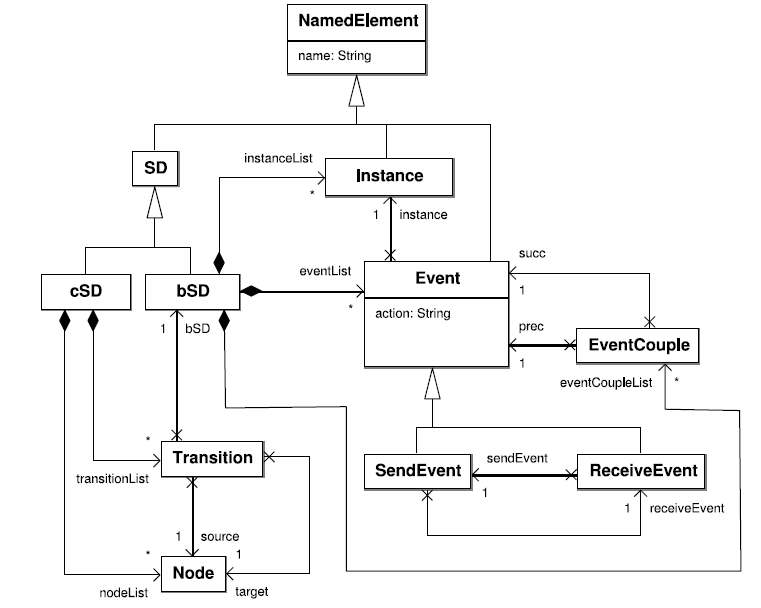
\includegraphics[width=475px]{img/klein_meta_model.png}
	\caption{Meta-modelo de extensão aos diagramas de
	sequência da UML}\label{fig:klein_meta_model}
\end{figure}

No lado esquerdo da figura \ref{fig:klein_sequence_diagrams} estão dispostos quatro bSD's: \textit{Propose}, \textit{Accept}, \textit{Retry} e
\textit{Rejected}. Estes bSD's representam etapas na interação com um servidor para realizar a autenticação de um usuário(\textit{log in}). O cSD
central e o cSD a direita são equivalentes e compõem os quatro bSD's a esquerda. Ambos cSD's especificam a autenticação de usuário(\textit{log in}). O
cSD central utiliza nodos decisão e o cSD a direita utiliza fragmentos do tipo \textit{alt} para representar diferentes caminhos de execução.

\begin{figure}
	\centering
	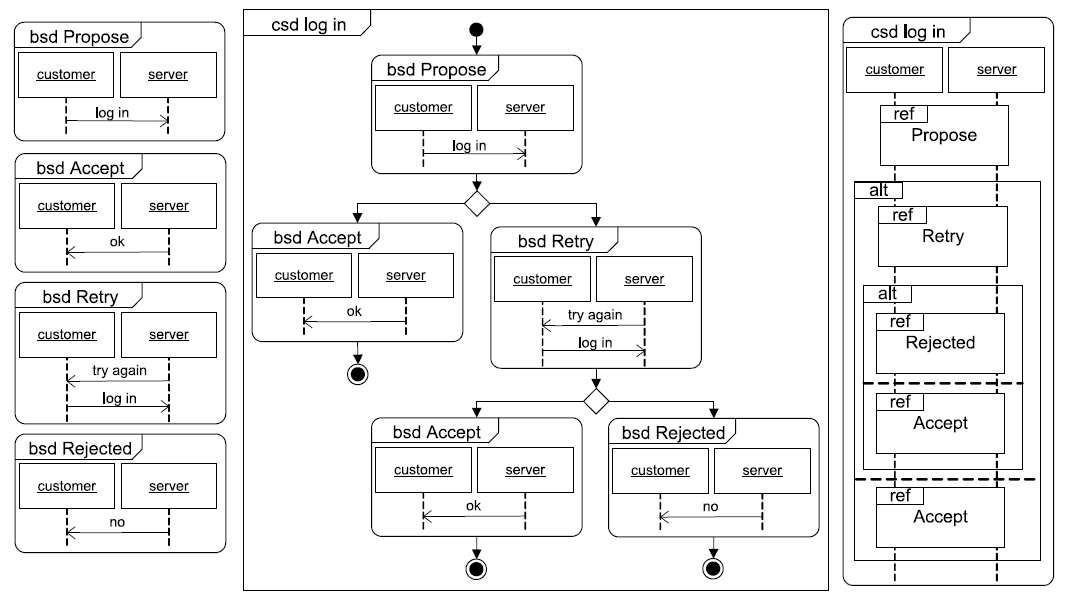
\includegraphics[width=475px]{img/klein_sequence_diagrams.png}
	\caption{Exemplos de diagramas de sequência
	estendidos: bSD's e cSD's}\label{fig:klein_sequence_diagrams}
\end{figure}

Para modelagem de aspectos deve-se definir um \textbf{aspecto comportamental} que é composto por dois bSD's: um para representar o ponto de corte e
outro para representar o novo comportamento (aviso). Um ponto de corte é representado como uma sequência de mensagens entre um conjunto de objetos. A
ferramenta não suporta a utilização de \textit{wildcards} na definição de pontos de corte, uma funcionalidade importante da POA, que permite a captura
de múltiplos pontos de junção em uma única declaração. Um aviso também é representado com bSD's e pode ser executado antes, durante ou depois dos
pontos de junção capturados por um ponto de corte. A figura \ref{fig:klein_aspects} mostra três aspectos comportamentais: registro de mensagens,
segurança e atualização de interface gráfica. O aspecto de segurança(\textit{Aspect Security}) define um ponto de corte que captura a troca das
mensagens \textit{log in} e \textit{try again} entre os objetos \textit{customer} e \textit{server}. O aviso que implementa o comportamento do aspecto
de segurança adiciona a mensagem \textit{save bad attempt} entre as mensagens \textit{log in} e \textit{try again}. Uma limitação nesta abordagem é
que o diagrama de sequência dos avisos é redundante, pois repete as mensagens capturadas no ponto de corte. No exemplo do aspecto de segurança, as
mensagens \textit{log in} e \textit{try again} são repetidas no aviso. Assim, se o ponto de corte for modificado, o aviso também deve ser modificado,
gerando um re-trabalho desnecessário. Na linguagem AspectJ, a modificação de um ponto de corte não gera modificações aos avisos associados aquele
ponto de corte.

\begin{figure}
	\centering
	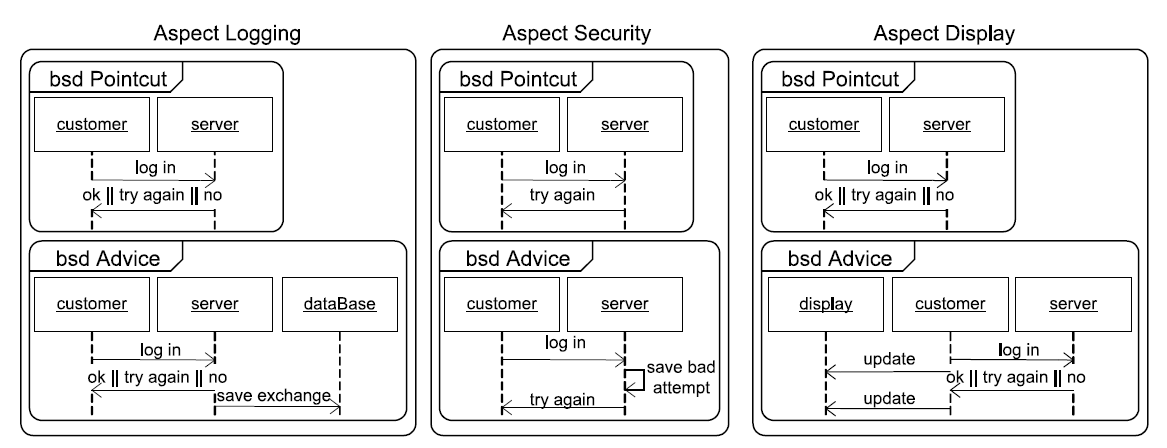
\includegraphics[width=475px]{img/klein_aspects.png}
	\caption{Exemplos de aspectos comportamentais}\label{fig:klein_aspects}
\end{figure}

Após definir os aspectos, deve-se realizar a composição dos aspectos em um modelo núcleo. O foco deste proposta é a composição de múltiplos aspectos
em um mesmo ponto de junção. Na composição de aspectos, o primeiro aspecto que for composto pode modificar a sequência de mensagens entre objetos no
modelo núcleo, fazendo com que o próximo aspecto não detecte o ponto de junção no qual o novo comportamento deveria ser inserido. Considerando a
composição entre o diagrama de sequência (cSD) \textit{log in} da figura \ref{fig:klein_sequence_diagrams} como modelo núcleo e os aspectos para
registro de mensagens, segurança e atualização de interface. Se o aspecto de segurança for o primeiro a ser composto, ele mudará a sequência de
mensagens entre os objetos \textit{customer} e \textit{server}, adicionando a mensagem \textit{save bad attempt} entre as mensagens \textit{log in} e
\textit{try again}. Se não existir um tratamento no algoritmo de detecção de pontos de junção,  os aspectos de registro de mensagens e atualização de
interface não capturarão os pontos de junção definidos por seus pontos de corte e a composição não será realizada corretamente. Assim, o algoritmo de
detecção de pontos de junção deve ser capaz de capturar pontos de junção, mesmo que existam mensagens introduzidas por outros aspectos durante a
composição de aspectos. A proposta de Klein resolve este problema detectando mensagens inseridas por outros aspectos durante a composição
de aspectos e permitindo a composição de múltiplos aspectos em um mesmo ponto de junção. A composição entre os aspectos e o modelo núcleo pode ser
visualizada na figura \ref{fig:klein_composition}.

\begin{figure}
	\centering
	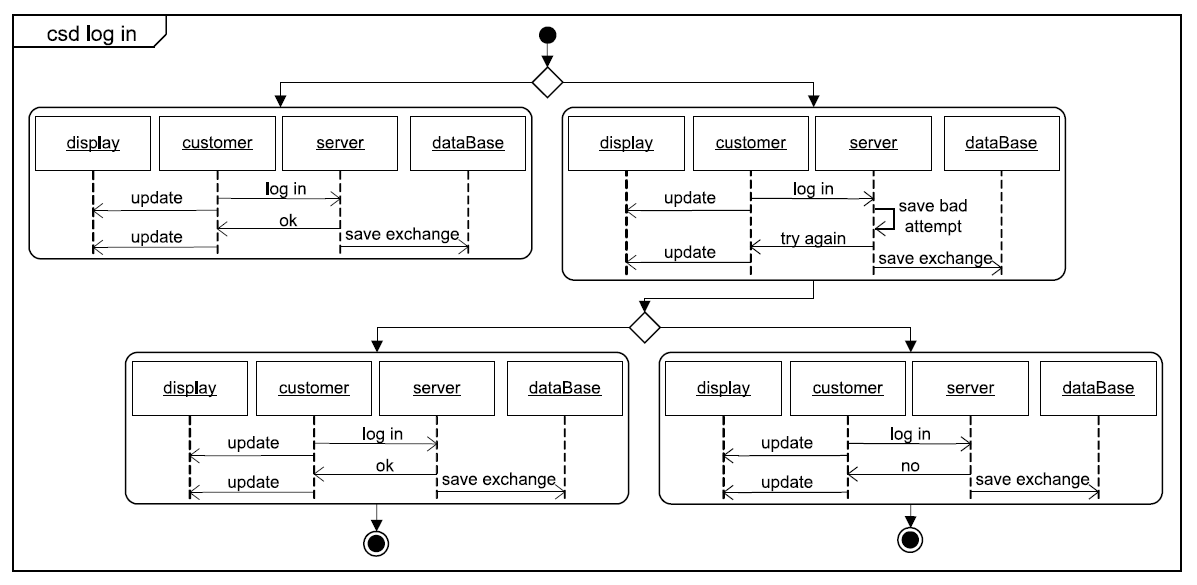
\includegraphics[width=475px]{img/klein_composition.png}
	\caption{Composição entre aspectos de registro de mensagens, segurança e 
	atualização de interface gráfica com modelo
	base para autenticação de usuário}\label{fig:klein_composition}
\end{figure}

Uma das limitações da proposta de Klein é a não representação da estrutura do sistema. A abordagem de Klein utiliza apenas diagramas de sequência para
modelagem da dinâmica do sistema. Em relação a POA, não é possível representar introduções de membros em classes, uma funcionalidade importante da
linguagem. Não é possível utilizar \textit{wildcards} na definição de pontos de corte, o que torna difícil a captura de múltiplos pontos de junção em
um mesmo ponto de corte. Além disso, a especificação de avisos contém redundâncias, pois replicam-se as mensagens referentes ao ponto de corte
capturado. A principal contribuição do trabalho é a possibilidade de realizar a composição de múltiplos aspectos em um mesmo ponto de junção, mantendo
as mensagens disparadas em cada aviso e identificando corretamente os pontos de junção, mesmo com mensagens introduzidas após a introdução de um
aviso. Em relação a forma de extensão à UML, as modificações da proposta não podem ser usadas diretamente em qualquer ferramenta CASE. Os modelos
gerados por esta proposta devem ser convertidos para o meta-modelo padrão da UML (através de transformações). A conversão de modelos não é tratada
neste trabalho, dificultando ainda mais o reuso da proposta em diferentes ferramentas CASE.

\section{Theme/UML Proposto por Clarke}

A proposta de Clarke \cite{clarke:04} permite realizar a análise e projeto de sistemas orientados a aspectos, desde a eliciação de requisitos,
passando pela modelagem e automatizando parte do processo com a composição automatizada de modelos núcleo com modelos de interesses entrecortantes
(aspectos). Na proposta elaborada por Clarke cada funcionalidade do sistema é considerada um tema (\textit{theme}). Os temas são identificados na fase
de levantamento de requisitos pela ferramenta Theme/Doc, que guia a obtenção de requisitos de sistemas orientados a aspectos. Para modelagem
estrutural utilizam-se os diagramas de pacote e de classes. Um pacote que representa um tema está associado ao estereótipo \textit{theme}, 
que representa um interesse do sistema. Diagramas de sequência são utilizados para modelagem comportamental. A modelagem de interesses
núcleo é realizada dentro dos padrões da UML, apenas marcando o pacote que define o tema com o estereótipo \textit{theme}. No entanto, a modelagem dos
interesses entrecortantes utiliza um mecanismo estendido de \textit{templates} da UML, que permite definir elementos não instancializados em um tema. 
Estes parâmetros serão instancializados posteriormente indicando quais elementos do modelo núcleo serão estendidos pelos interesses
entrecortantes. 

\begin{figure}
	\centering
	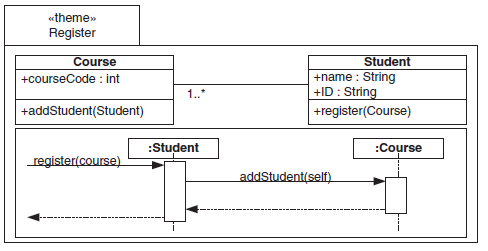
\includegraphics{img/theme_1.png}
	\caption{Modelo núcleo: registro de estudante em curso}\label{fig:theme_1}
\end{figure}

A figura \ref{fig:theme_1} apresenta um interesse núcleo para matrícula de um estudante em um curso. Observa-se a presença do estereótipo
\textit{theme} associado ao pacote que contém um diagrama de classes e um diagrama de sequência. A figura \ref{fig:theme_2} representa um interesse
entrecortante para registro de atividades do sistema, como o cadastro de um estudante em um determinado curso. Este tema contém um \textit{template}
UML com dois parâmetros. O primeiro parâmetro é o objeto do modelo núcleo que está sendo registrado e o segundo representa o método que está sendo
executado no modelo núcleo. Para realizar a composição de interesses, o desenvolvedor deve instancializar estes parâmetros com elementos do modelo
núcleo.

\begin{figure}
	\centering
	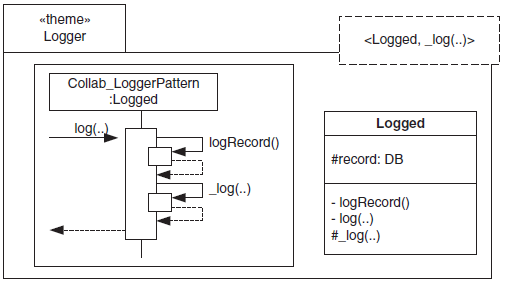
\includegraphics{img/theme_2.png}
	\caption{Modelo entrecortante: registro de atividades do sistema}\label{fig:theme_2}
\end{figure}

A figura \ref{fig:theme_3} apresenta uma configuração para composição de temas. Esta configuração define que objetos do tipo \textit{Person},
\textit{Student} e \textit{Professor} são objetos que podem ser alvo do registro de atividades. Além disso, define que os métodos que terão a
atividade registrada são: \textit{Student.register()}, \textit{Person.unregister()} e \textit{Professor.giveMark()}. Em relação a composição de
modelos, um plug-in para o ambiente de desenvolvimento Eclipse \cite{Eclipse} permite realizar a composição de modelos. O algoritmo de composição
recebe a modelagem em formato XMI como entrada e, baseado no meta-modelo proposto por Theme/UML, produz um modelo final independente de plataforma com
os modelos núcleo compostos com os interesses entrecortantes \cite{Carton:2009:MT:1692821.1692829}. 

\begin{figure}
	\centering
	\includegraphics{img/theme_3.png}
	\caption{Configuração de composição entre interesses}\label{fig:theme_3}
\end{figure}

Uma importante contribuição da abordagem é a especificação de aspectos desde a eliciação de requisitos, passando pela modelagem até a composição de
modelos. As ferramentas Theme/DOC e Theme/UML também permitem realizar a rastreabilidade de interesses (temas), desde a fase de requisitos, modelagem 
até o projeto do sistema. Outra vantagem da abordagem de Clarke é a independência de plataforma em relação a linguagem para programação orientada a
aspectos. Theme/UML é projetado como uma abordagem independente de plataforma, com mapeamentos para AspectJ, AspectWerkz \cite{aspectwerkz} e Hyper/J
\cite{hyperj}.

Uma das limitações da proposta de Clarke é a forma de extensão à UML, pois a mesma estende o meta-modelo da UML. Esta forma de extensão limita o uso
da proposta de modelagem apenas em ferramentas próprias. O meta-modelo depende da versão 1.3 \textit{beta} da UML e não pode ser utilizado em
ferramentas CASE que suportem a importação de perfis. Com o objetivo de inserir a abordagem dentro dos padrões da segunda versão da UML, foi
desenvolvido um perfil UML baseado na versão 2.1 da linguagem \cite{Carton:2009:MT:1692821.1692829}. No entanto, este trabalho ainda depende do meta-modelo 
original, pois para realizar a composição deve-se transformar os estereótipos e valores rotulados para o meta-modelo original do Theme/UML. 

\section{Modelagem de Aspectos com Diretivas de Composição Proposto por France}

O trabalho de France \cite{france:06} \cite{FranceReddy} apresenta uma proposta para especificação e composição de modelos de aspecto com modelos
núcleo utilizando diretivas de composição. Os modelos de aspecto são descrições genéricas de interesses entrecortantes, que devem ser instancializadas antes de serem
compostas com um modelo núcleo. A instancialização ocorre através de \textit{templates} da UML, semelhante a abordagem proposta por Clarke
\cite{clarke:04}. Um modelo de aspecto pode ser instancializado mais de uma vez na mesma modelagem. A instancialização de um modelo de aspecto envolve 
atribuir valores a todos os parâmetros de um \textit{template} com valores do domínio da aplicação. Um diferencial da proposta de Clarke é que a
comparação entre elementos do modelo para realizar a composição de classes utiliza outras variáveis além do nome do elemento, como o tipo de retorno
de um método, o número e o tipo dos parâmetros, etc. A comparação e seleção de elementos impactados é baseada em uma assinatura ao invés de uma
simples comparação por nome.

Além da comparação de elementos pela sua assinatura, a proposta também disponibiliza as diretivas de composição, que permitem adicionar restrições e
verificações para a composição de modelos. Existem dois tipos de diretivas: de modelo e de elemento. As diretivas de modelo definem a ordem de
composição de modelos, isto é, a ordem que os aspectos são compostos. Já as diretivas de elemento determinam como um modelo de aspecto é composto em
um modelo núcleo. Um exemplo de diretiva de elemento é a adição de novos elementos em um modelo. Estes elementos são definidos em um modelo de aspecto
e devem ser inseridos no modelo composto. Já um exemplo de diretiva de modelo é a definição de precedência entre aspectos no momento da composição.
Esta diretiva especifica que um modelo de aspecto deve ser composto antes de outro modelo.

A figura \ref{fig:clarke_1} exemplifica o uso de diretivas de composição. O modelo núcleo a esquerda apresenta duas classes: \textit{Writer} e
\textit{FileStream}, que representam o comportamento de escrever linhas em um \textit{stream}. O modelo de aspecto a direita contém as mesmas duas
classes e adiciona uma outra classe para introduzir um \textit{buffer} de escrita (\textit{WriterBuffer}). Para realizar a composição entre estes dois
modelos deve-se adicionar algumas diretivas de composição. A primeira diretiva é a remoção da associação entre as classes \textit{Writer} e
\textit{FileStream}, pois agora a escrita passará por um \textit{buffer}. Além disso, remove-se a especificação Object Constraint Language (OCL)
\cite{ocl:12} do método \textit{writeLine()} no modelo primário. A remoção da especificação OCL e da associação entre classes podem ser visualizadas
na figura \ref{fig:clarke_2}, que mostra os modelos após a aplicação das diretivas de composição. Após a aplicação das diretivas, a composição de modelos pode ser realizada sem disparar conflitos entre
os elementos dos modelos.

As diretivas de composição são uma importante contribuição da proposta de France, pois elas permitem realizar a composição de diagramas de classe
prevendo e evitando a maior parte dos conflitos. O foco deste trabalho é a especificação e a composição da estrutura de aspectos. A parte
comportamental é tratada pelo trabalho de Reddy e Solberg \cite{ReddySolberg}, que estende a proposta e trata da especificação e composição 
de diagramas de sequência. No entanto, a composição de diagramas de sequência e a adição de um suporte ferramental para a composição dos mesmos ainda estão
sendo estudadas pelos autores. O trabalho de France e Reddy \cite{FranceReddy} estuda a implementação de uma ferramenta para composição dos modelos
estruturais automaticamente, sem esforço do desenvolvedor. Este suporte ferramental é importante, pois automatiza parte do processo de modelagem,
diminuindo a quantidade de esforço manual necessária.

Uma das limitações da proposta de \cite{france:06} é a não representação de algumas características importantes da POA, como a captura de múltiplos
pontos de junção em uma única construção. A abordagem utiliza \textit{templates} da UML para instancializar os aspectos com elementos do domínio da
aplicação, mas não permite instancializar múltiplos elementos ao mesmo tempo. Outra limitação da abordagem é a falta de suporte ferramental para
realizar a composição de modelos comportamentais. Os modelos devem ser compostos manualmente pelo desenvolvedor. O suporte ferramental automatiza
parte do processo de modelagem, diminuindo o esforço do desenvolvedor e o tempo necessário para realizar a modelagem. A composição de modelos
comportamentais permite visualizar o efeito do comportamento dos modelos entrecortantes (aspectos) nos modelos núcleos, facilitando a compreensão de
um sistema orientado a aspectos.

\begin{landscape}
\begin{figure}
	\centering
	\includegraphics{img/clarke_1.png}
	\caption{Antes do uso de diretivas de composição para composição de aspectos}\label{fig:clarke_1}
\end{figure}
\end{landscape}

\begin{landscape}
\begin{figure}
	\centering
	\includegraphics{img/clarke_2.png}
	\caption{Depois do uso de diretivas de composição para composição de aspectos}\label{fig:clarke_2}
\end{figure}
\end{landscape}

\section{Modelo de Projeto de Aspectos (AODM) Proposto por Stein}

A proposta de Stein (Aspect-Oriented Design Model (AODM)) \cite{stein:02} \cite{Stein02onrepresenting} \cite{stein:aosd-uml02} permite a especificação
de sistemas orientados a aspectos. A modelagem é baseada nas construções da linguagem AspectJ para implementação de aspectos utilizando Java. O
trabalho de Stein estende o meta-modelo da UML através de um perfil UML, adicionando estereótipos e valores rotulados. No entanto, algumas
construções estendem o meta-modelo da UML diretamente. Segundo os autores, propõe-se também uma composição em nível de modelo das construções
propostas pela linguagem AspectJ. A modelagem de aspectos é implementada utilizando diagrama de classes, colaborações da UML 1.x e casos de uso. Os
casos de uso são utilizados para definir a ordem de composição entre aspectos. A proposta permite a composição de aspectos e de introduções.

Para representar aspectos adiciona-se o estereótipo \textit{aspect} ao elemento do meta-modelo \textit{(Class)}. Um aspecto contém alguns parâmetros
de configuração, atributos, operações, pontos de corte e avisos. Pontos de corte são definidos com o estereótipo \textit{pointcut}, que 
estende \textit{(Operation)} e contém uma assinatura e uma declaração. A declaração define quais pontos de junção serão capturados nos modelos
núcleo. O estereótipo \textit{advice} também estende o elemento do meta-modelo \textit{Operation} e permite especificar avisos. 
Introduções são especificadas utilizando \textit{templates} da UML.  O estereótipo \textit{introduction} permite representar introduções de métodos,
classes, atributos e também de relacionamentos entre elementos. Antes de utilizar um \textit{template} que define uma introdução deve-se instancializar 
todos os parâmetros com argumentos do domínio de aplicação. 

O exemplo da figura \ref{fig:stein_1} apresenta um modelo de aspecto (AODM) segundo a proposta de Stein. O exemplo trata do padrão de projeto
observador/observado que permite que um observador escute mudanças em alguns objetos observados. A modelagem contém um aspecto abstrato que deve ser
estendido e um aspecto concreto que implementa o padrão de projeto. O aspecto abstrato (\textit{SubjectObserverProtocol}) contém um aviso do tipo
depois e um ponto de corte. O ponto de corte \textit{stateChanges} captura mudanças no estado de um objeto e deve ser especificado pelo aspecto
concreto. A semântica adicionada pelo aspecto abstrato é que os objetos observadores serão notificados quando ouver alguma mudança de estado nos
objetos observados. No entanto, o exemplo não apresenta como é modelado o comportamento do aviso. O aspecto concreto
(\textit{SubjectObserverProtocolImpl}) instancializa o padrão de projeto em uma aplicação, sobreescrevendo o ponto de corte \textit{stateChanges} para 
capturar cliques em um botão. Além disso, adiciona duas introduções às classes \textit{Button} e \textit{ColorLabel}. 

\begin{figure}
	\centering
	\includegraphics{img/stein_1.png}
	\caption{Um modelo de aspecto segundo a abordagem AODM}\label{fig:stein_1}
\end{figure}

Uma das limitações da proposta de Klein é a necessidade de estender o meta-modelo da UML. Embora a proposta utilize um perfil UML para adicionar estereótipos e valores rotulados, o meta-modelo da
UML é estendido. A extensão do meta-modelo não permite que a proposta seja utilizada em qualquer ferramenta CASE que suporte a importação de perfis.
Outra limitação do trabalho é a dependência com a primeira versão da UML, com o uso de diagramas de colaboração, que dependem de construções presentes
na primeira versão da linguagem. A falta de uma ferramenta para composição automática de modelos é outra limitação do trabalho, pois é necessário que o desenvolvedor
especifique todos os modelos manualmente, inclusive os modelos compostos.

\section{Comparação de Abordagens}

Existem algumas abordagens para modelagem de sistemas orientados a aspectos. Esta dissertação propõe uma comparação entre diferentes abordagens
considerando alguns critérios de comparação. Os critérios apresentados na próxima sessão são baseados no trabalho proposto por Wimmer
\cite{wimmer:2011:SUA:1978802.1978807}. A próxima seção apresenta os critérios propostos por este trabalho. Para permitir uma
melhor visualização das tabelas de comparação, as abordagens são abreviadas com as três primeiras letras do autor principal. 
Para cada critério, apresenta-se a tabela de comparação entre as abordagens e uma pequena discussão sobre os resultados de
cada tabela.

\subsection{Critérios Propostos por Wimmer}

\subsubsection{Critérios de Linguagem}

\begin{itemize}
	\item \textbf{Linguagem para Modelagem (L.M)}: Diz respeito a linguagem utilizada para modelagem. Neste trabalho apenas abordagens que utilizam UML
	são estudadas. Logo, abordagens podem utilizar a versão 1.x ou a segunda versão da UML.
	\item \textbf{Mecanismo de Extensão (M.E)}: Abordagens para modelagem de sistemas orientados a aspectos podem estender a UML através de um perfil
	leve, que pode ser utilizado em ferramentas CASE que suportem a importação de perfis, ou adicionando novos elementos, restrições e relacionamentos ao
	meta-modelo da linguagem. A extensão através de perfis permite uma maior inter-operabilidade de abordagens para modelagem em diferentes ferramentas
	CASE \cite{Booch:2005:UML:1088874}.
	\item \textbf{Diagramas Estruturais (D.E)}: Quais diagramas estruturais são utilizados para descrever a estrutura de aspectos.
	\item \textbf{Diagramas Comportamentais (D.C)}: Quais diagramas comportamentais são utilizados para descrever o comportamento de aspectos.
\end{itemize}

A tabela \ref{tab:comparison_table_language} apresenta a comparação entre diferentes abordagens utilizando os critérios de linguagem.

\begin{table*}[h]
	\centering
	\begin{tabular}{ | c | c | c | c | c | c | c | c | c | c | }
		\hline
		 & KLE & EVE & KIE & JAC & CUI & STE & COT & CLA & GHI \\
		\hline
		 L.M & 2.0 & 2.0 & 2.0 & 2.0 & 2.0 & 1.x & 2.0 & 2.0 (1.x) & 2.0 \\
		\hline
		 L.E & MM & P & P & MM & P & MM & P & MM & P \\
		\hline
		 D.E & - & DC & DC & DC, DComp & - & DC & DC, DEC, DI & DP, DC & DP, DC\\
		\hline
		 D.C & DS & - & DS, DME & DS, DCom, DCU & DA & DCol & DME & DS & DS, DME \\
		\hline
	\end{tabular}
	
	\hspace{2em}

	\begin{tabular}{  p{16.6cm}  }
		Abreviações Autores: \\
	\end{tabular}
	
	\begin{tabular}{ | p{16.6cm} | }
		\hline
		KLE (Klein), EVE (Evermann), KIE (Kienzle), JAC (Jacobson), CUI (Cui), STE (Stein), COT (Cottenier), CLA (Clarke), GHI (Ghilardi) \\
		\hline
	\end{tabular}
	
	\begin{tabular}{  p{16.6cm}  }
		Legenda: \\
	\end{tabular}

	\begin{tabular}{ | p{16.6cm} | }
		\hline
		MM (Meta-Modelo), P (Perfil UML), DC (Diagrama de Classes), DComp (Diagrama de Componentes), DEC (Diagrama de Estrutura Composta), DI
		(Diagrama de Implantação), DP (Diagrama de Pacotes), DS (Diagrama de Sequência), DCol (Diagrama de Colaboração), DA (Diagrama de Atividades), 
		DME (Diagrama de Máquina de Estados), DCU (Diagrama de Casos de Uso) e DCom (Diagrama de Comunicação)\\
		\hline
	\end{tabular}
	\caption{Comparação entre abordagens: critérios de linguagem}
	\label{tab:comparison_table_language}
\end{table*} 

Observa-se que a maior parte das abordagens especificam aspectos com a segunda versão da UML. As abordagens limitadas a primeira versão da UML não contemplam todas 
as construções da linguagem e, não são suportadas por qualquer ferramenta CASE, diminuindo a expressividade da abordagem e a qualidade da mesma. Em
relação a forma de extensão, algumas abordagens estendem por um perfil UML, enquanto outras estendem diretamente o meta-modelo. A extensão por meta-modelo 
não permite utilizar a abordagem em outra ferramenta diferente da que foi implementada 
originalmente, diminuindo o potencial de reuso. Já um perfil UML pode ser importado em ferramentas CASE que suportem a importação de perfis,
possibilitando o reuso em ferramentas CASE comerciais. A maior parte das abordagens utiliza diagramas de classe para modelagem estrutural. Em relação
ao comportamento, a maior parte das abordagens modela com diagramas de sequência. Na especificação comportamental, alguns abordagens utilizam o
diagrama de máquina de estados, que permite representar em mais detalhes o comportamento de sistemas orientados a aspectos, como a modelagem de pontos
de corte.

\subsubsection{Critérios de Composição e Modelos}

\begin{itemize}
	\item \textbf{Composição Simétrica (C.S)}: Este critério analisa quais modelos de interesses podem ser compostos com outros modelos. Na modelagem de
	sistemas orientados a aspectos, em algumas abordagens, o modelo do interesse entrecortante (aspecto) é modelado diferentemente do modelo núcleo.
	Nesses casos, a composição é assimétrica, pois apenas modelos de interesses entrecortantes podem ser compostos em modelos núcleo. A composição
	simétrica acontece quando não há diferenciação entre modelos entrecortantes e modelos núcleo, podendo realizar a composição entre qualquer modelo.
	\item \textbf{Nível de Abstração (N.A)}: Distingue o nível de abstração dos elementos das abordagens. As abordagens podem representar construções de
	sistemas orientados a aspectos em alto ou baixo nível de abstração. É possível que uma abordagem represente conceitos nos dois níveis.
	\item \textbf{Composição Estrutural (C.E)}: Avalia se a abordagem permite realizar a composição estrutural de modelos.
	\item \textbf{Composição Comportamental (C.C)}: Avalia se a abordagem permite realizar a composição do comportamento de modelos.
	\item \textbf{Ferramenta para Modelagem (F.M)}: Distingue abordagens que disponibilizam uma ferramenta para modelagem, de abordagens que não
	disponibilizam uma ferramenta que auxilie a modelagem. Abordagens que estendem a UML através de um perfil automaticamente disponibilizam este suporte, pois o perfil
	pode ser importado em outras ferramentas CASE.
	\item \textbf{Ferramenta para Composição (F.C)}: Algumas abordagens disponibilizam uma ferramenta para composição automática da estrutura e
	comportamento de modelos, possibilitando visualizar o comportamento de aspectos inserido no sistema, sem esforço do desenvolvedor. 
\end{itemize}

A tabela \ref{tab:comparison_table_models} apresenta a comparação entre diferentes abordagens utilizando os critérios de composição e modelos.

\begin{table*}[h]
	\centering
	\begin{tabular}{ | c | c | c | c | c | c | c | c | c | c | }
		\hline
		 & KLE & EVE & KIE & JAC & CUI & STE & COT & CLA & GHI \\
		\hline
		 C.S & sm & - & asm & asm & asm & asm & asm & sm & asm \\
		\hline
		 N.A & alto & baixo & alto & alto & alto & baixo & baixo & alto & alto \\
		\hline
		 C.E & não & sim & sim & não & não & sim & sim & sim & sim \\
		\hline
		 C.C & sim & não & sim & não & sim & não & sim & sim & sim \\
		\hline
		 F.M & não & sim & sim & não & não & não & sim & sim & sim \\
		\hline
		 F.C & não & não & não & não & não & não & sim & não & sim  \\
		\hline
	\end{tabular}
	
	\hspace{2em}

	\begin{tabular}{  p{12cm}  }
		Abreviações Autores: \\
	\end{tabular}
	
	\begin{tabular}{ | p{12cm} | }
		\hline
		KLE (Klein), EVE (Evermann), KIE (Kienzle), JAC (Jacobson), CUI (Cui), STE (Stein), COT (Cottenier), CLA (Clarke), GHI (Ghilardi) \\
		\hline
	\end{tabular}

	\begin{tabular}{  p{12cm}  }
		Legenda: \\
	\end{tabular}

	\begin{tabular}{ | p{12cm} | }
		\hline
		sm (Modelos Simétricos), asm (Modelos Assimétricos) \\
		\hline
	\end{tabular}
	\caption{Comparação entre abordagens: critérios de composição e modelos}
	\label{tab:comparison_table_models}
\end{table*} 

Em relação à modelagem simétrica ou assimétrica, a maior parte das abordagens especifica os interesses entrecortantes com construções diferentes dos
interesses núcelo. A maior parte das abordagens representa aspectos em alto nível de abstração. A modelagem em alto nível de abstração facilita a
compreensão e manutenção do sistema. Boa parte das abordagens permite a modelagem de sistemas orientados a aspectos. Abordagens que estendem a
linguagem através de um perfil podem ser utilizadas em outras ferramentas CASE, possibilitando a modelagem sem a necessidade de implementar uma
ferramenta específica. Algumas abordagens suportam a composição estrutural e comportamental, que podem ser realizadas através de um procedimento
algorítmico. No entanto, apenas a proposta de Cottenier e a abordagem proposta por esta dissertação disponibilizam ferramentas para realizar 
a composição de modelos automaticamente. O uso de ferramentas que automatizam parte do processo de modelagem é uma importante contribuição, pois
diminuem o tempo de modelagem de um sistema.

\subsubsection{Critérios de Pontos de Junção e Aviso}

\begin{itemize}
	\item \textbf{Modelo de Ponto de Junção (M.PJ)}: Este critério distingue entre duas formas possíveis de especificar pontos de junção: de maneira
	explícita, identificando quais elementos da linguagem podem representar pontos de junção; de maneira implícita, utilizando o próprio modelo de pontos de junção
	da linguagem para programação orientada a aspectos (POA).
	\item \textbf{Representação de Ponto de Corte (R.PC)}: Distingue a forma de representação de pontos de corte, a qual pode ser textual ou gráfica,
	com algum diagrama da linguagem. 
	\item \textbf{Composição de Ponto de Corte (C.PC)}: Avalia se a abordagem permite realizar a composição de pontos de corte, com os operadores
	lógicos AND e OR. 
	\item \textbf{Representação de Aviso (R.A)}: Avalia se a representação de avisos (antes, durante ou depois) é realizada.
\end{itemize}

A tabela \ref{tab:comparison_table_join_points_advices} apresenta a comparação entre diferentes abordagens utilizando os critérios de pontos de
junção e avisos.

\begin{table*}[h]
	\centering
	\begin{tabular}{ | c | c | c | c | c | c | c | c | c | c | }
		\hline
		 & KLE & EVE & KIE & JAC & CUI & STE & COT & CLA & GHI \\
		\hline
		 M.PJ & exp & imp & exp & imp & exp & imp & exp & imp & exp  \\
		\hline
		 R.PC & gra & tex & gra & tex & gra & tex & gra & tex & gra \\
		\hline
		 C.PC & sim & sim & sim & sim & sim & sim & sim & sim & sim \\
		\hline
		 R.A & sim & sim & sim & sim & sim & sim & sim & sim & sim \\
		\hline
	\end{tabular}
	
	\hspace{2em}
	
	\begin{tabular}{  p{11cm}  }
		Abreviações Autores: \\
	\end{tabular}
	
	\begin{tabular}{ | p{11cm} | }
		\hline
		KLE (Klein), EVE (Evermann), KIE (Kienzle), JAC (Jacobson), CUI (Cui), STE (Stein), COT (Cottenier), CLA (Clarke), GHI (Ghilardi) \\
		\hline
	\end{tabular}
	
	\begin{tabular}{  p{11cm}  }
		Legenda: \\
	\end{tabular}

	\begin{tabular}{ | p{11cm} | }
		\hline
		exp (Explícita), imp (Implícita), tex (Textual), gra (Gráfica)  \\
		\hline
	\end{tabular}
	\caption{Comparação entre abordagens: critérios de ponto de junção e avisos}
	\label{tab:comparison_table_join_points_advices}
\end{table*} 

Algumas abordagens representam explicitamente o modelo de pontos de junção, selecionando elementos da própria linguagem para representar os pontos de
junção da POA. Um exemplo é o uso do diagrama de sequência para representar pontos de junção, onde uma mensagem representa a chamada de um método, por
exemplo (utilizado na abordagem de Klein). Já a representação implícita, na maior parte das vezes, é uma representação textual de alguma linguagem
para programação de aspectos, como AspectJ. Esta dissertação representa pontos de corte com o diagrama de máquina de estados, utilizando elementos do diagrama 
para representação dos pontos de junção. Algumas abordagens representam pontos de corte diagramaticamente, enquanto outras representam apenas
textualmente. A representação diagramática facilita a compreensão dos modelos, opção desta dissertação. Todas as abordagens permitem a composição de
pontos de corte e a representação de avisos.

\subsection{Critérios Propostos por Ghilardi}

Os seguintes critérios são propostos por esta dissertação para comparação de modelagens para sistemas orientados a aspectos:

\subsubsection{Critérios de Especificação de Aspectos e de Visualização}

\begin{itemize}
	\item \textbf{Representação de Introduções (R.I)}: Avalia se a abordagem permite especificar introduções de elementos em um modelo núcleo,
	adicionando um novo método, atributo ou modificando a hierarquia de herança de classes que especificam um interesse núcleo.
	\item \textbf{Captura de Múltiplos Pontos de Junção (C.M.PJ)}: Distingue quais abordagens
	permitem a captura de múltiplos pontos de junção de maneira praticável, com o uso de expressões regulares (\textit{wildcards}).
	\item \textbf{Alternância de Visões (A.V)}: Avalia se a abordagem permite realizar a alternância de visões, visualizando ora o comportamento dos
	interesses entrecortantes (aspectos), dos interesses núcleo, ou, a composição dos interesses entrecortantes com os interesses núcleos. Esta alternância de visões deve 
	ser realizada sem o esforço do desenvolvedor.
	\item \textbf{Efeito de Aspectos (E.A)}: Este critério distingue abordagens que permitem visualizar o efeito dos aspectos nos modelos finais,
	diferenciando os diferentes interesses no modelo composto.
	\item \textbf{Composição Automática de Pontos de Corte (C.A.PC)}: Avalia se a abordagem permite realizar a composição automática de pontos de corte,
	sem esforço do desenvolvedor.
\end{itemize}

A tabela \ref{tab:comparison_table_aspects_visualization} apresenta a comparação entre diferentes abordagens utilizando os critérios de aspectos e
visualização.

\begin{table*}[h]
	\centering
	\begin{tabular}{ | c | c | c | c | c | c | c | c | c | c | }
		\hline
		 & KLE & EVE & KIE & JAC & CUI & STE & COT & CLA & GHI \\
		\hline
		 R.I & não & não & sim & sim & não & sim & sim & sim & sim \\
		\hline
		 C.M.PJ & não & sim & sim & sim & sim & não & sim & sim & sim \\
		\hline
		 A.V & não & não & não & não & não & não & não & não & sim \\
		\hline
		 E.A & não & não & não & não & não & não & não & não & sim \\
		\hline
		 C.A.PC & não & não & não & não & não & não & não & não & sim \\
		\hline
	\end{tabular}
	
	\begin{tabular}{  p{11.5cm}  }
		Abreviações Autores: \\
	\end{tabular}
	
	\begin{tabular}{ | p{11.5cm} | }
		\hline
		KLE (Klein), EVE (Evermann), KIE (Kienzle), JAC (Jacobson), CUI (Cui), STE (Stein), COT (Cottenier), CLA (Clarke), GHI (Ghilardi) \\
		\hline
	\end{tabular}
	
	\caption{Comparação entre abordagens: critérios de aspectos e visualização}
	\label{tab:comparison_table_aspects_visualization}
\end{table*} 

O principal diferencial da abordagem proposta nesta dissertação é a possibilidade de realizar a alternância de visões dinamicamente, visualizando os
interesses entrecortantes, os interesses núcleo ou configurações de composição de interesses entrecortantes com interesses núcleo. O visualizador de
aspectos é disponibilizado através de uma ferramenta disponível no ambiente SEA. Este visualizador também permite visualizar o efeito dos aspectos no
sistema, através da diferenciação por cores no modelo composto. Apenas esta dissertação permite realizar a alternância de visões automaticamente,
visualizando o efeito dos aspectos no sistema. 

Outros critérios importantes não tratados pela pesquisa de Wimmer \cite{wimmer:2011:SUA:1978802.1978807} são: a modelagem de introduções, a captura de
múltiplos pontos de junção em uma mesma construção e a composição automática de pontos de corte. A abordagem proposta permite especificar introduções
utilizando os diagramas de classe da UML. A captura de múltiplos pontos de junção de maneira é realizada utilizando a linguagem AspectJ na definição
dos pontos de corte (especificados no diagrama de máquina de estados). Outra contribuição importante desta dissertação é a composição automática de
pontos de corte, através da composição de máquinas de estado. A composição automática de pontos de corte é outra contribuição deste
trabalho, pois não é tratada por nenhum outro trabalho na área de modelagem de sistemas orientados a aspectos.

\section{Discussão}

A maior parte das abordagens permite representar a estrutura e o comportamento de sistemas orientados a aspectos. No entanto, algumas construções
importantes da POA não são representadas por essas abordagens, como a representação de todos os tipos de avisos. Em algumas abordagens, as construções
são representáveis, mas demandam um esforço adicional do desenvolvedor. Um exemplo, é o esforço necessário para realizar a captura de múltiplos pontos
de junção, pois a maior parte das abordagens necessitam que cada elemento a ser capturado por um ponto de corte seja selecionado manualmente. Outra
limitação da maior parte das abordagens é a falta de ferramental para composição automática de modelos. Este suporte ferramental é importante na
etapa de modelagem, pois diminui o tempo de desenvolvimento e facilita a compreensão e manutenção dos modelos. A geração automática de modelos
compostos gera subsídios para realização da alternância de visões, visualizando o efeito dos aspectos no sistema.

Assim, não existe uma abordagem que represente todas as características de POA, automatizando parte do processo de modelagem, permitindo visualizar o
efeito dos aspectos no sistema. A abordagem proposta por esta dissertação tem como objetivo representar todas as características de sistemas
orientados a aspectos, estruturais e comportamentais, de maneira praticável, automatizando parte do processo de modelagem. Como produtos deste trabalho, destacam-se o
suporte para modelagem de aspectos no ambiente SEA, que também pode ser utilizado em outras ferramentas CASE que suportem a importação de
perfis; uma ferramenta que realiza a composição automática de modelos de interesses entrecortantes (aspectos) com modelos de interesses
núcleos, possibilitando a visualização do efeito dos aspectos no sistema.

O próximo capítulo apresenta a proposta para especificação de sistemas orientados a aspectos, com as características apresentadas neste capítulo, e
também apresenta o suporte ferramental para modelagem, composição e visualização dinâmica de aspectos.

\chapter{Especificação e Modelagem de Sistemas Orientados a Aspectos}

Este capítulo apresenta um Perfil UML para especificação de sistemas orientados a aspectos e uma ferramenta para realizar a composição de interesses
núcleo com interesses entrecortantes (aspectos). O perfil UML fornece subsídios para realizar a modelagem e a composição automática de modelos núcleo
com modelos entrecortantes. A ferramenta que realiza a composição de modelos, o algoritmo e o visualizador de aspectos são apresentados na parte
final deste capítulo.

\section{Especificação de Sistemas Orientados a Aspectos}

O meta-modelo padrão da UML não permite a especificação de todas as características de sistemas orientados a aspectos. Este trabalho define um perfil
UML que estende a linguagem com novas construções, permitindo a modelagem de sistemas que utilizam aspectos. Esta seção descreve os
estereótipos, valores rotulados e restrições propostas por este perfil e também apresenta uma abordagem para representação das características estruturais e
comportamentais de aspectos, fornecendo subsídios para composição automática de modelos de aspectos com modelos núcleo do sistema. A figura
\ref{fig:uml_profile} apresenta o perfil UML proposto para representar a estrutura e o comportamento de aplicações orientadas a aspectos.
Este perfil pode ser utilizado em ferramentas CASE que suportem a importação de perfis através do padrão XML Metadata Interchange (XMI) \cite{xmi:11} para
troca de meta-dados via Extensible Markup Language (XML). 

\subsection{Especificação Estrutural}

Para modelagem estrutural, este trabalho utiliza algumas definições do trabalho proposto por Evermann \cite{Evermann:2007:MSP:1229375.1229379}, o qual
permite a representação das características estruturais de aspectos. As definições usadas do perfil de Evermann são os 
estereótipos \textit{CrosscuttingConcern} e \textit{Aspect}, que estão com o fundo bege no diagrama de perfil da figura
\ref{fig:uml_profile}. Um estereótipo estende um elemento do meta-modelo da UML, adicionando uma nova semântica a um elemento do modelo. Neste
trabalho, um elemento do meta-modelo a ser estendido é representado dentro de parênteses. O estereótipo \textit{CrosscuttingConcern} estende
(\textit{Package}) e contém um conjunto de classes e aspectos, representando um interesse que impacta uma ou mais partes de um sistema. O estereótipo
\textit{Aspect} estende (\textit{Class}), contém declarações inter-tipos (introduções) e algumas propriedades de configuração, que são valores
rotulados. O primeiro valor rotulado é \textit{isPrivileged} que determina se um aspecto é privilegiado, isto é, se ele tem acesso a membros privados
de outras classes do sistema. Outra propriedade que pode ser configurada é o tipo de instancialização de um aspecto. O tipo de instancialização é
definido pelos valores rotulados \textit{perType} e \textit{perPointcut}. O valor rotulado \textit{perType} é um enumerável com quatro opções:
\textit{perthis}, \textit{pertarget}, \textit{percflow}, \textit{percflowbelow} e define o tipo de instancialização. O valor
rotulado \textit{perPointcut} define qual é o ponto de corte que está associado. Um exemplo de uso desta variável seria a instanciação do aspecto para
cada fluxo de execução após a captura de um ponto de corte. Esta instanciação poderia incluir o próprio ponto de corte (\textit{percflow}), ou não (\textit{percflowbelow}). 

As declarações inter-tipos permitem a injeção de membros (métodos, atributos) em classes, mudanças de hierarchia de herança entre classes e de
implementação de interfaces. Estas declarações também permitem a mudança de hierarquia de aspectos. Para representar declarações inter-tipos, foi
proposto o estereótipo \textit{ClassExtension}. Este estereótipo estende (\textit{Class}) e está associado a outro estereótipo denominado
\textit{Introduction}. O estereótipo \textit{Introduction} é usado para marcar quais membros estão sendo inseridos em uma classe, ou qual relacionamento de herança está sendo adicionado ou removido, ou qual interface está sendo implementada. O estereótipo
\textit{Introduction} estende os elementos do meta-modelo (\textit{Attribute}), (\textit{Operation}), (\textit{Generalization}) e
(\textit{Realization}).

\begin{figure} \centering
	\includegraphics{img/full_profile.png}
	\caption{Perfil UML para modelagem de sistemas orientados a aspectos}\label{fig:uml_profile}
\end{figure}

Com os estereótipos propostos e o diagrama de classes da UML, é possível representar a estrutura de aplicações orientadas a aspectos usando
pacotes, classes e aspectos. O exemplo da figura \ref{fig:structural_profile_example} mostra como modelar um interesse entrecortante usando o perfil
UML proposto por esta dissertação. Alguns dos exemplos apresentados são baseados no sistema de gerenciamento de hotéis proposto por Jacobson para
apresentar sua proposta de modelagem \cite{Jacobson:2004:ASD:1062430}. 

O interesse representado na figura \ref{fig:structural_profile_example} é a capacidade de um objeto ter seu estado copiado para outro objeto.
A funcionalidade \textit{Copyable} é especificada como um interesse entrecortante que contém o aspecto \textit{CopyableAspect}, duas extensões de classes e a definição da interface \textit{ICopyable}.
As classes \textit{Room} e \textit{Reservation} são marcadas com o estereótipo \textit{ClassExtension}, para sinalizar que estão sendo estendidas pelo aspecto. A primeira extensão adicionada as
classes é a implementação da interface \textit{ICopyable}, que define dois métodos para um objeto ter a capacidade de ser copiável. Como a interface
\textit{ICopyable} exige a implementação de dois métodos, o aspecto introduz os métodos \textit{copy()} e \textit{deepCopy()} nas classes \textit{Room} e \textit{Reservation}. 
A realização da interface \textit{ICopyable} em ambas as classes e os métodos introduzidos são marcados com o estereótipo \textit{Introduction}.

\begin{figure}[!b] \centering
	\includegraphics{img/structural_profile_example.png}
	\caption{Exemplo de modelagem estrutural: interesse entrecortante \textit{Copyable}}\label{fig:structural_profile_example}
\end{figure}

\subsection{Especificação Comportamental}

Além da especificação estrutural, com declarações inter=tipos e configurações de instancialização, deve-se especificar o comportamento de um aspecto.
Um aspecto é composto por pontos de corte e avisos, os quais definem em quais pontos e qual comportamento estenderá um sistema. O perfil de Evermann 
\cite{Evermann:2007:MSP:1229375.1229379} representa pontos de corte dentro da própria especificação de um aspecto, isto é, na representação estrutural
de um aspecto com classes. Esta forma de especificação não permite a captura de múltiplos pontos de junção em um mesmo ponto de corte, pois
apenas elementos da modelagem UML podem ser selecionados. A abordagem proposta nesta dissertação representa pontos de corte com o diagrama de máquina 
de estados da UML. Cada transição representa a captura de um ou mais pontos de junção, com a possibilidade de uso de expressões regulares
(\textit{wildcards}) para captura de múltiplos pontos de execução em uma mesma construção. Se a captura de todos os pontos de junção for 
satisfeita, isto é, se as condições para disparar uma transição forem satisfeitas, considera-se que o sistema satisfez um ponto de corte. A expressão
regular (\textit{wildcard}) definida nas transições entre estados segue o padrão proposto pela linguagem AspectJ. A composição de pontos de corte é
realizada através da composição de diferentes máquinas de estado, onde cada máquina de estado representa um ponto de corte. No perfil proposto, o
estereótipo \textit{StatePointcut} estende (\textit{State}) e representa um ponto de corte. A definição deste estereótipo pode ser visualizada na figura \ref{fig:uml_profile}.

A figura \ref{fig:pointcut_definition_1} mostra um exemplo de definição de um ponto de corte. O ponto de corte \textit{AnyCall} captura chamadas
(ponto de corte do tipo \textit{call}) a qualquer método, de qualquer classe, usando uma expressão regular (\textit{wildcard}) para capturar qualquer
tipo de retorno, qualquer classe e qualquer nome de método com qualquer número de parâmetros. O ponto de corte \textit{RoomTarget} captura a ocorrência de uma chamada
quando o objeto alvo (ponto de corte do tipo \textit{target}) é do tipo \textit{Room}. Cada ponto de corte é representado como um estado no diagrama
de máquina de estados. A assinatura de um ponto de corte é especificada na transição que leva ao estado do ponto de corte, a qual permite o uso de
\textit{wildcards} para capturar múltiplos pontos de junção. Quando um ponto de corte é satisfeito, significa que o sistema capturou os pontos de execução 
especificados pela assinatura do ponto de corte.

\begin{figure}[h]
	\centering
	\includegraphics{img/pointcut_definition_1.png}
	\caption{Definição de dois pontos de corte}\label{fig:pointcut_definition_1}
\end{figure}

A linguagem AspectJ permite a composição de pontos de corte com os operadores lógicos \textit{and} e \textit{or}. A abordagem proposta nesta
dissertação realiza a composição automática de pontos de corte usando o diagrama de máquina de estados. Os próximos exemplos apresentam a composição
de pontos de corte proposta por esta dissertação. A figura \ref{fig:pointcut_definition_and} apresenta a composição dos pontos de corte
\textit{AnyCall} e \textit{RoomTarget} usando o operator \textit{and}. A máquina de estado composta contém um estado com uma região concorrent, contendo 
sub-estados que executam concorrentemente: \textit{AnyCall} e \textit{RoomTarget}. A sincronização ocorre com os nodos \textit{fork} e \textit{join}, 
os quais garantem que o estado final (\textit{AnyCall AND RoomTarget}) somente será satisfeito se ambos os estados (\textit{AnyCall} e \textit{RoomTarget} 
forem satisfeitos. Esta é a semântica do operador \textit{and} na linguagem AspectJ. A figura
\ref{fig:pointcut_definition_or} apresenta a composição de pontos de corte usando o operador \textit{or}. Neste caso a semântica é um pouco diferente,
porque o sistema alcançara o estado final (\textit{AnyCall OR RoomTarget}) quando qualquer um dos pontos de corte for satisfeito. Este comportamento é
representado na máquina de estados composto, que contém transições diretas de ambos estados para o estado final.

\begin{figure}[h]
	\centering
	\includegraphics{img/pointcut_definition_and.png}
	\caption{A composição de dois pontos de corte com o operador AND}\label{fig:pointcut_definition_and}
\end{figure}

Um ponto de corte captura somente os pontos de execução de um sistema. O comportamento que deve ser injetado nestes pontos é representado pelo aviso,
o qual está diretamente associado a um ponto de corte. Diagramas de sequência são utilizados para representar o comportamento dos interesses núcleo
(modelo núcleo) e dos interesses entrecortantes (modelos entrecortantes). Um aspecto pode conter um ou mais avisos e cada um é representado por um
modelo entrecortante. O comportamento de um aviso executa quando os pontos de corte associados ao mesmo são satisfeitos, isto é, todos os pontos de
junção são capturados. Como nesta dissertação pontos de corte são modelados com o diagrama de máquina de estados e avisos com o diagrama de sequência,
a conexão entre avisos com pontos de corte deve ser realizada utilizando elementos sintáticos destes diagramas. A conexão entre estes elementos é
realizada através do uso de invariantes de estado. Uma invariante de estado é um fragmento de interação associado com a linha de vida de um diagrama
de sequência, representado uma restrição em tempo de execução nos participantes da interação. A alcançabilidade de um estado é usado como restrição
para disparar a execução de um aviso. 

\begin{figure}[!hb]
	\centering
	\includegraphics{img/pointcut_definition_or.png}
	\caption{A composição de dois pontos de corte com o operador OR}\label{fig:pointcut_definition_or}
\end{figure}

A definição de um modelo entrecortante (como um diagrama de sequência) inicia adicionando o aspecto como o elemento associado a primeira linha de vida
do diagrama. Uma invariante de estado, a qual representa a satisfação do ponto de corte, é associada a linha de vida do aspecto. Isto significa que a
sequência de mensagens ocorrerá somente quando o sistema atingir o estado representado pela invariante de estado. As mensagens podem ser executados
antes, durante ou depois do disparo do ponto de corte. O tempo de execução das mensagens adicionadas pelo aspecto é configurado usando o estereótipo
\textit{AdviceExecutionType}. Este estereótipo estende (\textit{StateInvariant}) e é apresentado na parte inferior da figura \ref{fig:uml_profile}. O
estereótipo \textit{AdviceExecutionType} tem um valor rotulado do tipo enumeração denominado de \textit{adviceType}. Os tipos válidos para este enumerável são:
antes, durante ou depois.

\begin{figure}
	\centering
	\includegraphics{img/behavioral_profile_example.png}
	\caption{A conexão entre pontos de corte e avisos usando invariantes de estado}\label{fig:behavioral_profile_example}
\end{figure}

A conexão entre pontos de corte e avisos pode ser melhor compreendida no exemplo da figura \ref{fig:behavioral_profile_example}. A figura
\ref{fig:behavioral_profile_example} apresenta o ponto de corte previamente especificado para captura de chamadas (ponto de corte \textit{call}) de
qualquer método em qualquer classe com qualquer número de parâmetros (\textit{AnyCall}). O aspecto de registro de mensagens (\textit{log}) define um
modelo entrecortante que registra uma mensagem usando uma classe do tipo \textit{Logger}. O modelo entrecortante é descrito como uma sequência de
mensagens em uma diagrama de sequência. Este diagrama contém uma invariante de estado que referencia o ponto de corte \textit{AnyCall}. Uma invariante
de estado deve ter o estereótipo \textit{AdviceExecutionType} e o valor rotulado \textit{adviceType} para especificar quando o comportamento do aviso
será executado. No exemplo, o comportamento do aspecto será eecutado depois (\textit{after}) dos pontos de junção capturados pelo ponto de corte
\textit{AnyCall}. A mensagem \textit{log()} será executada somente quando o estado \textit{AnyCall} for satisfeito.


\section{Visualização e Composição Automatizada de Aspectos}

Esta seção apresenta a ferramenta \textit{SEA/Aspect} que é um dos produtos do esforço de pesquisa relatado nesta dissertação, a qual permite a
visualização de modelos entrecortantes compostos com modelos núcleo utilizando diagramas de classe e de sequência. O algoritmo para composição de 
modelos é descrito em passos para realizar a composição de classes e de mensagens. Finalmente, o visualizador de aspectos é apresentado.

\subsection{A Ferramenta SEA/Aspect}

O perfil UML proposto fornece subsídios para composição e visualização dinâmica de aspectos. O perfil foi adicionado no ambiente de desenvolvimento
SEA \cite{silva:00}, o qual suporta a diagramação e modelagem UML. A ferramenta SEA/Aspect permite a seleção de quais modelos entrecortantes serão
compostos com os modelos núcleo do sistema. Um desenvolvedor pode automaticamente visualizar somente os modelos núcleo, os modelos entrecortantes, ou
os modelos núcleo compotos com os entrecortantes. Aspectos podem ser habilitados ou desabilitados dinamicamente, atualizando o modelo composto. Esta
atualização automática permite a mudança de visões, visualizando diferentes composições de modelos.

  \begin{figure}[!h]
	\centering
	\includegraphics{img/selection_screen.png}
	\caption{Seleção de modelos para composição}\label{fig:selection_screen}
  \end{figure}

A composição de modelos da ferramenta SEA/Aspect tem dois passos para produzir um modelo composto: \textbf{seleção} e \textbf{composição},
as quais são descritas nas próximas duas seções. A fase de seleção deve ser executada manualmente pelo desenvolvedor, enquanto a fase de composição é
executada automaticamente pelo algoritmo de composição do ambiente SEA.

\subsubsection{Seleção}
  
Nesta etapa o desenvolvedor seleciona manualmente quais modelos núcleo e entrecortantes deseja compor atribuindo uma cor diferente para cada modelo.
Estas cores diferenciam os elementos de cada modelo no modelo composto. As mensagens enviadas pelos objetos de cada modelo serão preenchidas com a cor
associada ao modelo em questão. A figura \ref{fig:selection_screen} apresenta a janela para seleção de aspectos na ferramenta SEA/Aspect. Neste
exemplo é possível visualizar três modelos entrecortantes: lista de espera (\textit{Waiting List}), registro de mensagens (\textit{Log}) e
programa de fidelidade (\textit{Earn Loyalty Points}) e um modelo núcleo: reserva de quarto (\textit{ReserveRoom}). Nesta seleção, o desenvolvedor
deseja visualizar a composição entre os modelos \textit{ReserveRoom}, \textit{Waiting List} e \textit{Log}.
  
Os modelos núcleo e entrecortantes selecionados pelo desenvolvedor são utilizados como entrada da etapa de composição, que, basedo nos pontos de corte
e nas introduções dos modelos entrecortantes selecionará quais elementos devem ser modificados no modelo composto.  

\subsubsection{Composição}

A composição é realizada entre um modelo núcleo e um ou mais modelos entrecortantes, provendo como resultado um modelo composto com a estrutura ou o
comportamento dos modelos entrecortantes injetados no modelo núcleo. No modelo composto, o comportamento entrecortante diferencia-se do comportamento
núcleo pelas cores diferentes, como pode ser visualizado na figura \ref{fig:case_study_compound_2}, que mostra a composição de diagrama de
sequência entre os interesses de lista de espera, reserva de quarto e registro de mensagens de um sistema.

O meta-modelo do ambiente de desenvolvimento SEA \cite{silva:00} é utilizado para composição de modelos. Os principais elementos do meta-modelo podem ser
visualizados no diagrama da figura \ref{fig:sea_meta_model}. No meta-modelo do SEA, uma especificação (\textit{Specification}) agrega um conjunto de elementos de
especificação (\textit{SpecificationElement}), os quais podem ser modelos (\textit{ConceptualModel}) ou conceitos (\textit{Concept}). Estes modelos
de especificação podem ser associados com dois tipos de relacionamento: sustentabilidade (\textbf{sustainment}) e referência (\textbf{reference}). O
relacionamento de sustentabilidade estabelece uma relação semântica entre dois elementos, quando um assume o papel de sustentado e o outro de
sustentador. A semântica desse relacionamento é que o elemento sustentado existirá em uma especificação enquanto o elemento sustentador existir.
Um exemplo de relacionamento de sustentabilidade é o relacionamento entre classes, atributos e métodos, no qual uma classe é o sustentador e seus
campos são sustentados pela classe. O relacionamento de referência estabelece que elementos referenciadores dependem de um elemento referenciado. Um
exemplo deste tipo de relacionamento é uma mensagem em um diagrama de sequência, que depende de um método de uma determinada classe. Se o método for
removido da especificação, a mensagem ainda existirá, mas sua semântica estará incompleta.

  \begin{figure}[!h]
	\centering
	\includegraphics{img/sea_meta_model.png}
	\caption{Meta-modelo do ambiente SEA \cite{silva:00}}\label{fig:sea_meta_model}
  \end{figure}

É possível realizar um mapeamento do meta-modelo do ambiente SEA para o meta-modelo da UML. Cada elemento do meta-modelo da UML é representado por um
conceito e os diagramas da UML são os modelos. Um diagrama da UML contém um conjunto de elementos, os quais podem estar associados. Na linguagem do
SEA, um modelo contém um cojunto de conceitos com relacionamentos de referência ou sustentabilidade. Por exemplo, o diagrama de classe é um modelo que
contém conceitos como classe, atributo e método. O diagrama de sequência também é um modelo e contém conceitos como linha de vida, mensagem,
invariante de estado, etc.
  
Com a definição do mapeamento entre os elementos do meta-modelo SEA para o meta-modelo da UML, é necessário uma classe que implemente o algoritmo de
composição: a classe \textit{AspectComposer}. O algoritmo de composição tem duas atividades: \textbf{match} e \textbf{merge}. A primeira atividade
localiza os conceitos selecionados no modelo núcleo pelos pontos de corte ou introduções definidas nos modelos entrecortantes. A atividade de \textit{merge} 
injeta a estrutura ou o comportamento dos modelos entrecortantes no modelo núcleo, fornecendo como resultado um modelo composto. A ferramenta
SEA/Aspect permite a composição automática de diagramas de classe e de sequência.

A composição de diagramas de classe faz uma comparação por nome para selecionar os elementos impactados e tem os seguintes passos:
  
\begin{itemize}
  
	\item \textbf{Comparação e Seleção:} Utiliza uma estratégia que compara diretamente o nome entre aspectos, classes, atributos e métodos. O algoritmo
	procura por elementos que estejam associados com o estereótipo \textit{ClassExtension} nos modelos entrecortantes. Um conceito marcado com este
	estereótipo contém introduções (com o estereótipo \textit{Introduction}) para serem adicionadas em outros conceitos. Essas introduções podem ser a
	adição de campos (métodos ou atributos), mudança na hierarquia de herança ou a implementação de uma interface. 
	
	\item \textbf{Composição:} Quando os conceitos impactados são localizados, o compositor executa uma operação de composição entre os modelos
	entrecortantes e o modelo núcleo. Esta composição produz um modelo composto com os campos, relacionamentos de generalização e realização
	adicionados aos conceitos impactados no modelo núcleo. Esta operação de composição é realizada utilizando o meta-modelo do ambiente SEA, o qual
	permite a adição, remoção e modificação de relacionamentos entre conceitos dinamicamente.

\end{itemize}

A figura \ref{fig:structural_composition_example} apresenta um modelo composto originado pela composição de dois modelos estruturais (diagramas de
classe). O primeiro diagrama é modelado na figura \ref{fig:structural_profile_example} e apresenta o interesse entrecortante que adiciona a
funcionalidade de um objeto ter seu estado copiado para outro objeto utilizando a interface \textit{ICopyable}. O interesse núcleo é modelado pelo diagrama na figura
\ref{fig:structural_core_concern_class_diagram} e modela a estrutura de classes necessária para realizar a reserva de um quarto de hotel. Este
modelo contém a classe \textit{Room} com o método \textit{updateAvailability()} e a classe \textit{ReserveRoomHandler} com o
método \textit{makeReservation()}. O algoritmo de composição de diagrama de classes começa selecionando elementos do modelo núcleo que são
impactados pelos modelos entrecortantes (comparação direta por nome). Neste primeiro filtro, verifica-se que somente a classe \textit{Room} está
presente em ambos os modelos, logo, esta classe pode ter alguma mudança na sua estrutura. Verifica-se que a classe \textit{Room} está marcada com o 
estereótipo \textit{ClassExtension}, o que significa que a mesma sofrerá a introdução de algum membro presente no modelo entrecortante. O próximo
passo do algoritmo é buscar por estereótipos do tipo \textit{Introduction}. Ao executar este passo, seis estereótipos são encontrados, sendo dois
que adicionam um relacionamento de realização de interface entre as classes \textit{Room} e \textit{Reservation} com a nova interface
\textit{ICopyable}, e quatro estereótipos que adicionam os métodos \textit{copy()} e \textit{deepCopy()} nas classes \textit{Room} e
\textit{Reservation}. Neste exemplo de composição, apenas a classe \textit{Room} será modificada pelas introduções do modelo entrecortante. Ao final, 
o modelo composto contém a classe \textit{Room} com dois novos métodos: \textit{copy()} e \textit{deepCopy()} e implementando a interface \textit{ICopyable}. 
A classe \textit{ReserveRoomHandler} não foi modificada com a composição, pois o modelo entrecortante não introduz nenhuma modificação para esta
classe.

  \begin{figure}[!h]
	\centering
	\includegraphics{img/structural_core_concern_class_diagram.png}
	\caption{Modelo núcleo para reserva de quarto}\label{fig:structural_core_concern_class_diagram}
  \end{figure}
    
  \begin{figure}[!h]
	\centering
	\includegraphics{img/structural_composition_example.png}
	\caption{Composição do modelo núcleo com o modelo entrecortante para cópia de estado entre objetos}\label{fig:structural_composition_example}
  \end{figure}

A composição de diagramas de sequência realiza a comparação entre conceitos utilizando expressões regulares (\textit{wildcard matching}) e tem os
seguintes passos:
  
	\begin{itemize}
	  
	  \item \textbf{Comparação e Seleção:} Com os modelos núcleo e entrecortantes selecionados pelo desenvolvedor, o algoritmo de composição busca pelos
	  pontos de junção do modelo núcleo que são impactados pelos pontos de corte definidos nos modelos entrecortantes. A busca pode ser separada em três
	  passos:
	  
	  \begin{enumerate}

	    \item \textbf{Obtenção do Ponto de Corte:} Para obter o ponto de corte do diagrama de sequência do interesse entrecortante (modelo
	    entrecortante), o algoritmo busca por invariantes de estado com o estereótipo \textit{AdviceExecutionType}. Este tipo de invariante de estado
	    está associada a um estado que define um ponto de corte.

	    \item \textbf{Separação do Ponto de Corte:} O algoritmo de composição de aspectos utiliza uma expressão regular para separar o ponto de corte em
	    quatro partes: \textbf{tipo de ponte de corte}, \textbf{padrão de tipo de retorno}, \textbf{padrão de identificação} e \textit{padrão de
	    exceção}. O tipo de ponto de corte é mandatório e pode ser um dos tipos suportados pela linguagem AspectJ, os quais incluem \textit{execution},
	    \textit{this}, \textit{target}, \textit{call}, entre outros. O padrão de tipo de retorno é opcional e especifica o tipo de retorno de um ponto de
	    corte. Um método pode retornar um objeto de um determinado tipo, pode não ter nenhum retorno ou pode aceitar qualquer tipo de retorno. O padrão
	    de identificação também é mandatório e contém a assinatura do conceito que deve ser comparada e encontrada no modelo núcleo. Um exemplo de padrão
	    de identificação é a captura de todos os métodos que começam com a palavra \textit{update}. Finalmente, o padrão de exceção é opcional e é
	    utilizado para capturar os pontos de execução os quais lançam exceção de algum tipo especificado pelo padrão.
	    
	    \item \textbf{Comparação e Seleção de Pontos de Junção:} A estratégia de composição utiliza expressões regulares para comparar e selecionar
	    quais pontos de junção são impactados pelos pontos de corte definidos nos modelos entrecortantes. Esta comparação suporta pontos de corte
	    especificados através de \textit{wildcards}, que é uma importante funcionalidade das linguagens para programação orientada a aspectos. O
	    algoritmo começa utilizando o padrão de identificação para encontrar o contexto no qual os conceitos impactados estão envolvidos, como o pacote e
	    a classe de um dado método, por exemplo. Quando todos os conceitos dentro de um dado contexto são capturados, o algoritmo utiliza outra expressão
	    regular para selecionar os nomes dos conceitos capturados. Por exemplo, ao comparar e selecionar um método, o algoritmo verifica o tipo de
	    retorno, os parâmetros (nome, tipo e número de parâmetros) e a assinatura do método. Finalmente, o algoritmo verifica se alguma exceção é
	    lançada. Como saída, os conceitos (classes e métodos) impactados pelos modelos entrecortantes são armazenados para serem usados posteriormente na
	    atividade de composição.
	  \end{enumerate}  
	  
	  \item \textbf{Composição:} Esta etapa compõe os conceitos dos modelos entrecortantes com os conceitos dos modelos núcleo selecionados. O algoritmo
	  recebe como entrada os conceitos impactados do modelo núcleo que devem ser compostos com conceitos dos modelos entrecortantes. O objetivo desta
	  atividade é a injeção de um conjunto de mensagens, linhas de vida, fragmentos combinados e outros elementos do diagrama de sequência no diagrama de
	  sequência núcleo (modelo núcleo), adicionando comportamento definido nos diagramas de sequência dos interesses entrecortantes (modelos
	  entrecortantes). O ambiente SEA facilita a composição de conceitos, como a adição ou remoção de mensagens entre objetos, adição de novos objetos em
	  um diagrama de sequência, etc. O algoritmo de injeção de mensagens entre modelos pode ser separado em dois passos:
	  
		  \begin{enumerate}
		    
		    \item \textbf{Obtenção do Tipo de Execução do Aviso:} Obtém-se o tipo de execução do aviso a partir do valor rotulado da invariante de estado
		    selecionada. Os tipos de aviso suportados são: antes, durante e depois e os mesmos são definidos pelo valor rotulado \textit{adviceType}. O tipo
		    de aviso fornece informações de quando as mensagens serão executadas no diagrama de sequência núcleo.

		  	\item \textbf{Injeção de Mensagens:} Neste momento, o algoritmo já sabe quais são os conceitos impactados, as mensagens a serem injetadas do
		  	modelo entrecortante no modelo núcleo e em qual ponto do tempo as mensagens devem ser injetadas. O próximo passo é a injeção de mensagens e o
		  	reordenamento do diagrama de sequência, pois a injeção de uma mensagem dispara um evento de reordenamento. Com todas as mensagens injetadas e
		  	ordenadas, o algoritmo modifica a cor de fundo de cada mensagem com a cor associada ao respectivo interesse entrecortante, para diferenciar quais
		  	mensagens são provenientes de qual aspecto. A composição produz como saída um diagrama de sequência composto com os conceitos entrecortantes
		  	compostos no diagrama de sequência núcleo.
		  
		  \end{enumerate}
		  
	  \end{itemize}  
	  
\subsubsection{Ordem de Precedência}

A composição de modelos entrecortantes em um modelo núcleo pode gerar diferentes resultados dependendo da ordem de precedência dos interesses. É
possível definir a ordem de precedência entre aspectos utilizando a linguagem AspectJ, com o objetivo de determinar qual aspecto tem precedência
perante outro aspecto ou perante todos os outros aspectos do sistema. Logo, uma abordagem para especificação e modelagem de sistemas orientados a
aspectos deve fornecer uma maneira de tornar determinística a composição de modelos. O problema de precedência ocorre quando em aspectos diferentes,
pontos de corte impactam o mesmo ponto de junção. A linguagem não consegue determinar as mensagens de qual aspecto terão preferência e serão compostas
primeiro. A ordem de precedência envolve os três tipos de aviso: antes, durante ou depois e tem as seguintes regras:

\begin{enumerate}
  \item \textbf{Antes:} Um aspecto com maior precedência executa seus avisos do tipo antes em um ponto de junção antes de outros aspectos com menor
  precedência.
  \item \textbf{Depois:} Um aspecto com maior precedência executa seus avisos do tipo depois em um ponto de junção depois de outros aspectos com menor
  precedência.
  \item \textbf{Durante:} Um aspecto com maior precedência executa seus avisos do tipo durante antes de outros aspectos com menor precedência. Além
  disso, este aspecto tem o controle de permitir a execução de outros avisos ou não.
\end{enumerate}

  \begin{figure}[!h]
	\centering
	\includegraphics{img/log_aspect.png}
	\caption{Definição da aspecto para registro de mensagens}\label{fig:log_aspect}
  \end{figure}
  \
  \begin{figure}[!h]
	\centering
	\includegraphics{img/auth_aspect.png}
	\caption{Definição da aspecto para autenticação}\label{fig:auth_aspect}
  \end{figure}

O Perfil UML proposto por esta dissertação adiciona o valor rotulado \textit{precedence} ao estereótipo \textit{Aspect}. Este valor rotulado define a
ordem de precedência entre aspectos. O tipo deste valor rotulado é um texto, que contém o nome dos aspectos os quais terão a precedência definida.
É possível utilizar expressões regulares na declaração de precedência de aspectos para especificar que um determinado aspecto deve preceder qualquer
outro aspecto do sistema, ou, que um determinado aspecto deve ter menor prioridade do que qualquer outro aspecto. A ordem de precedência é maior da
esquerda para a direita na definição de aspectos. Aspectos com a mesma ordem de precedência, ou sem ordem de precedência definida, serão compostos
seguindo a ordem de especificação dos modelos na modelagem.

A seguir apresenta-se um exemplo de definição de precedência entre dois aspectos: um aspecto para
registro de mensagens (que pode ser visualizado na figura \ref{fig:log_aspect}) e outro aspecto para autenticação de usuário, apresentado 
na figura \ref{fig:auth_aspect}. O aspecto de autenticação de usuário tem maior precedência ao aspecto de registro de mensagens. Para definir essa 
restrição na modelagem, o aspecto de autenticação atribui o valor \textit{'AuthAspect, LogAspect'} ao valor rotulado \textit{precedence}. Esta
definição representa que as modificações estruturais e comportamentais propostas pelo aspecto \textit{AuthAspect} terão precedência perante as 
modificações do aspecto de registor de mensagens \textit{LogAspect}.

\subsubsection{Visualizador de Aspectos}

O perfil UML e o algoritmo de composição implementado na ferramenta SEA/Aspect permitem o intercâmbio de visões de diferentes interesses em
uma modelagem. A visualização do comportamento dos aspectos (interesses entrecortantes) nas funcionalidades núcleo de um sistema facilita a
compreensão e a manutenção de sistemas orientados a aspecto nas primeiras fases de desenvolvimento, permitindo que o desenvolvedor compreenda a ordem de execução do
sistema observando modelos. Um dos obstáculos das abordagens orientadas a aspectos é a dificuldade de compreensão do sistema, já que é difícil
entender o fluxo de execução sem ferramentas adicionais. O visualizador pode ser utilizado na etapa de modelagem, permitindo compreender o sistema em
um mais alto nível de abstração. 

O visualizador de aspectos permite selecionar um interesse núcleo e um conjunto de interesses entrecortantes para serem visualizados em um mesmo
modelo. O objetivo principal deste visualizador é verificar como fica o comportamento do sistema após a adição de um ou mais aspectos. Sem o
auxílio do visualizador, o efeito dos aspectos só pode ser visualizado ao executar o sistema, ou, utilizando ferramentas adicionais para visualização
em nível de código.

A figura \ref{fig:case_study_compound_1} apresenta um modelo composto, que permite a visualização do efeito de um aspecto para registro de mensagens
(\textit{log}) em um interesse para reserva de quartos de um sistema de gerenciamento de hotel. Esta configuração de visões é uma composição
entre o interesse para reserva de quarto e o interesse de registro de mensagens. Observa-se nesta composição que as mensagens do interesse para reserva de 
quartos (\textit{makeReservation()} e \textit{updateAvailability()}) não estão com nenhuma cor de fundo. Já a mensagem do interesse de registro de
mensagens (\textit{log()}) está com o fundo vermelho, pois foi a cor associada a este interesse. Esta diferenciação é importante para diferenciar quais mensagens 
vem de qual interesse no modelo composto. As mensagens que estão com a cor vermelha são provenientes do aspecto para registro de mensagens, logo,
estas mensagens representam o efeito do aspecto no sistema principal. Observa-se um seletor de modelos na parte inferior esquerda do diagrama de
sequência composto. Este seletor permite selecionar quais interesses são visualizados em uma mesma composição. Assim, é possível visualizar o efeito
de um ou mais aspectos ao mesmo tempo. 

O próximo capítulo apresenta dois estudos de caso que detalham a composição e visualização de um ou mais interesses entrecortantes (aspectos) em um
mesmo interesse núcleo.

\begin{landscape}
  \begin{figure*}[]
	\centering
	\includegraphics{img/case_study_compound_1.png}
	\caption{Reserva de quarto composto com registro de mensagens}\label{fig:case_study_compound_1}
  \end{figure*}
\end{landscape}
\chapter{Estudo de Caso}\label{case_study}

Este cap�tulo apresenta dois estudos de caso para verificar a aplicabilidade da abordagem proposta na modelagem de interesses de uma aplica��o. Os
estudos de caso s�o baseados no sistema para gerenciamento de hotel proposto por Jacobson \cite{Jacobson:2004:ASD:1062430}. Este exemplo possibilita a
modelagem de importantes funcionalidades de aspectos e foi utilizado para validar a abordagem de Jacobson. Os casos de uso tratados pelos
estudos de caso s�o: reserva de quartos, tratamento de uma lista de espera para clientes, registro de mensagens, \textit{check-out} de clientes e o
ac�mulo de pontos em um programa de fidelidade. 

Os estudos de caso tratam da composi��o autom�tica de modelos comportamentais, isto �, da composi��o de diagramas de sequ�ncia. O algoritmo de
composi��o para diagramas de sequ�ncia utiliza estere�tipos e valores rotulados dos diagramas de classe. Por este motivo, modela-se tamb�m a
estrutura dos interesses de cada estudo de caso. Diagramas de sequ�ncia s�o utilizados para representar o comportamento dos interesses n�cleo e
entrecortantes, usando o perfil UML e o processo proposto por esta abordagem. A modelagem de interesses usando diagramas comportamentais da UML 
fornece subs�dios para realizar a troca de vis�es, a qual permite uma melhor compreens�o de aplica��es orientadas a aspectos, visualizando o efeito 
dos aspectos no sistema. O diagrama de classes � utilizado para modelar a estrutura dos interesses n�cleo e entrecortantes.

A pr�xima se��o apresenta o primeiro estudo de caso, que trata da composi��o de dois interesses entrecortantes (registro de mensagens e adi��o de
clientes em uma lista de espera) com um interesse n�cleo para reserva de quartos. O segundo estudo de caso especifica a composi��o de um interesse
para ac�mulo de pontos em um programa de fidelidade e o interesse de registro de mensagens com um interesse n�cleo para realizar o \textit{check-out}
de clientes.

\section{Estudo de caso: reserva de quarto, registro de mensagens e lista de espera}

O primeiro estudo de caso envolve tr�s interesses do sistema:

\begin{itemize}
  \item \textbf{Reserva de Quartos:} Um cliente pode reservar um quarto, se o mesmo estiver dispon�vel.
  \item \textbf{Registro de Mensagens:} O sistema registra as mensagens executadas em determinados componentes.
  \item \textbf{Lista de Espera:} Um cliente pode ser colocado em uma lista de espera quando um quarto n�o estiver dispon�vel para reserva imediata.
\end{itemize}

A modelagem de um interesse come�a com a cria��o de um diagrama de classes que representa a sua estrutura. As classes e os aspectos que
representam o interesse ficam agrupadas dentro de um pacote da UML. Se o interesse for do tipo entrecortante, este pacote � marcado com o estere�tipo
\textit{CrosscuttingConcern}. No caso do interesse ser do tipo n�cleo, o pacote n�o � estereotipado. O diagrama de classes da figura
\ref{fig:case_study_structural_reserve_room} representa a estrutura do interesse para reserva de quartos. A modelagem estrutural do interesse para 
reserva de quarto cont�m a classe \textit{Room} com o m�todo \textit{updateAvailability()} para atualizar a disponibilidade de um quarto. Este
interesse tamb�m tem a classe \textit{ReserveRoomHandler} com o m�todo \textit{makeReservation()}, respons�vel por realizar a reserva de um quarto.

  \begin{figure}
	\centering
	\includegraphics{img/case_study_structural_reserve_room.png}
	\caption{Modelagem Estrutural: Reserva de Quarto.}\label{fig:case_study_structural_reserve_room}
  \end{figure}

O segundo interesse modelado � o interesse entrecortante para registro de mensagens. Este interesse impacta v�rios componentes do sistema e �
marcado com o estere�tipo \textit{CrosscuttingConcern}, para representar que o mesmo � entrecortante. A figura \ref{fig:case_study_structural_log}
apresenta a modelagem deste interesse. O interesse cont�m a classe \textit{Logger}, respons�vel por registrar as mensagens atrav�s do m�todo
\textit{log()}. A classe \textit{Logger} � marcada com o estere�tipo \textit{ClassExtension}, pois � uma nova classe no sistema. O m�todo
\textit{log()} � estereotipado com \textit{Introduction}, pois � um m�todo que est� sendo inserido pelo interesse entrecortante para registro de mensagens. 
O aspecto \textit{LogAspect} � o aspecto que define os pontos de corte e avisos modelados nos
diagramas de m�quina de estados e nos digramas de sequ�ncia. Existe uma associa��o entre o aspecto \textit{LogAspect} e a classe \textit{Logger}, pois
o aspecto � o componente respons�vel por introduzir esta nova classe no sistema.

  \begin{figure}
	\centering
	\includegraphics{img/case_study_structural_log.png}
	\caption{Modelagem Estrutural: Registro de Mensagens.}\label{fig:case_study_structural_log}
  \end{figure}

O interesse para controle de uma lista de espera de clientes � representado na modelagem da figura \ref{fig:case_study_structural_waiting_list}. O
pacote com as classes que representam o interesse tamb�m � marcado com o estere�tipo \textit{CrosscuttingConcern}. O aspecto \textit{WaitingListAspect} est�
associado com as classes \textit{WaitingListHandler}, \textit{Reservation} e \textit{WaitingList}. Estas tr�s classes s�o extens�es de classes ao
sistema e est�o estereotipadas com \textit{ClassExtension}. A classe \textit{WaitingListHandler} � a respons�vel pelo controle da lista de espera, com
o m�todo \textit{putCustomerInWaitingList()}, que adiciona um cliente na lista de espera. A classe \textit{Reservation} cont�m um m�todo para criar
uma reserva (\textit{createPendingReservation()}) e outro m�todo para gerar um n�mero para esta reserva (\textit{generatePendingReservationNumber()}).
Finalmente, a classe \textit{WaitingList} cont�m os m�todos \textit{retrieveWaitingList()}, para obter a lista de espera, e o m�todo
\textit{addPendingReservation()} para adicionar uma reserva de um cliente. Todos os m�todos pertencentes a estas classes est�o estereotipados com
\textit{Introduction}, pois s�o introdu��es estruturais ao sistema de gerenciamento de hotel.

  \begin{figure}
	\centering
	\includegraphics{img/case_study_structural_waiting_list.png}
	\caption{Modelagem Estrutural: Lista de Espera.}\label{fig:case_study_structural_waiting_list}
  \end{figure}
  
Ap�s a modelagem da estrutura dos interesses, deve-se modelar o comportamento dos mesmos. A especifica��o do comportamento de um interesse n�cleo
envolve apenas o diagrama de sequ�ncia. J� os interesses entrecortantes devem ser modelados com um diagrama de m�quina de estados para representar
seus pontos de corte e um diagrama de sequ�ncia para representar a execu��o do comportamento do aspecto. Os pontos de corte definem quais pontos do
sistema ser�o estendidos. O comportamento de um aspecto � representado pelos avisos associados ao mesmo. O diagrama de sequ�ncia que representa o
comportamento de um aspecto, tamb�m representa a conex�o entre a satisfa��o de um ponto de corte com a execu��o das mensagens do aviso de um aspecto.

O primeiro diagrama de sequ�ncia � o que representa a troca de mensagens do interesse n�cleo para reserva de quartos. O diagrama pode ser visualizado
na figura \ref{fig:case_study_behavioral_reserve_room}. Para realizar uma reserva de quarto, primeiramente realiza-se uma chamada ao m�todo
\textit{makeReservation()} da classe \textit{ReserveRoomHandler} que � respons�vel por iniciar a reserva. Ap�s esta chamada, executa-se o m�todo
para verificar se o quarto est� dispon�vel. Se o quarto n�o estiver dispon�vel, uma exce��o � lan�ada no m�todo \textit{updateAvailability()}, caso
contr�rio, a reserva � realizada e o cliente recebe um c�digo de confirma��o.

  \begin{figure}[!b]
	\centering
	\includegraphics{img/case_study_behavioral_reserve_room.png}
	\caption{Diagrama de Sequ�ncia: Reserva de Quarto.}\label{fig:case_study_behavioral_reserve_room}
  \end{figure}
  
O interesse entrecortante para registro de mensagem contabiliza o n�mero de requisi��es a um quarto. Para realizar este objetivo, define-se um ponto
de corte que captura qualquer chamada a classes do tipo \textit{Room}. Este ponto de corte � modelado usando o diagrama de m�quina de estados da UML e 
pode ser visualizado na figura \ref{fig:case_study_behavioral_pointcut_log}. Com o ponto de corte especificado, cria-se o diagrama de sequ�ncia para
representar a troca de mensagens entre objetos para realiza��o do registro de chamadas. O diagrama pode ser visualizado 
na figura \ref{fig:case_study_behavioral_log} e cont�m o aspecto \textit{LogAspect} associado a primeira linha de vida do diagrama. De acordo com a
abordagem proposta, um aspecto no diagrama de sequ�ncia deve ter uma invariante de estado associada, a qual � o gatilho 
para come�ar a executar a sequ�ncia de mensagens do diagrama. No exemplo em quest�o, a invariante de estado \textit{RoomCall} est� associada ao
aspecto \textit{LogAspect} e referencia o ponto de corte definido previamente no diagrama de m�quina de estados. A sem�ntica � que 
a sequ�ncia de mensagens s� ser� executada quando o ponto de corte for satisfeito. A mensagem a ser executada
� uma chamada ao m�todo \textit{log()} da classe \textit{Logger}. � importante observar o tipo de aviso, que � definido como um valor rotulado na
invariante de estado. O valor rotulado n�o est� sendo mostrado no diagrama de sequ�ncia por configura��o de visualiza��o, j� que por padr�o os valores 
rotulados n�o s�o exibidos. A abordagem proposta suporta tr�s tipos de aviso: antes, durante ou depois. Neste caso, o
tipo de aviso � depois, o que significa que o comportamento de registro de mensagens somente executar� ap�s a chamada a qualquer m�todo da classe
\textit{Room}. O diagrama de sequ�ncia cont�m um fragmento combinado do tipo opcional, o qual define que o registro de mensagens executar� se a
aplica��o n�o estiver congelada. Uma aplica��o est� congelada quando est� executando diretamente para o usu�rio e � considerada congelada no ambiente
de desenvolvimento.

  \begin{figure}
	\centering
	\includegraphics{img/case_study_behavioral_pointcut_log.png}
	\caption{Ponto de Corte: Registro de Mensagens.}\label{fig:case_study_behavioral_pointcut_log}
  \end{figure}
  
  \begin{figure}
	\centering
	\includegraphics{img/case_study_behavioral_log.png}
	\caption{Aviso: Registro de Mensagens.}\label{fig:case_study_behavioral_log}
  \end{figure}

O requisito para cria��o de uma lista de espera para clientes tamb�m � um interesse entrecortante. Este interesse adiciona um cliente a uma lista de
espera quando um quarto n�o est� dispon�vel. Para realizar isto, � necess�rio um ponto de corte que captura a tentativa de um cliente reservar um
quarto sem sucesso, porque o quarto est� indispon�vel. A figura \ref{fig:case_study_behavioral_pointcut_waiting_list} representa um ponto de corte
para capturar as chamadas ao m�todo \textit{updateAvailability()} da classe \textit{Room}, lan�ando a exce��o \textit{NoRoomsAvailable}. Al�m da
defini��o de um ponto de corte, � necess�rio definir o comportamento de como um cliente � adicionado a lista de espera. O comportamento � modelado no
diagrama de sequ�ncia da figura \ref{fig:case_study_behavioral_waiting_list}. O diagrama tem o aspecto \textit{WaitingListAspect} como o objeto
associado a primeira linha de vida e uma sequ�ncia de mensagens para serem executadas quando o sistema lan�a uma exce��o de quarto indispon�vel. Estas
mensagens s�o executadas depois do tratamento de exce��o, pois o valor rotulado que define o tipo do aviso na invariante de estado � do tipo depois.
Novamente, o valor rotulado n�o � exibido no diagrama de sequ�ncia para n�o poluir o diagrama.

  \begin{figure}[tb]
	\centering
	\includegraphics[scale=0.8]{img/case_study_behavioral_pointcut_waiting_list.png}
	\caption{Ponto de Corte: Controle de uma Lista de Espera.}\label{fig:case_study_behavioral_pointcut_waiting_list}
  \end{figure}
  
  \begin{figure}
	\centering
	\includegraphics{img/case_study_behavioral_waiting_list.png}
	\caption{Aviso: Controle de uma Lista de Espera.}\label{fig:case_study_behavioral_waiting_list}
  \end{figure}
  
Depois da especifica��o estrutural e comportamental dos interesses n�cleo e entrecortantes, o desenvolvedor pode intercambiar as vis�es do sistema,
selecionando quais interesses deseja visualizar em um mesmo diagrama. A primeira configura��o de vis�es � uma composi��o entre o interesse para reserva de quarto e o
interesse de registro de mensagens, a qual pode ser visualizada na figura \ref{fig:case_study_compound_1}. Observa-se nesta composi��o que as
mensagens do interesse para reserva de quartos (\textit{makeReservation()} e \textit{updateAvailability()}) n�o est�o com nenhuma cor de fundo. J� a
mensagem do interesse de registro de mensagens (\textit{log()}) est� com o fundo vermelho, pois foi a cor associada a este interesse. Esta
diferencia��o � importante para diferenciar quais mensagens vem de qual aspecto no modelo composto.

A ferramenta SEA/Aspect permite a sele��o de um ou mais modelos para serem compostos ao mesmo tempo, e, uma segunda configura��o � apresentada na
figura \ref{fig:case_study_compound_2}, com os interesses para reserva de quarto, registro de mensagens e tratamento da lista de espera. O diagrama composto 
exibe um seletor de modelos na parte de baixo da imagem, o qual permite a troca dos modelos que est�o sendo compostos. As mensagens de diferentes
interesses s�o exibidas com cores diferentes, j� que cada interesse tem uma cor associada. A mensagem do interesse de registro de mensagens
(\textit{log()}) est� com o fundo vermelho. J� as mensagens do interesse para controle de uma lista de espera (\textit{putCustomerInWaitingList(),
retrieveWaitingList(), generatePendingReservationNumber(), createPendingReservation() e addPendingReservation()}) est�o com o fundo verde. �
importante observar tamb�m que o interesse para registro de mensagens tem preced�ncia perante o interesse para controle de uma lista de espera, pois a
mensagem \textit{log()} foi introduzida antes do diagrama de sequ�ncia composto. A ordem de preced�ncia � definida pelo valor rotulado
\textit{precedence}, configurado ao definir a estrutura dos interesses com diagrama de classes.


\begin{landscape}
  \begin{figure*}[tb]
	\centering
	\includegraphics{img/case_study_compound_1.png}
	\caption{Estudo de Caso: Reserva de Quarto Composto com Registro de Mensagens.}\label{fig:case_study_compound_1}
  \end{figure*}
\end{landscape}

\begin{landscape}
  \begin{figure*}[tb]
	\centering
	\includegraphics[scale=0.7]{img/case_study_compound_2.png}
	\caption{Estudo de Caso: Reserva de Quarto Composto com Registro de Mensagens e Controle de Lista de Espera.}\label{fig:case_study_compound_2}
  \end{figure*}
\end{landscape}
  
\section{Estudo de caso: check-out de clientes, registro de mensagens e programa de fidelidade}

O segundo estudo de caso realiza a composi��o de tr�s interesses. Um dos interesses envolvido � o de registro de mensagens, apresentado no estudo de
caso da se��o anterior, e que n�o sera representado nesta se��o. Os outros dois interesses s�o:

\begin{itemize}
  \item \textbf{Check-out de clientes:} Um cliente do hotel pode realizar o check-out, ap�s realizar o pagamento do quarto.
  \item \textbf{Programa de Fidelidade:} Ap�s realizar o pagamento de um quarto, um cliente pode acumular pontos em um programa de fidelidade.
\end{itemize}

A especifica��o estrutural do interesse n�cleo para \textit{check-out} de clientes pode ser visualizada na figura
\ref{fig:case_study_structural_check_out}. Este interesse cont�m a classe \textit{CheckOutHandler} que inicia a opera��o de \textit{check-out} atrav�s 
do m�todo \textit{checkOut()}. A classe \textit{Payment} possui o m�todo \textit{payBill()}, o qual permite realizar o pagamento de um quarto. A
classe \textit{Room} cont�m o m�todo \textit{removeCustomer()}, para remover um cliente da lista de h�spedes do hotel. As classes do modelo estrutural
n�o est�o estereotipados, pois representam um interesse n�cleo do sistema.

  \begin{figure}
	\centering
	\includegraphics{img/case_study_structural_check_out.png}
	\caption{Modelagem Estrutural: Check-out de Clientes.}\label{fig:case_study_structural_check_out}
  \end{figure}

O interesse para ac�mulo de pontos em um programa de fidelidade tem sua modelagem estrutural apresentada na figura
\ref{fig:case_study_structural_loyalty_points}. Este interesse � do tipo entrecortante, pois estende o sistema adicionando um novo requisito que
permite o ac�mulo de pontos ap�s o pagamento de um quarto. O pacote que representa o interesse � estereotipado com o estere�tipo
\textit{CrosscuttingConcern}. A modelagem estrutural cont�m duas classes: \textit{LoyaltyPoints} e \textit{EarnPointsHandler}, marcadas com o
estere�tipo \textit{ClassExtension}. A primeira classe cont�m o m�todo \textit{addLoyaltyPoints()}, que adiciona pontos ao saldo do programa de
fidelidade de um determinado cliente. A classe \textit{EarnPointsHandler} cont�m o m�todo \textit{earnCredits()}, o qual controla a opera��o de
obten��o de pontos ap�s o pagamento. Finalmente, o aspecto \textit{EarnPointsAspect} cont�m o estere�tipo \textit{Aspect}, e introduz as mudan�as
estruturais propostas pelas classes deste interesse.

  \begin{figure}
	\centering
	\includegraphics{img/case_study_structural_earn_points.png}
	\caption{Modelagem Estrutural: Ac�mulo de Pontos em Programa de Fielidade.}\label{fig:case_study_structural_earn_points}
  \end{figure}

O diagrama de sequ�ncia que representa o comportamento do interesse para \textit{check-out} de clientes pode ser visualizado na figura
\ref{fig:case_study_behavioral_check_out}. A troca de mensagens do diagrama de sequ�ncia inicia quando o objeto \textit{CheckOutHandler} executa a
mensagem \textit{checkOut()}. Esta mensagem dispara a mensagem \textit{payBill()} para realizar o pagamento da conta do cliente. Ap�s o pagamento da
conta, o cliente � removido da lista de clientes ativos atrav�s do m�todo \textit{removeCustomer()} da classe \textit{Room}.

  \begin{figure}
	\centering
	\includegraphics{img/case_study_behavioral_check_out.png}
	\caption{Diagrama de Sequ�ncia: Check-out de Clientes.}\label{fig:case_study_behavioral_check_out}
  \end{figure}
  
A modelagem comportamental do interesse para ac�mulo de pontos em um programa de fidelidade envolve a especifica��o de um ponto de corte e de um
aviso. O ponto de corte � especificado na figura \ref{fig:case_study_behavioral_pointcut_loyalty_points}. Este ponto de corte captura chamadas ao
m�todo \textit{payBill()} da classe \textit{Payment}. O diagrama de sequ�ncia pode ser visualizado na figura
\ref{fig:case_study_behavioral_loyalty_points}. Este diagrama de sequ�ncia cont�m a invariante de estado \textit{BillPaid}, que est� associada ao
aspecto \textit{EarnPointsAspect}. Esta invariante de estado cont�m o valor rotulado \textit{adviceType} com o valor \textit{after}. Isto significa que as
mensagens s� ser�o executadas ap�s a satisfa��o do estado \textit{BillPaid}. Ap�s o disparo da invariante de estado, a classe
\textit{EarnPointsHandler} executa o m�todo \textit{earnCredits()}. Este m�todo dispara o m�todo \textit{addLoyaltyPoints()} na classe
\textit{LoyalyPoints}, que adiciona pontos ao saldo de pontos do cliente no programa de fidelidade.
  
  \begin{figure}
	\centering
	\includegraphics{img/case_study_behavioral_pointcut_loyalty_points.png}
	\caption{Ponto de Corte: Programa de Fidelidade.}\label{fig:case_study_behavioral_pointcut_loyalty_points}
  \end{figure}

  \begin{figure}
	\centering
	\includegraphics{img/case_study_behavioral_loyalty_points.png}
	\caption{Aviso: Programa de Fidelidade.}\label{fig:case_study_behavioral_loyalty_points}
  \end{figure}
  
A figura \ref{fig:case_study_2_compound} apresenta a composi��o dos interesses para \textit{check-out} de clientes, registro de mensagens e ac�mulo
de pontos em um programa de fidelidade. As mensagens do interesse para registro de mensagens est�o com o fundo azul. J� as mensagens do programa de
fidelidade est�o com o fundo amarelo. O interesse n�cleo n�o teve suas mensagens modificadas. 
  
  \begin{landscape}
  \begin{figure*}[tb]
	\centering
	\includegraphics[scale=0.7]{img/case_study_2_compound.png}
	\caption{Estudo de Caso: Check-out de Clientes Composto com Registro de Mensagens e Programa de Fidelidade.}\label{fig:case_study_2_compound}
  \end{figure*}
\end{landscape}
  
\section{Discuss�o}

A aplica��o da abordagem em um estudo de caso mostra como a proposta para especifica��o e composi��o de aspectos facilita a compreens�o de
sistemas orientados a aspectos, permitindo a altern�ncia de vis�es, visualizando somente os interesses n�cleo ou uma composi��o entre interesses n�cleo e entrecortantes, 
sem esfor�o do desenvolvedor. Os modelos compostos mostram o efeito dos aspectos em um sistema, com cada aspecto diferenciado por uma �nica cor que o
representa. A ferramenta SEA/Aspect permite a separa��o de interesses nas primeiras fases de desenvolvimento, o que � um dos objetivos das abordagens para modelagem
de sistemas orientados a aspectos.

\chapter{Conclusão}

Este trabalho propõe uma abordagem para modelagem de sistemas orientados a aspectos usando UML, através de um perfil UML que permite especificar a
estrutura e o comportamento de sistemas orientados a aspectos. Um produto deste trabalho é o visualizador de aspectos no
ambiente SEA: SEA/Aspect. Esta ferramenta realiza a composição entre modelos núcleo e entrecortantes automaticamente, permitindo a
visualização da dinãmica de aspectos em um sistema.

\section{Principais Resultados}

Uma das hipóteses de pesquisa salienta que é possível modelar todas as características de sistemas orientados a aspectos com UML. Os seguintes
resultados conprovam esta hipótese:

\begin{itemize}
	\item Definição de um perfil dentro dos padrões da UML, o qual pode ser adicionado em ferramentas CASE que suportem a importação
	de perfis; 
	\item Representação de características da POA, como a captura de múltiplos pontos de junção e a representação do comportamento de
	aspectos com os diagramas de máquina de estado para representar os pontos de corte e os diagramas de sequência para representar os avisos. Este é o primeiro
	trabalho que utiliza invariantes de estado para conectar a satisfação de pontos de corte com o disparo de avisos. A modelagem proposta também permite
	realizar a composição de avisos do tipo \textit{around} e representar pontos de corte que capturam o fluxo de execução de um sistema (\textit{cflow}
	e \textit{cflowbelow};
\end{itemize}

Em relação a automatização e manipulação da modelagem em um procedimento algorítmico para possibilitar a visualização da dinâmica de aspectos, os
resultados a seguir comprovam a hipótese:

\begin{itemize}
\item Possibilidade de composição automática de pontos de corte, utilizando o diagrama de máquina de estados;
\item Possibilidade de composição automática e visualização do efeito dos modelos entrecortantes (aspectos) nos modelos núcleo, que facilita
a compreensão e manutenção de sistemas orientados a aspectos. A ferramenta que permite a composição e a alternância de visões pode ser adicionada a ferramentas CASE 
que suportem extensão funcional, que é o caso do ambiente SEA.
\end{itemize}

\section{Produtos de Trabalho}

Os produtos resultantes deste trabalho de pesquisa são:

\begin{itemize}
  \item Um perfil UML que representa as características de sistemas orientados a aspectos. Este perfil pode ser importado em ferramentas CASE
  que suportem a importação de perfis.
  \item Uma ferramenta que permite modelar um sistema orientado a aspectos, representando as características inerentes à POA,
  permitindo realizar a composição de aspectos e visualizar o efeito dos mesmos em modelos núcleo;
  \item Artigo submetido e aceito: International Conference on Computers and Their Applications (CATA) \cite{ghilardi_cata:13};
  \item Artigo submetido e aceito: Congreso Iberoamericano en Ingeniería de Software (CibSE) \cite{ghilardi_cibse:13};
\end{itemize}

\section{Limitações}

O presente trabalho tem as seguintes limitações:

\begin{itemize}
  \item O perfil UML para especificação de aspectos pode ser utilizado por outras ferramentas CASE. No entanto, a ferramenta para composição de
  modelos só pode ser utilizada em ferramentas que suportem a extensão funcional, através de um plug-in, por exemplo.
  \item A aplicabilidade da abordagem proposta é verificada em um exemplo proposto por Jacobson \cite{Jacobson:2004:ASD:1062430}. Nenhum
  caso real foi modelado com o perfil proposto.
  \item Embora um perfil UML pode ser importado em diferentes ferramentas CASE comerciais, este trabalho não conseguiu realizar a importação do perfil
  (.xmi) na ferramenta de modelagem Visual Paradigm \cite{VisualParadigm11}. Algumas ferramentas comerciais não seguem o padrão para importação de
  perfis, o que demanda uma investigação para suportar todas as ferramentas CASE.	
\end{itemize}

\section{Trabalhos Futuros}

Como trabalho futuro pode-se investigar a possibilidade de geração de código em AspectJ, a partir da especificação e composição dos modelos núcleo e
entrecortantes. Pode-se também realizar a composição entre modelos compostos de interesses núcleos com interesses entrecortantes, realizando uma
operação de \textit{merge} entre os modelos (tanto comportamentais quanto estruturais). Além disso, a aplicação da proposta de modelagem em um sistema
real pode fornecer mais resultados sobre a aplicabilidade da abordagem em casos mais complexos.

O suporte a importação do perfil UML para modelagem de sistemas orientados a aspectos em ferramentas CASE é um trabalho futuro importante,
pois remove a dependência de utilização do perfil com a ferramenta de modelagem SEA/Aspect.


\bibliographystyle{ufscThesis/ufsc-alf}
\bibliography{bibliografia}

\end{document}
